\documentclass[a4paper,11pt]{book}
\usepackage[utf8]{inputenc} % accents    
\usepackage[frenchb]{babel}
\usepackage[T1]{fontenc} %accents
\usepackage{lmodern}
\usepackage{xcolor} % pour colorier
\usepackage[hidelinks]{hyperref} % pour mettre les liens cliquants

\usepackage{setspace}
\onehalfspacing

% Maths
\usepackage{amsmath}
\usepackage{geometry}
\usepackage{amssymb}
\usepackage{bm}

% Figures
\usepackage[final]{graphicx}
\usepackage{subcaption}
\usepackage{mwe}
\setkeys{Gin}{width=10cm} %% largeur par défaut
%\geometry{hmargin=2.5cm,vmargin=2cm}

\usepackage{comment}

%Pour mettre une page en paysage
\usepackage{lscape}

\usepackage{epsfig}
\usepackage{bm}
\usepackage{latexsym}
\usepackage{graphicx}
\usepackage{comment}

\usepackage{graphicx,color}
 \graphicspath{{./}{./figures/}}
\usepackage{ams math}
\usepackage{enumerate}
%\usepackage{graphicx}
\usepackage{mathbbol}
\usepackage{amsfonts}
\usepackage{natbib}
\def\figwidth{8cm}
\usepackage{bm}
\usepackage{hyperref}


%%% Commandes personnalisées  %%%
\newcommand{\nn}{\nonumber \\} % newline sans nombre dans align
\newcommand{\mH}{\mathcal{H}} %pour les hamiltoniens ronds
\newcommand{\mZ}{\mathcal{Z}} %pour les hamiltoniens ronds
\newcommand{\mL}{\mathcal{L}} %pour les hamiltoniens ronds
\newcommand{\mC}{\mathcal{C}} %pour les fonctions de corrélation
\newcommand{\mx}{{\bf x}} %pour les vecteurs en gras
\newcommand{\my}{{\bf y}} %pour les vecteurs en gras
\newcommand{\mq}{{\bf q}}
\DeclareMathOperator{\sgn}{sgn}
% Les > et < se comportent normalement si c'est pour supérieur ou inférieur, sinon se comportent comme \langle
\mathchardef\less=\mathcode`<
\mathchardef\greater=\mathcode`>
\DeclareMathDelimiter{<}{\mathopen}{symbols}{"68}{largesymbols}{"0A}
\DeclareMathDelimiter{>}{\mathclose}{symbols}{"69}{largesymbols}{"0B}

%%%%%%% Début du document %%%%%
\begin{document}

\bibliographystyle{unsrt}

\frontmatter

\tableofcontents


\chapter*{Introduction}
\addcontentsline{toc}{chapter}{Introduction} 

Every statistical model is described by an order parameter, such as the mean magnetization in a magnetic system or the polymer's mean orientation. During a continuous phase transition, the correlation length diverges up to a macroscopical scale. When this length scale becomes as the same order of magnitude as the experimental or numerical cell, finite size effect arises, such as the critical Casimir effect.

We may study the statistical properties of interfaces between two phases through different though complementary methods. Historically, the first method was through lattice models, and more precisely the Ising model. Those models are well-suited for numerical analysis due to their discrete nature, while posing analytical challenges due to the big number of degrees of freedom. The Solid-On-Solid model is an approximation of the Ising model in $d-1$ dimensions allowing us to use the transfer matrix method, which holds analytical results directly comparable with numerical simulations.
From the Ising model arises some mean-field approximations, with the Landau-Ginzburg Hamiltonian. This method allows for relatively easy analytical computations of the two-point space correlation function of the system, which gives us some insight about the properties of the interfaces. 
From the mean field theory we can derive the mean-field equations of a fluctuating interface, which then resembles to a brownian walker. This powerful analogy allows the use of quantum mechanics formalism, as we will see later on.

Systems may exist in many different contexts. Knowing how the thermodynamical ensemble in which we place the system affects its statistical properties is a key to understanding how to transpose the analytical results to actual experiments. 
A special attention will also be brought to the free energy. From the free energy between a bulk and an interface we can compute the its surface tension. The derivative of the free energy with respect to the length of the system also gives us a confinement force, called the Casimir force. This force is exerted on the boundary conditions because of the confinement of fluctuations. 

The thesis' outline is as following :
\begin{itemize}
    \item The first chapter derives the interface dynamics from mean field theory. In doing so, we will define all the main interface models that exist, and explain the main results from literature. 
    \item In the second chapter we explain how do numerical simulations work, some methods to compute the free energy in lattice gas models, and some usefull tips.
    \item The third chapter is devoted to finite size effects, computed for all the models presented in chapter one, and compared to numerical results. 
    \item The fourth chapter is about a paper we've published \cite{dean_effect_2020}. This paper is about the computation of the surface tension of a sheared interface, where we've coupled the field with a virtual one in order to proceed with the computation.
    \item In the last chapter we introduce a new lattice model which is a better approximation to the Ising model than the Solid-On-Solid model. This new model, the Particles-Over-Particles model, takes into account the entropy, in comparison to SOS.
\end{itemize}

This thesis has been possible thanks to the ANR's grant FISICS, the Laboratoire Onde Matière d'Aquitaine from Université de Bordeaux, and the Laboratoire de Physique  from ENS Lyon. The numerical simulations benefited from the numerical resources of the Mésocentre de Calcul Intensif Aquitain \cite{noauthor_mesocentre_nodate}, with the help of Nguyen Ky Nguyen. I also wish to thank Josiane Parzych (LOMA) and Laurence Mauduit (ENS LYON) for all the administration procedures.


\mainmatter

\chapter{Rappels théoriques sur les interfaces}
 
Dans ce chapitre nous analysons la dynamique des systèmes statistiques. L'analyse nous permettra de comprendre comment les transitions de phase, notament certains systèmes subissant une séparation de phase à la transition. L'exemple le plus connu est le modèle d'Ising en absence de champ magnétique, ayant la magnétisation comme paramètre d'ordre de la transition. Dans la phase haute température le système est homogène et sa magnétisation est nulle, tandis qu'en dessous de la température critique, dans le cas où le paramètre d'ordre est comservé (par exemple une dynamique de Kawasaki ou modèle B), le système va localement se séparer en deux phases de magnétisation moyenne opposée séparées par une interface minimisant l'énergie de surface entre les deux phases. 
Dans le cas où le paramètre d'ordre n'est pas conservé (par exemple une dynamique de Glauber ou modèle A), une rupture spontannée de symmétrie fera qu'une des deux phases englobe l'autre, au point de recouvrir tout le système (voir Fig \ref{clusterization}). Dans une transition de phase continue où le point critique est atteint depuis l'état désordonné vers l'état ordonné, les domaines de phase égales ont pour taille la longueur de corrélation du système. Dans les transitions de phase telles que celles du modèle d'Ising, la longueur de corrélation diverge lorsque l'on s'approche de la température critique $T_C$. En présence d'un système infini, la longueur de corrélation devient infinie, ce qui implique un que le système prend un temps infini pour atteindre l'équilibre thermodynamique. Ce processus de croissance des domaines depuis s'appelle le \textit{coarsening} et la théorie de la cinétique d'ordre des phases est la théorie qui a été développée pour comprendre le coarsening. 
La thèse s'appuie sur les travaux de cette théorie pour déterminer les propriétés statistiques (telles que la position moyenne et sa tension superficielle) des interfaces entre deux phases coexistantes.

Tandis que l'Hamiltonien d'un système permet d'explorer toutes les configurations d'équilibre possibles, la dynamique du coarsening ne peut être étudiée qu'en construisant un modèle qui explique l'évolution de l'état du système en fonction du temps. Nous verrons tout au long de cette thèse comment la conservation ou non du paramètre d'ordre influe énormément sur la dynamique. Pour de plus complètes informations, se référer à \cite{hohenberg_theory_1977,bray_theory_1994,krapivsky_kinetic_2010,halpin-healy_kinetic_1995}.

Une connaissance parfaite de la fonction de partition nécessite de connaître en tout temps la position de toutes la particules. Les appareils de mesure possèdent tous une résolution spatiale et temporelle, c'est-à-dire qu'ils mesurent l'état moyen de toutes les particules dans un volume et dans un laps de temps donné. Plus la résolution des appareils est bonne, et plus la mesure de la fonction de partition est précise. 
Concrètement, l'appareil de mesure nous donne un champ - par exemple de densité - $\phi(\mx,t)$ de notre système, qui correspond à l'intégration sur un petit volume autour de $\mx$ et une petite durée de temps autour de $x$ de $t$. 

Considérons un système dans l'ensemble canonique d'Hamiltonien  $H(\mq)$ où les $\mq_i$ ($i \in [0,N]$) représentent un nombre fini de degrés de liberté. La fonction de partition est donnée par 
\begin{align}
    Z = \int d\mq e^{-\beta H(\mq)}
\end{align}
avec la probabilité que le système se retrouve dans l'état $\mq$ égale à
\begin{align}
    P_{eq}(\mq) = \frac{e^{-\beta H(\mq)}}{Z}
    \label{eqdis}
\end{align}
À cause du trop grnad nombre de degrés de libertés, la fonction de partition est rarement calculable analytiquement. Dans la limite $\beta \to \infty$ - c'est-à-dire la limite où la probabilité de trouver la configuration du système minimisant le plus l'énergie - l'intégrale peut s'approcher par la méthode de Laplace pour l'évaluation des intégrales 
\begin{align}
    Z_{MF}= e^{-\beta H(\mq^*)}
\end{align}
Le champ $\mq^*$ est le champ qui minimise $H$ dont les degrés de liberté sont déterminés par
\begin{align}
    \frac{\partial H}{\partial q_i}|_{\mq={\bf q^*}}=0.
\end{align}
Ce champ $\mq^*$ est le \textbf{champ moyen}, puisqu'il est le champ le plus probable. Dans cette approximation de champ moyen, toute observable est donnée par
\begin{align}
    < f(\mq) > = f(\mq^*)
\end{align}

We now consider how one can model dynamics of such systems. We will look for a Langevin equation which is chosen to give the correct equilibrium Gibbs-Boltzmann distribution. We write
\begin{align}
\frac{d q_i}{dt} = -L_{ij}\frac{\partial H(\mq)}{ \partial q_j} + \eta_i(t),
\end{align}
where $L_{ij}$ is a matrix which discuss later and $\eta_i(t)$ is zero mean Gaussian white noise  with correlation function 
\begin{align}
\langle \eta_i(t)\eta_j(t')\rangle =  \Gamma_{ij} \delta(t-t'),\label{cfn}
\end{align}
The Gaussian white noise represents the effects of thermal fluctuations on the system we assume that the correlation time of these fluctuations is extremely short with respect to the dynamics of the degrees of freedom $q_i$ (in fact in critical systems the dynamics becomes very slow, critical slowing down, and this approximation becomes better and better as one approaches the critical point).  As Eq. (\ref{cfn}) is for a correlation function the matrix $\Gamma_{ij}$ must be symmetric and cannot have any negative eigenvalues.

In the absence of noise or thermal fluctuations, so at zero temperature, the system will simply minimise its energy. Therefore if 
\begin{align}
\frac{\partial H(\mq)}{ \partial q_j} =0, 
\end{align}
with no noise we have $\frac{d q_i}{dt}=0$, that is to say it is the term $\frac{\partial H(\mq)}{ \partial q_j}$ that drives the dynamics if there is no noise. As long as the matrix $L_{ij}^{-1}$ exists the zero temperature dynamics will take the system to the local minimum of $H$ and to the absolute minimum if there are no metastable configurations. 

Under these assumptions, the Fokker-Planck equation for the probability density function of the degrees of freedom is 
\begin{align}
\frac{\partial p(\mq,t)}{\partial t} = \frac{\partial}{\partial q_i} \left[\frac{1}{2}\Gamma_{ij} \frac{\partial p(\mq,t)}{\partial q_i} + p(\mq,t) L_{ij}\frac{\partial H(\mq)}{ \partial q_j}\right].
\end{align}
This can be written as 
\begin{align}
\frac{\partial p(\mq,t)}{\partial t} +\frac{\partial}{\partial q_i}J_i(\mq,t)=0,
\end{align}
where the ${\bf J}(\mq,t)$ is the probability current. We now insist that the system is in equilibrium with zero current when $p(\mq,t)= P_{eq}(\mq)$ as given by Eq. (\ref{eqdis}), this gives
\begin{align}
\left[-\frac{\beta}{2}\Gamma_{ij} + L_{ij}\right]\frac{\partial H(\mq)}{ \partial q_j},
\end{align}
and this holds for any choice of $H$ is we chose.
\begin{align}
\Gamma_{ij}= 2T L_{ij}
\end{align}
where we have taken units where Boltzmann's constant $k_B=1$. 
\section{Statistical field theory}
We now consider a system with Hamiltonian $H[\phi]$ which depends on a continuous field 
$\phi({\bf x})$. The partition function is given by a functional integral
\begin{align}
Z = \int d[\phi] \exp(-\beta H[\phi]),
\end{align}
the functional integral over all possible fields $\phi$ can be taken as a limit where $\phi$ is defined at a finite number of points on a lattice and then the lattice spacing is taken to zero. 

The mean field approximation to partition function is then given by
\begin{align}
Z _{MF}=  \exp(-\beta H[\phi_{MF}]),
\end{align} 
where $\phi_{MF}$ is the mean field solution which minimises $H$. The definition of a functional derivative of a functional 
\begin{align}
F[\phi+\delta\phi]-F[\phi]= \int d{\bf x} \frac{\delta F}{\delta\phi({\bf x})} \delta\phi({\bf x}).
\end{align}
Therefore if a field $\phi$ maximises $H$ we must have 
\begin{align}
\frac{\delta H}{\delta\phi({\bf x})}=0.
\end{align}

We now consider the standard Landau-Ginzburg Hamiltonian describing Ising like systems where
\begin{align}
H[\phi] = \int d{\bf x} \ \frac{\kappa}{2}[\nabla \phi]^2 + V(\phi) .
\end{align}
The first term represents an energetic cost of varying the field $\phi$ while the second potential term has two minima at $\phi=\pm \phi_c$, and without loss of generality we can chose  $V(\phi_c)=V(-\phi_c)$, in the low temperature or phase separated phase and a single minimum at $\phi=0$ in the high temperature phase. The standard, so called, $\phi^4$ form is
\begin{align}
V(\phi) = \frac{1}{2} m^2 \phi^2 + \frac{\lambda}{4!} \phi^4,\label{p4}
\end{align} 
where 
\begin{align}
m^2 = T-T_c.
\end{align}
It is easy to see that 
\begin{align}
\frac{\delta H}{\delta \phi({\bf x})} = -\kappa \nabla^2 \phi({\bf x}) + V'(\phi).\label{cm}
\end{align}
If there is non constraint on the system if can simply chose $\phi({\bf x}) =\phi_c$ or $\phi({\bf x}) =-\phi_c$ everywhere which corresponds to a  free energy $F=H[\phi_c]=0$. However in a system with a conserved order parameter
\begin{align}
\int d{\bf x} \  \phi({\bf x})=0, 
\end{align}
then the solutions $\phi=\pm \phi_c$ cannot hold. In this case the system will separate into a two phases where $\phi({\bf x})= \pm \phi_c$. We therefore choose an interface at $z=0$ where 
and take $\phi({\bf x}) = \phi_K(z)$ ($K$ standing for kink as it is known as the kink solution in the literature) where $\lim_{z\to\-\infty}=-\phi_c$ and  $\lim_{z\to\infty}=-\phi_c$. 
We therefore find from Eq. (\ref{cm}) that
\begin{align}
-\kappa \frac{d^2 }{dz^2}\phi_K(z)  + V'(\phi_K) = 0 \label{kk0}
\end{align}
This equation can be solved for the potential in Eq. (\ref{p4}) ({\em you should do it and fill in the details}) but even without knowing the explicit solution we can write
\begin{align}
H[\phi_K]=  A\int dz \ \frac{\kappa}{2}\left(\frac{d\phi_K(z)}{dz}\right)^2 + V(\phi_K(z)),\label{kk1}
\end{align}
where $A$ is the surface area of the system in the plane perpendicular to the direction $z$. 
However if we multiply Eq. (\ref{kk0}) by $d\phi/dz$ and integrate we find
\begin{align}
-\frac{\kappa}{2} (\frac{d\phi_K}{dz})^2 + V(\phi) = C,
\end{align}
where $C$ is a constant. However as $\phi_K(z)\to \pm \phi_c$ as $z\to \pm \infty$ and $V(\pm\phi_c) =0$ we find that $C=0$. Using this we obtain 
\begin{align}
H[\phi_K]=  A\int dz\  {\kappa}\left(\frac{d\phi_K(z)}{dz}\right)^2 .
\end{align}
If the interface has a free energy per unit area of $\sigma$ then we have the Cahn-Hillard estimate of the surface tension 
\begin{align}
\sigma=  \int dz\  {\kappa}\left(\frac{d\phi_K(z)}{dz}\right)^2 .
\end{align}

Now we return to dynamics. If we compare with systems with a discrete number of variables we
should have a Langevin equation of the form
\begin{align}
\frac{\partial \phi({\bf x})}{\partial t}= -L \frac{\delta H}{\delta \phi({\bf x})} + \eta({\bf x},t).
\end{align}
The white noise correlator should have the form
\begin{align}
\langle \eta({\bf x},t)\eta({\bf x}',t)\rangle =\delta(t-t')\Gamma({\bf x},{\bf x'}),
\end{align}
where here  $\Gamma({\bf x},{\bf x'})$ is an operator (before it was a matrix) defined by its action on functions $f$ as
\begin{align}
\Gamma f({\bf x}) = \int d{\bf x}' \Gamma({\bf x},{\bf x}')f({\bf x}'),
\end{align}
and $L$ is also an operator with 
\begin{align}
L f({\bf x}) = \int d{\bf x}' L({\bf x},{\bf x}')f({\bf x}'),
\end{align}
Following the same arguments for systems with a finite number of degrees of freedom we thus have the relation
\begin{align} 
\Gamma({\bf x},{\bf x}') =2T L({\bf x},{\bf x}').
\end{align}
The simplest form of dynamics is given by $L({\bf x},{\bf x}')=\alpha\delta({\bf x}-{\bf x}')$ which gives the model A dynamics
\begin{align}
\frac{\partial \phi({\bf x})}{\partial t}= -\alpha \frac{\delta H}{\delta \phi({\bf x})} + \eta({\bf x},t),
\end{align}
with the noise correlator
\begin{align}
\langle \eta({\bf x},t)\eta({\bf x}',t)\rangle =2T \alpha \delta(t-t')\delta({\bf x}-{\bf x'}).
\end{align}
The average value of $\phi$ 
\begin{align}
\overline \phi(t) = \frac{1}{V}\int d{\bf x} \phi({\bf x},t),
\end{align}
is clearly not generally conserved by this dynamics.

Model $B$ dynamics amounts to choosing
\begin{align}
L({\bf x}-{\bf x}')= -D\nabla^2 \delta({\bf x}-{\bf x'}),
\end{align}
here the fact that $L$ is a positive semi-definite operator can be seen by taking its Fourier transform. The evolution equation here is
\begin{align}
\frac{\partial \phi({\bf x})}{\partial t}= D\nabla^2 \frac{\delta H}{\delta \phi({\bf x})} + \eta({\bf x},t),
\label{MB}
\end{align}
and where
\begin{align}
\langle \eta({\bf x},t)\eta({\bf x}',t)\rangle =-2TD   \delta(t-t')\nabla^2\delta({\bf x}-{\bf x'}).
\end{align}
We notice that if we introduce the vectorial white noise with components $\eta_i({\bf x},t)$ such that
\begin{align}
\langle \eta_i({\bf x},t) \eta_i({\bf x}',t')\rangle =\delta_{ij} \delta({\bf x}-{\bf x'})\delta(t-t),
\end{align}
where $\delta_{ij}=1$ for $i=j$ and is zero otherwise,  we can write
\begin{align}
\eta({\bf x},t)= \nabla\cdot {\boldsymbol \eta}({\bf x},t),
\end{align}
as one can verify the two noises have the same correlation function. In this way Eq. (\ref{MB}) becomes 
\begin{align}
\frac{\partial \phi({\bf x})}{\partial t}= \nabla\cdot[ D\nabla \frac{\delta H}{\delta \phi({\bf x})} + {\boldsymbol\eta}({\bf x},t)].
\end{align}
From this it is easy to see that the order parameter is conserved - thus model  B describes conserved phase ordering dynamics.

The above argument is rather phenomenological and a microscopic derivation of conserved order parameter dynamics gives the so called Dean-Kawasaki equation. Model B is a simplified form of this exact equation - you could say more.



Prenons un système composé de deux types de particules A et B qui se repoussent mutuellement, comme un ensemble liquide/gaz ou un fluide binaire du genre vinaigrette. À chaque point de l'espace $x$ on peut associer la présence de la particule la plus proche par la fonction $n(x,t) = A \text{ ou } B$. Ici, les particules sont supposées indiscernables entre elles. Dans le cas où les particules seraient discernables, ce qui n'est jamais le cas dans les expériences mais l'est dans les simulations numériques, il est plus correct d'invertir la fonction par $n_i(t) = x$, où $i$ est le label de chaque particule, qu'elle soit de type A ou B. 
Il est plus convenable que la fonction $n(x,t)$ donne un nombre plutôt qu'un type de particules. Nous supposons que les deux types de particules $A$ et $B$ se comportent comme des pôles électriques de signe opposés, puisque qu'elles s'attirent entre particules du même type mais se repoussent si elles ne le sont pas. Le module de la force d'interaction entre particules peut toujours être factorisée en dehors de la fonction de partition, si bien que l'on peut poser que
\begin{align}
    n(x,t) = \begin{cases} -1 &\text{ si particule A} \\ 1 &\text{ si particule B}  \end{cases}
\end{align}
Une fois définie cette fonction, un paramètre d'ordre convenable est la magnétisation totale du système
\begin{align}
    m(t) = <n(x,t)>_x = \frac{1}{V} \int d^dx  n(x,t)
\end{align}
Les particules ont la possibilité de réagir par la réaction chimique $A \leftrightarrow B$ dans un système chimique, par inversion de spin dans un système ferromagnétique, ou par échange avec un réservoir si l'échelle de temps de l'échange est bien inférieure à l'échelle de temps du système. Dans tous ces cas, le paramètre d'ordre $m(t)$ n'est pas conservé et, si nous sommes à l'équilibre thermodynamique, fluctue autour d'une valeur moyenne $m$.  Dans la classification de Hohenberg et Halperin\cite{hohenberg_theory_1977}, ces systèmes appartiennent au \textbf{modèle A}, qui décrit les systèmes dans l'ensemble grand-canonique.

Les particules peuvent également diffuser par échange de place entre deux particules voisines, et aucune particule ne peut être créée ou détruite. Le paramètre d'ordre est maintenant conservé dans le temps. Il est possible d'imposer, via les conditions initiales, un paramètre d'ordre à l'équilibre thermodynamique canonique différent de celui que l'on aurait dans l'ensemble grand-canonique. Ces systèmes sont décrits par le \textbf{modèle B}.

Dans ce chapitre, nous introduisons les principaux résultats de la physique des interfaces dans chaque ensemble thermodynamique, ainsi que les principales méthodes d'analyse. 

    \section{Théorie de champ moyen}

Une connaissance parfaite de la fonction de partition nécessite de connaître en tout temps la position de toutes la particules. Les appareils de mesure possèdent tous une résolution spatiale et temporelle, c'est-à-dire qu'ils mesurent l'état moyen de toutes les particules dans un volume et dans un laps de temps donné. Plus la résolution des appareils est bonne, et plus la mesure de la fonction de partition est précise. 
Concrètement, l'appareil de mesure nous donne un champ moyen $\phi(x,t)$ de notre système, qui correspond à l'intégration sur un petit volume autour de $x$ et une petite durée de temps autour de $t$ de $n(x,t)$. 
Puisque ce champ moyen représente une densité, de particules $A$ et $B$ de valeur $-1$ et $+1$ respectivement, la fonction $\phi$ a pour valeurs dans $[-1,1]$.
Par exemple, on peut dire que si à un endroit et à un temps donné, il n'y que des particules de type A, $\phi(x,t)=-1$, tandis que $\phi(r,t)=+1$ pour les particules B. Le paramètre d'ordre est maintenant donné par
\begin{align}
    m(t) = <\phi(x,t)>_x = \int d^dx  \phi(x,t)
\end{align}

\begin{figure}[h]
    \centering
    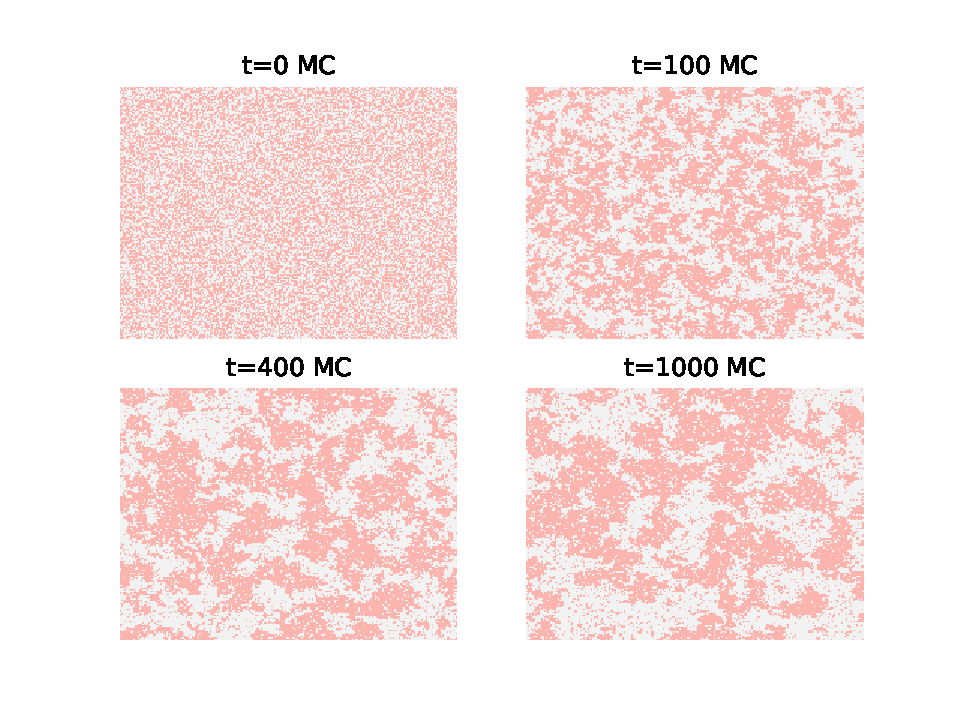
\includegraphics[width=0.9\linewidth]{intro/clusterization.pdf}
    \caption{Phénomène d'aggrégation à partir d'un refroidissement (\textit{quench}) dans un modèle d'Ising de $T=\infty$ à $T=T_C$ pour différents temps en étapes de Monte Carlo, pour un système $600 \times 600$ avec une dynamique non-conservée de Glauber.}
    \label{clusterization}
\end{figure}

À température non nulle, les fluctuations thermiques vont créer un système non-uniforme possédant des clusters possédant une longueur de corrélation $\xi$. L'énergie d'interaction de ces clusters est donné par l'Hamiltonien de Ginzburg-Landau\cite[§ 45]{l_landau_physique_1990}
\begin{align}
    H_0 &= \int d^dx \frac{\kappa}{2}(\nabla \phi)^2 + V(\phi) =  \int d^dx \frac{\sigma}{2}(\nabla \phi)^2 + \frac{\lambda}{2}(\phi^2-1)^2
    \label{hamil-mean-field}
\end{align}
où le premier terme correspond à la tension superficielle cherchant à diminuer les variations au sein du système, et le second terme est un potentiel en double puit $V(\phi) = \frac{\lambda}{2}(\phi^2-1)^2$ \ref{double-puits} simulant une interaction repoussante entre les deux types de particules. Ce terme explique la création de clusters de la figure \ref{clusterization}.

Dans les expériences en laboratoire, les systèmes sont souvent couplés à des champs magnétiques ou chimiques $h(x)$ d'Hamiltonien
\begin{align}
    H_1 &= - \int d^dx h(x)\phi(x)
    \label{champ-externe}
\end{align}
qui induit un changement de stabilité entre les phases, le signe négatif étant pour que le système s'aligne sur le champ. 
\begin{figure}
    \centering
    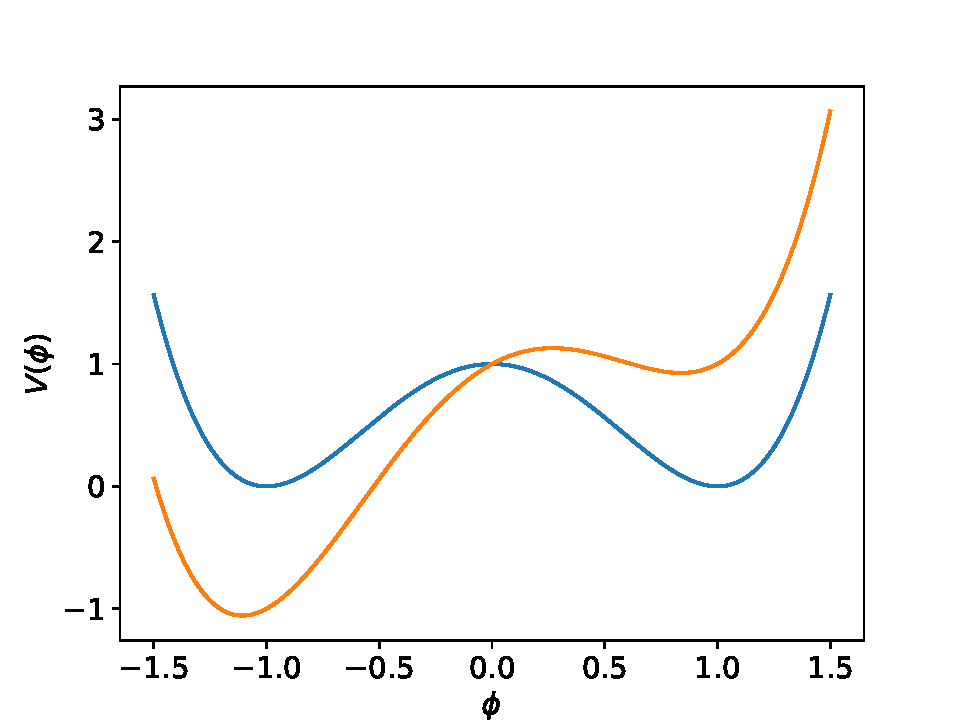
\includegraphics[width=0.5\linewidth]{intro/shift.pdf}
    \label{double-puits}
    \caption{Potentiel en double puits \ref{hamil-mean-field} pour $\lambda = 1$ en bleu. Le potentiel a deux positions d'équilibre stables à $\pm1$, ce qui induit une séparation de phase. En orange, l'ajout d'un champ externe \ref{champ-externe} constant $h \phi(x)$ rend la phase $+1$ métastable.}
\end{figure}

La fonction de partition du système s'écrit
\begin{align}
    \mZ = \int D[\phi] e^{-\beta( H)}
\end{align}
avec $H= H_0 + H_1$. Dans le cas où le paramètre d'ordre est conservé avec pour valeur fixe $M$, un terme supplémentaire égal à $\delta(\int d^dx \phi(x)-M)$ apparaît. Ce terme empêche toute résolution analytique de la fonction de partition, mais nous verrons plus tard certaines méthodes pour contourner ce problème.
La valeur moyenne de $\phi$ est alors
\begin{align}
    <\phi> = - \frac{\delta F}{\delta h(x)}
\end{align}
qui est nul en l'absence d'un champ extérieur $h(x)$. La fonction de corrélation à deux points de cet Hamiltonien est donné par 
\begin{align}
    C(x,y) = <\phi(x)\phi(y)> =  \frac{k_B T}{\sigma} \int_q \frac{e^{iq(x-y)}}{\xi^{-2}+ q^2}
\end{align}
et le facteur de structure  par
\begin{align}
    S(k) = < \tilde{\phi}(k)\tilde{\phi}(q)> = (2\pi)^d \delta_{k,q} \frac{k_B T}{\sigma} \frac{1}{\xi^{-2}+ q^2}
\end{align}
où l'on voit apparaître ici la longueur de corrélation à l'équilibre $\xi$. 

Dans l'ensemble grand-canonique, les particules ont la possibilité de se transformer en d'autres particules par réaction chimique ou par exemple inversion des spins dans un système ferromagnétique. L'équation dépendante du temps de Ginzburg-Landau (TDGL) décrit l'évolution du champ moyen en minimisant l'énergie libre du système
\begin{align}
    \frac{\partial \phi}{\partial t} &= - \alpha \frac{\delta H}{\delta \phi} \\
    &= \frac{\delta H}{\delta h} \frac{\delta h}{\delta \phi}
    \label{tdgl}
\end{align}
Le terme $\alpha$ est un coefficient cinétique décrivant le temps de relaxation du système. La minimisation de l'énergie tend à minimiser l'interface entre les différentes phases ainsi qu'à privilégier les phases homogènes. Dans un système infini, afin de minimiser la tension superficielle, les clusters grandissent au fur et à mesure de sorte que la longueur de corrélation $\xi$, qui décrit la longueur typique des phases, augmente comme $\xi(t) \propto t^{1/2}$.

Ces clusters sont définis pas l'interface\footnote{Dans les systèmes 1D, on retrouve le terme de mur entre deux domaines (\textit{domain wall}).} comme une courbe imaginaire où nous avons, en moyenne, un très fort gradient du champ $\phi$. 
En considérant que de part et d'autre du système nous avons deux phases différentes complètement homogènes selon l'axe des $z$, c'est-à-dire $\phi(z \to -\infty) = -1$ et $\phi(z \to +\infty) = +1$, on peut minimiser l'énergie libre selon $z$ afin d'obtenir le profil de l'interface. L'équation $\frac{\delta H}{\delta \phi} = 0$ nous donne une équation différentielle du second ordre en $\phi$ qui a pour solution selon l'axe $z$
\begin{align}
    \phi(z) = \tanh(\frac{1}{\xi_\perp} (z-h))
    \label{profil-phi}
\end{align}
où $\phi(z)$ est moyennée sur les autres variables spatiales et sur le temps, $\xi_\perp = (2\lambda)^{-\frac{1}{2}}$ est la largeur moyenne de l'interface, et $h$ est la hauteur moyenne de l'interface, que l'on peut fixer comme on le désire. Bien sûr, cette équation n'est valable qu'à la frontière entre deux domaines. Proche d'une transition de phase, la longueur de corrélation de l'interface $\xi_\perp$  diverge selon des exposants critiques spécifiques à chaque classe d'universalité. Pour une étude complète des exposants critiques pour chaque classe d'universalité, se référer à \cite{pelissetto_critical_2002}. 

{\color{red} réécrire}
La tension superficielle est donnée par l'énergie apportée par l'interface comparée à un milieu parfaitement homogène, c'est-à-dire où le terme $\frac{1}{2}(\nabla \phi)^2$ de l'hamiltonien est nul. La densité d'énergie par unité de surface est donc
\begin{align}
    \sigma = H_{inhomogène} - H_{homogène} = \int_{-\infty}^\infty dz \left(\frac{\partial \phi}{\partial z} \right)^2
\end{align}

Dans le \textbf{modèle B}, c'est-à-dire dans l'ensemble canonique, les particules ne peuvent réagir chimiquement entre elles. Avec l'agitation thermique, les particules auront cependant tendance à se déplacer, en échangeant leur position avec celle de leur plus proche voisin. Cette dynamique locale, qui décrit les phénomènes locaux comme la diffusion, est régie par l'équation de Cahn-Hillard\cite{cahn_free_nodate,langer_new_1975,kawasaki_growth_1978}
\begin{align}
    \frac{\partial \phi}{\partial t} = D \nabla^2 \frac{\delta H}{\delta \phi} 
    \label{cahn-hillard}
\end{align}
où $D$ est la diffusivité des particules. Dans cette dynamique plus lente, la taille typique des clusters est de l'ordre de $\xi(t) \propto t^{1/3}$.

\begin{figure}
    \centering
    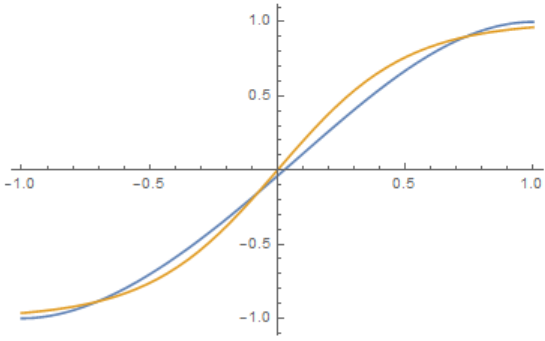
\includegraphics[width=0.5\linewidth]{intro/profil-KawVsGlau.png}
    \caption{Profil de l'interface pour un paramètre d'ordre conservé (orange) et non-conservé (bleu) avec les conditions aux limites $\phi(+\infty)-1$ et $\phi(+\infty)=+1$. Pour le modèle non-conservé, la résolution de l'équation \label{langevin-kawasaki} nécessite deux autres conditions supplémentaires. Nous avons donc mis $\phi(-1)=-1$,$\phi(1)=1$,$\phi'(-1)=\phi'(1)=0$. {\color{red} relancer code en résolvant la solution conservée au lieu de tanh(2x). Besoin mathematica.}}
\end{figure}

L'ajout d'un terme de bruit thermique aux équations de Langevin \ref{tdgl} et \ref{cahn-hillard} leur donne une la même allure que les modèles \textbf{A} et \textbf{B} respectivement de la théorie de la dynamique au point critique\cite{hohenberg_theory_1977}. Les équations précédents sont bien une approximation à $T=0$.


    \section{Taille finie et effet Casimir critique}
    
Sans perte de généralités en 3D, supposons un système de taille $L\times L' $ où $L<L'$. L'énergie libre $F(\beta,L,L') = - \frac{1}{\beta} \ln ( Z(\beta,L,L'))$ est une grandeur extensive lorsque la longueur de corrélation est plus petite que la taille du système $L$. 
Cette énergie libre peut se décomposer entre l'énergie de chaque phase $\omega_{bulk}$ et l'énergie de tension superficielle aux interfaces $\omega_{surf}$ \cite[§4]{cardozo_finite_2015}. À noter qu'à haute température dans un système complètement homogène, ce dernier terme disparaît.

Cependant, lorsque $\xi \simeq L$, la contrainte exercée sur les fluctuations thermiques par les conditions aux bords implique une modification de l'énergie libre, créant une force les parois. Cet effet, premièrement prédit Hendrik Casimir\cite{h_b_g_casimir_attraction_1948}, fut étendu aux systèmes critiques\cite{nikolic_is_2017}, où la divergence de la longueur de corrélation rend les expériences bien plus faciles\cite{nguyen_controlling_2013}.

L'énergie libre d'un tel système se décompose maintenant en 
\begin{align}
    \Omega(\beta,L,L') = L \omega_{bulk}(\beta) + \omega_{surf}(\beta) + L \omega_{ex}(\beta,L)
    \label{decomposition-energie}
\end{align}
où $\omega_{bulk}(L)$ est le surplus d'énergie libre due au confinement des fluctuations, qui devient nul dans la limite $L\to \infty$.

La force de confinement est définit par 
\begin{align}
    F_\perp(\beta,L) = - \frac{1}{L' }\frac{\partial \Omega}{\partial L} \bigg|_{\beta,L'} = -  \omega_{bulk}(\beta) -  \frac{\partial \omega_{ex}(\beta,L)}{\partial L}\bigg|_{\beta,L'}
\end{align}
où le premier terme est la pression exercée par le système, tandis que le second terme est la force de Casimir, qui n'est pas extensive. Afin d'extraire la force de Casimir, il suffit alors de soustraire deux quantités extensives, c'est-à-dire 
\begin{align}
    F_\perp(\beta,L_1) - F_\perp(\beta,L_2) =   \frac{\partial \omega_{ex}(\beta,L_2)}{\partial L_2}\bigg|_{\beta,L'} -  \frac{\partial \omega_{ex}(\beta,L_1)}{\partial L_1}\bigg|_{\beta,L'}
\end{align}
Puisque le surplus d'énergie est nul lorsque $L\to \infty$, on obtient que
\begin{align}
    F_\perp(\beta,L_1) - F_\perp(\beta,\infty) =   -  \frac{\partial \omega_{ex}(\beta,L_1)}{\partial L_1}\bigg|_{\beta,L'}
\end{align}
Cardozo et Holdsworth\cite[§5]{cardozo_finite_2015} ont développé une méthode numérique de calcul pour calculer numériquement cet excès. Nous y reviendrons plus tard.




    \section{Modèles d'interface}

Dans la réalité, les phases sont extrêmement inhomogènes, avec des bulles ou des digitations qui empêchent une description dynamique aisée de l'interface. Si l'on désire étudier l'interface de ces bulles ou digitations, où localement l'interface est bien définie par une fonction d'une seule variable, l'approche du champ moyen suffit. C'est le cas par exemple des régimes d'échelle (\textit{scaling regime}) où les interfaces se comportent toujours de façon correcte. De la même manière, ce régime d'échelle peut s'obtenir dans un milieu inhomogène en supposant qui'il est, au contraire, homogène. On suppose dans ce cas qu'il n'y a ni digitation ni bulles d'évaporation. Dans cette approximation l'interface est parfaitement définie en un point $h(x)$ (et non dans un profil comme dans \ref{profil-phi}. Tous les points du champ se trouvant en bas de l'interface prennent une unique valeur strictement différente de tous les points du champ au-dessus de l'interface. Sans perte de généralité, nous pouvons séparer les variables spatiales par $x$ pour toutes les coordonnées parallèles à l'interface et par $z$ la coordonnée transverse. Cela se traduit par
\begin{align}
    \phi(z) = f(z-h(x))
    \label{capillary-wave-theory}
\end{align}
où $f(x\greater 0) = \phi_1$ et $f(x\less 0) = \phi_2$. Notre système est maintenant complètement défini par l'interface $h(x)$ d'Hamiltonien
\begin{align}
    H = \int d^d x \frac{\sigma}{2} (\nabla h(x))^2 + V(h)
    \label{hamil-cwt}
\end{align}
où le premier terme est l'analogue au premier terme dans \ref{hamil-mean-field} représentant la tension superficielle et le potentiel $V$ fait référence au champ externe \ref{champ-externe}. 
Une interface se caractérise le plus généralement sa hauteur moyenne $<h(t)>$ de l'interface dans l'espace, et sa fonction de corrélation parallèle à l'interface qui décrit les modes de fluctuation de l'interface (sa rugosité)
\begin{align}
    C_\parallel(r,t) = <h(x,t)h(x+r,t)>_x - <h(0,t)>^2 = \sum_i A_i(\frac{r}{\xi_i}) 
\end{align}
Comme démontré dans la section \ref{sec_laser}, la décroissance spatiale est une somme de modes $i$ ayant des longueurs de corrélation différentes $\xi_i$ à décroissance exponentielle dont, dans la limite thermodynamique, seul le mode de plus basse énergie est observable. 
L'épaisseur de l'interface est donnée par $\omega(t) = \sqrt{C_\parallel(0,t)} = \sqrt{<h(t)^2> - <h(t)>^2}$. Cet observable est très facilement calculable dans les simulations de Monte Carlo.


    \subsection{Paramètre d'ordre non conservé}

Supposons une surface à laquelle viennent s'agréger des particules provenant d'un réservoir afin de créer un dépot. L'interface est alors définie par la hauteur de l'aggrégat par rapport à la surface de dépôt.

En partant de \ref{tdgl} et en insérant \ref{capillary-wave-theory} avec le changement de variable $u= z-h$, on a \cite{bray_interface_2001}
\begin{align}
    \frac{\partial h}{\partial t} f'(u) &= \nabla^2 h f'(u) - V'(f) + \xi(x,t)
\end{align}
avec $\xi(x,t)$ un bruit blanc gaussien. En multipliant les deux côtés par $f'(u)$ et en intégrant de $-\infty$ à $+\infty$, puisque le terme $ \int_{-\infty}^\infty V'(f) f'(u) du = 0$, on obtient l'équation d'Edwards-Wilkinson \cite{edwards_surface_1982} 
\begin{align}
     \frac{\partial h}{\partial t} = D + D \nabla^2 h +  \eta(x,t)
    \label{edwards-wilkinson}
\end{align}
où $\eta(x,t)$ est un bruit blanc de moyenne nulle et de corrélation 
\begin{align}
    <\eta(x,t)\eta(x',t')> = 2 D T\delta(x-x')\delta(t-t')
\end{align}
Ici $D+ \sqrt{2 D T} \eta(x,t)$ est le flux de particules s'aggrégeant en fonction du temps et $D \nabla^2 h$ dépend de la forme de l'interface, favorisant ou non le dépôt de particules à certains endroits.
La hauteur moyenne de l'interface varie donc comme $<h(t)> = Dt$. En se positionant dans le référentiel de l'interface via la transformation $h \rightarrow h + Dt$, on obtient
\begin{align}
     \frac{\partial h}{\partial t} =   \nabla^2 h +   \eta(x,t)
    \label{edwards-wilkinson-conesrved}
\end{align}
On remarquera la similarité entre cette équation et l'équation \ref{tdgl} en l'absence de potentiel en double puits et de champ externe.

L'ajoute d'un potentiel en double puits est cependant nécessaire afin d'obtenir une séparation de phases. L'équation KPZ\cite{kardar_dynamic_1986} étudie un champ moyen en $\phi^4$, ce qui introduit des nonlinéarités indispensables pour certaines propriétés des interfaces.
\begin{align}
     \frac{\partial h}{\partial t} = D \nabla^2 h +  \lambda (\nabla h)^2 + \eta(x,t)
    \label{kpz}
\end{align}

Il est intéressant de calculer la probabilité de distribution de la hauteur de l'interface par rapport à sa moyenne. La probabilité $p(h$) de trouver l'interface à la distande $h$ de la hauteur moyenne est donnée par l'équation de Focker-Planck\cite[p.241]{halpin-healy_kinetic_1995} associée à \ref{edwards-wilkinson-conesrved}
\begin{align}
    \frac{\partial p(h,t)}{\partial t} = - \int dx \frac{\delta}{\delta h} \left[ \left( D \nabla^2 h + \frac{\lambda}{2} (\nabla h) ^2 \right) p \right] + \int dx \frac{\delta^2 p}{\delta^2 h}
    \label{fokker-planck}
\end{align}
Dans le régime stationnaire $ \frac{\partial p(h,t)}{\partial t} = 0$ en une dimension, on trouve la distribution
\begin{align}
    p(h) = \frac{e^{-\frac{D}{2}\int_0^L dx (\nabla h)^2}}{Z}
    \label{stationary-distribution}
\end{align}
Cette distribution gaussienne ne prend pas en compte le terme nonlinéaire de l'équation KPZ, qui a donc, à l'équilibre en une dimension, le même profil que l'interface EW. Des études du profil KPZ dans le régime transient \cite{miettinen_experimental_2005,assis_dynamic_2015,g_foltin_width_1994,antal_dynamic_1996} donnent des résultats non symmétriques, puisque l'interface bouge avec le temps.

D'autres études de l'équation EW avec des conditions aux bords périodiques $h(0)=h(L)=0$ en 1+1 dimensions, prouve que l'hypothèse du régime d'échelle est justifié\cite{majumdar_airy_2005}, puisque la distribution de l'interface est de la forme 
\begin{align}
    p(h,L) = L^{-\frac{1}{2}} f(h L^{-\frac{1}{2}} )
\end{align}
avec la fonction $f(x)$ montré sur la figure \ref{fig-airy-majumdar}. L'exposant $\frac{1}{2}$ est l'exposant critique du modèle KPZ en une dimension.
\begin{figure}
    \centering
    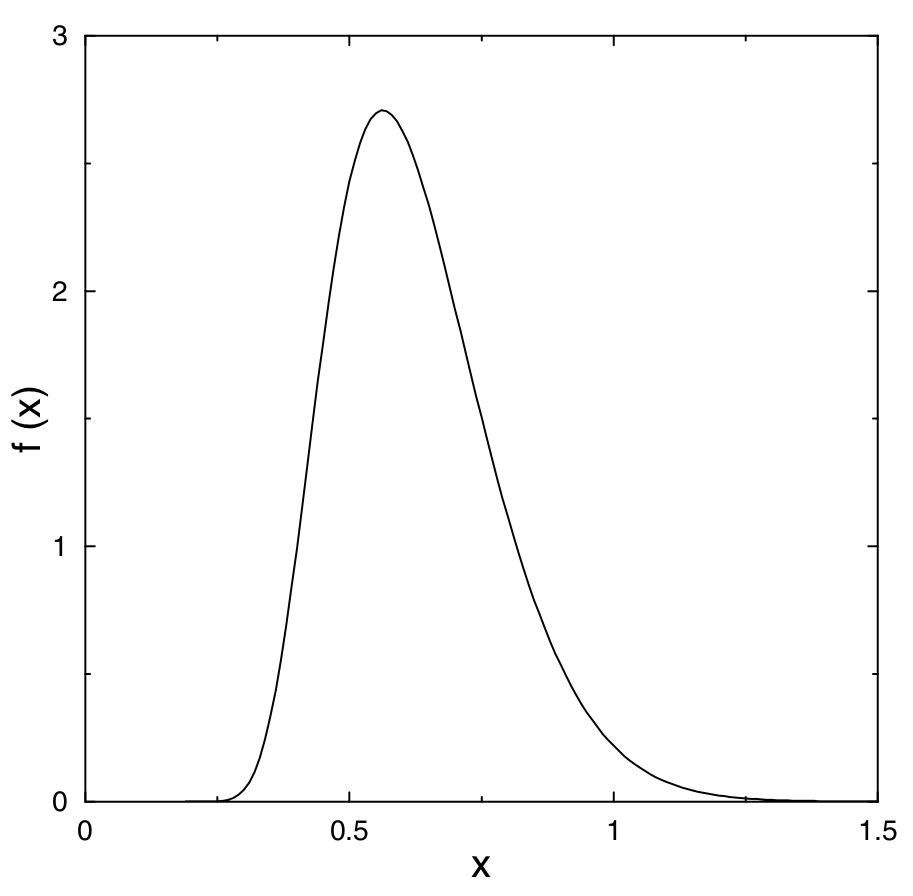
\includegraphics[width=0.5\linewidth]{intro/airyplot-majumdar.png}
    \caption{Fonction $f(x$) de la distribution des hauteurs d'une interface Edwards-Wilkinson avec des conditions aux bords périodiques\cite{majumdar_airy_2005} en 1+1 dimensions.}
     \label{fig-airy-majumdar}
\end{figure}


    \subsection{Paramètre d'ordre conservé}

Si l'on se place dans le référentiel du centre de l'interface, les équations \ref{edwards-wilkinson-conesrved} et \ref{kpz} conservent le paramètre d'ordre en moyenne. Néanmoins, la transformation $h \rightarrow h + Dt$ ne prend pas en compte les fluctuations thermiques qui viennent perturber l'interface, ce qui fait que $h(t) \neq cte$. L'astuce vient ici de \cite{kawasaki_diffusion_1966,kawasaki_correlation-function_1966}, où l'on reprend l'équation de Cahn-Hilliard-Cook pour les interfaces
\begin{align}
    \frac{\partial h}{\partial t} = D \nabla^2 \frac{\delta H}{\delta h} +  \eta(x,t)
\end{align}
qui nous donne l'équation Villain-Lai-Das Sarma\cite{villain_continuum_1991,lai_kinetic_1991}
\begin{align}
    \frac{\partial h}{\partial t} = - D \nabla^4 h + \lambda \nabla^2 (\nabla h) ^2 +  \eta(x,t)
\end{align}
qui a fait l'objet de nombreuses études\cite{kim_conserved_1994,assis_dynamic_2015}.

L'intérêt d'un tel système est qu'il est contraint à une dynamique locale qui permet d'obtenir un système hors-équilibre. La distribution de la hauteur de l'interface respecte ici aussi le régime d'échelle  \cite{oliveira_maximal-_2008,singha_renormalization_2016} dans le régime transient. 

    \section{Cisaillement d'une interface}
{\color{red} enrichir de résultats et manips}
Il suffit d'avoir une force conservative dans le système pour qu'il soit hors-équilibre, le cisaillement en est l'expression la plus simple. Le cisaillement intervient dans la sédimentation des particules, le mouvement forcé de particules chargées dans un champ électrique ou bien par la pression de radiation exercée par un laser. 
Dans un cisaillement, certaines particules ont tendance à bouger préférentiellement dans un sens par rapport aux autres particules, impliquant un flux non nul. Cette dynamique étant locale, elle ne peut exister que si le paramètre d'ordre est conservé. L'équation générale d'un système d'interface avec un cisaillement est\cite{bray_interface_2001-1,bray_interface_2001}
\begin{align}
     \frac{\partial h}{\partial t} + v \nabla h =  \mathcal{L} h +  \eta(x,t)
     \label{eq-cisaillement}
\end{align}
où l'opérateur $\mathcal{L}$ est associé au modèle A ou B, et le terme $v \nabla h$ est un terme de d'advection du au flux produit par le cisaillement. 


Le cisaillement le plus évident est un cisaillement homogène, par exemple un champ gravitationel qui sédimente les particules. Dans ce cas, le champ de vitesse $v$ étant constant, l'équation \ref{eq-cisaillement} est invariante par la transformation galiléenne $x \rightarrow x+vt$. 
Néanmoins de nombreuses expériences\cite{derks_suppression_2006} et simulations numériques \cite{leung_field_1986,rikvold_microstructure_2002,gonnella_nonequilibrium_2009,smith_driven_2010,smith_interfaces_2008,sadhu_non-local_2014,cohen_interface_2016} montrent que le cisaillement provoque un confinement de l'interface. Dans les expériences, cette invariance galiléenne est brisée par la disparité du champ de vitesse sur les différentes particules, comme expliqué en détail au chapitre \ref{chap-article-dean} \footnote{Ce chapitre a été publié dans \cite{dean_effect_2020}.}
Pour les simulations numériques, l'invariance est brisée par la dynamique même du système, puisque les mouvements sont fait séquentiellement. 

\chapter{Modèle Solid-On-Solid}
		  \section{Le modèle d'Ising}
  
  	Le modèle d'Ising fait partie de la catégorie des modèles sur réseau où l'interaction entre les particules du système se fait uniquement entre les plus proches voisins. Chaque particule au site $i$ possède deux états différents que l'on note $\sigma_i = \pm 1$, analogues aux spins en mécanique quantique. L'Hamiltonien d'un tel modèle s'écrit alors
\begin{equation}
	\mH =  - \sum_{\langle i j >} J_{ij} \sigma_i \sigma_j + \frac{V(\sigma_i)+V(\sigma_j)}{2}
\end{equation}
où $\langle ij >$ dénotent deux premiers voisins, $J_{ij}$ l'énergie d'interaction entre deux sites et $V(\sigma_i)$ le potentiel au site $i$.
En général, le modèle d'Ising est utilisé avec une énergie d'interaction constante entre tous les spins, soit $J_{ij} = J$. Les systèmes les plus connus possédant une énergie d'interaction non-constante sont  \textbf{trouver quelques exemples}.

En faisant la transformation\cite{ref23David} $n_i =  \frac{\sigma_i +1}{2}$ afin que $n_i(\sigma_i = 1) = 1$ et $n_i(\sigma_i = -1) = 0$, on obtient l'hamiltonient
\begin{equation}
	\mH =  - \sum_{\langle i j >}  J_{ij} \left( 4 n_i n_j -2 ( n_i+n_j) + 1 \right)+ \sum_{\langle i j >}  J_{ij} \frac{V(\sigma_i)+V(\sigma_j)}{2}  
\end{equation}
où le terme constant $\sum_{\langle i j >}  J_{ij}$ ne modifie la fonction de partition $\mZ$ que d'une constante peu importante pour les propriétés à l'équilibre du système. On définit alors 
\begin{equation}
	\mH_{LG} =  - 4 \sum_{\langle i j >}  J_{ij}  n_i n_j  + 2 \sum_{\langle i j >}  J_{ij}  (n_i+n_j) + \sum_{\langle i j >}  J_{ij} \frac{V(\sigma_i)+V(\sigma_j)}{2}  
\end{equation}
Le deuxième terme s'identifie à la présence d'un potentiel chimique pour les particules liquide-gaz. Une phase magnétique positive dans le modèle d'Ising s'apparente dès lors à un état de haute densité (un liquide), tandis qu'une phase négative est considérée comme une phase de basse densité, c'est-à-dire un gaz.
Ce modèle représente également un mélange binaire\cite{} entre deux types de particules $A$ et $B$ comme par exemple un polymère dans un solvant, les particules identiques s'attirant tandis que les particules d'un type différent se repoussent. 

En général, dans tous les modèles d'Ising étudiés, $J_{ij}$ est constante et égale à $J$. Nous prendrons cette approximation à partir de maintenant.

En absence de potentiel, le système est statistiquement découpé en amas (\textit{bulk}) de spins du même signe\ref{amas-quench}. La longueur de corrélation   $\mC= \mC(T,J)$ dépend fortement de la température et diverge près de la température critique. Une étude détaillée des grandeurs du modèle d'Ising proche du point critique\cite{onsager,3d} peut être retrouvée dans \cite{these_david}.

L'étude de l'interface entre les phases $+$ et $-$ nécessite la brisure de la symétrie de translation au sein du système. Cela peut se faire facilement soit par des conditions aux bords non-périodiques dans une direction, soit  par la présence d'un champ magnétique non-uniforme du style $V(y) = h |\frac{L_Y}{2}-y|$. 
Dans le cas de conditions aux bords fixes avec par exemple les spins de la rangée $0$ étant positifs et ceux de la rangée $L_Y$ négatifs, des clusters vont se former et créer une interface au milieu. Il est possible de favoriser une phase par rapport à l'autre grâce à un potentiel chimique (ou champ magnétique) $V(h_i) = -h \sigma_i$ \cite{}. Ce genre de modèle s'assimile à un système d'absorption d'un gaz sur réseau\cite{} ou de la croissance d'un matériau sur un substrat\cite{}

Le choix d'un champ magnétique du style $V(y) = - B |\frac{L_Y}{2}-y|$ modélise quant à lui l'effet d'un champ  sur un liquide binaire selon les expériences de Delville\cite{}. La présence d'un laser dans certaines régions du système peut modifier localement le potentiel chimique des particules, favorisant la présence d'un type par rapport à l'autre. L'épinglage\cite{} (\textit{pinning}) de l'interface auprès de la ligne de démarcation permet de l'étudier loin des bords du système.		
		
		\section{Hamiltonien}
	
Quelle que soit la méthode utilisée, le système se simplifie dès lors que nous désirons étudier uniquement l'interface d'un système et non son ensemble, telles que les longueurs de corrélations dans le \textit{bulk}, l'aimantation moyenne, la chaleur spécifique ou la susceptilibté magnétique. À très basse température, les interfaces sont bien délimitées et il y a très peu de gouttes d'évaporations d'une phase dans l'autre. En considérant le système très peu mélangé, il est possible de définir la présence d'une phase par rapport à la hauteur $h_i$ de l'interface. Chaque spin prend la valeur
\begin{align*}
	\sigma_{i,j} = \sgn(h_i-j)
\end{align*}
où la fonction $\sgn(x)$ est égale à $+1$ si $x>=0$ et à $-1$ sinon. Cela revient à considérer que l'énergie d'interaction perpendiculaire est prohibitif par rapport aux liaisons parallèles à l'interface $J_\perp \gg J_\parallel$. 

\begin{figure}
	\centering
	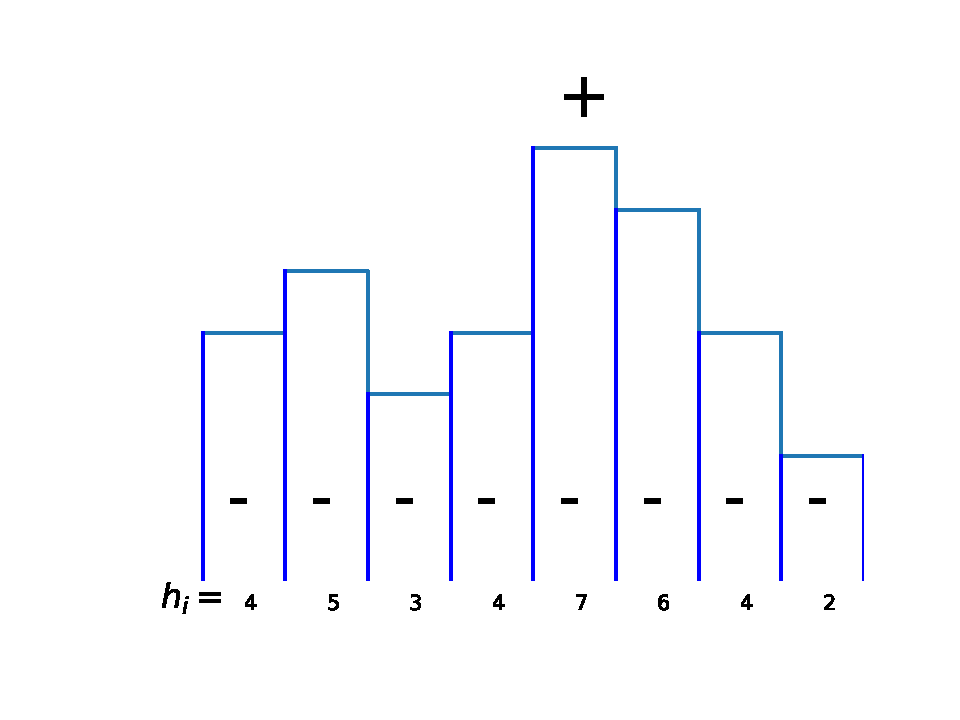
\includegraphics[scale=1]{isingtosos/sos-indiscernable.pdf}
	\caption{Une configuration possible de modèle SOS. Dans la i-ème colonne le bord horizontal de l'interface passe à la hauteur $h_i$. Toutes les particules au-dessus de l'interface sont des spins positifs et négatifs en dessous. La représentation classique du modèle SOS diffère de ce schéma par l'hypothèse que les particules sont discernables. Nous y reviendrons plus tard.}
\end{figure}


En utilisant l'identité $\min(a,b)-\max(a,b)=|a-b|$, on a
\begin{align*}
    \sum_{j=0}^L \sgn(h-j)\sgn(h'-j) = L - 2 |h-h'|
\end{align*}
Ainsi, pour un système de longueur $L_X$ et de largeur $L_Y$ l'hamiltonien du modèle d'Ising en absence de potentiel se réécrit comme 
\begin{align}
    H = 4 J L_X (2-L_Y) +4J \sum_i |h_i-h_{i+1}|
\end{align}
Le terme $|h_i-h_{i+1}|$ représente la surface de contact horizontale entre les deux phases qui dépend directement de la hauteur, tandis que le terme constant représente la surface de contact verticale.
En retirant la partie constante de l'énergie et simplifiant $4 J = J$ et en gardant $L_X = L$, nous obtenons l'hamiltonien du \textbf{modèle Solid-On-Solid}
\begin{align}
    H = J \sum_i |h_i-h_{i+1}|
    \label{hamil-sos}
\end{align}

Nous avons ici réussi à réduire la dimensionalité du système en ne prenant en compte que la hauteur $h_i$ au site $i$. L'énergie du système est alors décrite par la différence de hauteur entre deux sites voisins, et $\beta J$ prend ici alors le rôle de la tension de surface.

Puisqu'il n'y a plus de transition de phase possible dans ce modèle, la température critique $\beta_C$ du modèle d'Ising n'a plus de rôle à jouer ici. Pour rester dans le domaine de l'approximation, si nous désirons comparer les résultats avec ceux du modèle d'Ising, il faudra veiller à rester dans le domaine $T \less T_C$, l'approximation étant de plus en plus valable plus la température est basse. Par la suite, puisque nous désironts étudier le modèle SOS et non le comparer avec le modèle d'Ising, nous prendrons, sauf cas contraire explicité, $\beta = \beta_C \simeq 0.44$ et $J=1$ par soucis de simplicité. 

  \section{Matrice de Transfert}

	De manière plus générale, l'Hamiltonien d'un système avec des interactions entre les particules peut se réécrire comme $H = \sum_{\langle ij >} H(i,j)$ avec
\begin{align*}
  H(h_i,h_{i+1}) = f(h_i,h_{i+1}) + V(h_i,h_{i+1}) 
\end{align*}
où $f(h_i,h_j)$ est l'énergie d'interaction entre plus proches voisins et $V(h_i,h_j)=\frac{V(h_i)+V(h_j)}{2}$ le potentiel symmétrisé.
La fonction de partition de notre système s'écrit alors 

\begin{align*}
 Z = \sum_{h_1 h_2 ... h_L} e^{- \beta \sum_{i} H(h_i,h_{i+1})}  
   = \sum_{h_1 h_2 ... h_L} \prod_{i} e^{-\beta H(h_i,h_{i+1})} 
\end{align*}
La matrice $T(i,j) = e{-\beta H(i,j)}$ est appelée matrice de transfert. Cette matrice est périodique aux bords, c'est-à-dire $T(L,L+1) = T(L,1)$ et est symétrique, ce qui implique qu'elle est diagonalisable dans la base des vecteurs propres $|\lambda >$ de valeur propre $\lambda$. On dénote par $\lambda_0$ la plus grande valeur propre de $T$, -par $\lambda_1$ la deuxième plus grande valeur propre et ainsi de suite.
Ainsi la fonction de partition devient\cite{}
\begin{align}
  Z = \sum_{\sigma_1 \sigma_2 ... \sigma_{L}} \prod_{i} T(i,i+i) = Tr T^L  = \sum_\lambda \langle\lambda | T^L | \lambda> = \sum_\lambda \lambda^L
\end{align}

Dans la limite thermodynamique $L \to \infty$, seuls les plus grands vecteurs propres jouent un rôle. Afin de calculer les observables de notre système, il convient d'introduire la matrice des hauteurs $\tilde{M}(i,j) = \delta_{ij} i$. Nous avons donc \footnote{Pour une démonstration plus détaillée sur les matrices de transfert, se référer à \cite{matrice_transfert}}
\begin{itemize}
	\item L'énergie libre par site :  
	\begin{align}
		F =  - \frac{1}{L \beta} \ln(Z) \simeq - \frac{1}{L \beta } \ln( \lambda_0)
	\end{align}
	\item La densité de probabilité qu'un site se trouve à la hauteur $h$ : 
	\begin{align}
		p(h) = \frac{1}{Z} \sum_\lambda \lambda^L \langle\lambda | h >^2 \simeq \langle \lambda_0 | h >^2
	\end{align}
	\item La magnétisation moyenne :
	\begin{align}
		M = \langle h > = \langle \lambda_0 | \tilde{M} | \lambda_0 > 
	\end{align}
	\item La variance des hauteurs :
	\begin{align}
		\sigma = \langle (h - \langle h >)^2 > =  \langle \lambda_0 | \tilde{M}^2 | \lambda_0 >
	\end{align}
\end{itemize}

	\section{Stabilité de l'interface}

	Soit $\psi_\lambda(h)$ la projection du vecteur propre associé à la valeur propre $\lambda$ de la matrice de transfert sur la base des hauteurs dans un système infini de par et d'autre de l'interface. En absence de potentiel\cite{guyer1979}, l'équation du vecteur propre donne
\begin{align}
	\sum_{h=-\infty}^\infty T(h,h') \psi_\lambda(h) = \lambda \psi_\lambda(h')
\end{align}
En introduisant l'ersatz $\psi_\lambda(h) = \alpha^h$ qui respecte la symétrie du système, et en séparant de la somme les termes pour $h$ négatifs et positifs, on trouve aisément que 
\begin{align}
	\frac{\sinh(\beta J)}{\cosh(\beta J)-(\alpha+\frac{1}{\alpha})} \alpha^{h'} = \alpha^{h'} \lambda
\end{align}
Dans la limite thermodynamique, la probabilité de présence de l'interface à la hauteur $h$ est $p(h) = <\lambda_0|h>^2 = |\psi_0(h)|^2$. Le système ne possédant aucune brisure de symétrie particulière, la probabilité $p(h)$ se doit d'être bornée pour tout $h$. Dès lors, l'ersatz supposé $\psi_\lambda(h) = \alpha^h$ implique que $\alpha$ soit de la forme $e^{ik}$ où $k$ est la longueur d'onde associée à la valeur propre $\lambda$. On obtient que 
\begin{align}
	\psi_k(h) =& e^{ikh} \\
	\lambda_k =& \frac{\sinh(\beta J)}{\cosh(\beta J) - \cos(k)}
\end{align}


Dans le cas plus général où l'hamiltonien s'écrit de la forme $T(h,h') = f(|h-h'|)$, on trouve 
\begin{align}
	\lambda_k = \sum_{h=0}^\infty f(h)(\alpha^h+\alpha^{-h}) - f(0)
\end{align}

L'existence d'une solution de ce genre indique que l'interface n'est pas localisée dans le cas d'un système infini (ou semi-infini) en absence de tout potentiel, ce qui conduit à de nombreux problèmes numériques. 

Il est à noter qu'à $\beta=0$, c'est-à-dire pour une température infinie, la matrice de transfert est uniformément égale à $1$, menant à des vecteurs propres nuls. Dans cette limite, l'interface n'existe plus, le modèle SOS n'est donc pas valable. De même, pour une température nulle $\beta=\infty$, la matrice de transfert devient la matrice identité. Les valeurs propres deviennent toutes égales à $1$ et les vecteurs propres sont $\psi_i(h) = \delta_{h,i}$ où ici $i$ est l'indice de la i-ème valeur propre $\lambda_i = 1$. La probabilité de trouver l'interface à la hauteur $h$ devient $p(h) = \frac{1}{Z}\sum_{i} <\lambda_i | h >^2 = 1$. La température nulle a pour effet de geler l'interface sur une seule hauteur, mais toutes les hauteurs sont équiprobables. Bien que les micro-états soient extrêmement différents que pour une température finie, les propriétés macroscopiques sont identiques à cause du même poids statistique associé à chaque état.


Historiquement, une manière facile de localiser l'interface est de rajouter un potentiel $V(h) = -B \delta_{h,0}$ \cite{chui}. La présence du potentiel n'affecte pas la parité du système mais peut introduire un surplus de particules en $0$. La recherche d'un état lié nous donne un ersatz de la forme 
\begin{align}
	\psi_\lambda(h) = \begin{cases} |\alpha|^h & \text{si } h \neq 0 \\ \psi_{\lambda,0} & \text{sinon} \end{cases} 
\end{align}
L'équation du vecteur propre devient
\begin{align}
	\sum_{h=-\infty}^\infty e^{\beta |h-h'|- \beta B \delta_{h,0}} \psi_\lambda(h) = \lambda \psi_\lambda(h')
\end{align}
En notant $T(h,h') = R^{|h-h'|}$ pour $h \neq h' \neq 0$,  on obtient la même équation à un signe près dans l'exposant que l'on soit à $h'>0$ ou $h'>0$
\begin{align}
	\left( \frac{R}{\alpha} \right)^{\pm h'} \left[ \psi_{\lambda,0} + \frac{R \alpha}{1 - R \alpha} + \frac{\alpha}{R - \alpha} \right] + \left[ \frac{1}{1-R \alpha} - \frac{R}{R-\alpha} \right] = \lambda
\end{align}
Puisque cette équation est vraie pour tout $h'$, le premier terme doit être nul, ce qui nous donne
\begin{align}
	\psi_{\lambda,0} &= - \frac{\alpha}{R-\alpha}-\frac{R \alpha}{1-R \alpha} \\
	\lambda &= \frac{1}{1-R \alpha} - \frac{R}{R-\alpha}
\end{align}
L'équation du vecteur propre à $h'=0$ nous donne par ailleurs 
\begin{align}
	\psi_{\lambda,0} + 2 \frac{R \alpha}{1-R \alpha} = \lambda \psi_{\lambda,0} e^{-\beta B}
\end{align}
L'existence d'une solution cohérente $\alpha < 1$ autorise la présence d'une interface localisée grâce au pinning.

D'autres méthodes existent pour confiner l'interface. Le cisaillement d'une interface diminue sa largeur et permet de la localiser dans l'espace. On peut également proposer deux potentiels chimiques différents pour chaque phase à une hauteur de l'interface prédéfinie, comme le ferait un laser dans les expériences de cisaillement\cite{delville} dans un système semi-infini. Cet cas sera étudié plus loin. Dans un système infini, une autre possibilité est de définir un champ magnétique symétrique rendant plus difficile la présence de l'interface loin de $0$. Nous utiliserons ici un potentiel du style
\begin{align}
		  V(h) = B |h|
\end{align}

Il est facile de se convaincre que loin de $0$ le coût énergétique est si grand que la probabilité que l'interface s'y trouve soit petite, impliquant que l'interface est localisée. La position moyenne de l'interface se situe au minimum du potentiel qui est dans ce cas $0$. 


	\section{Ensemble canonique}



\begin{figure}[h]
	\centering
	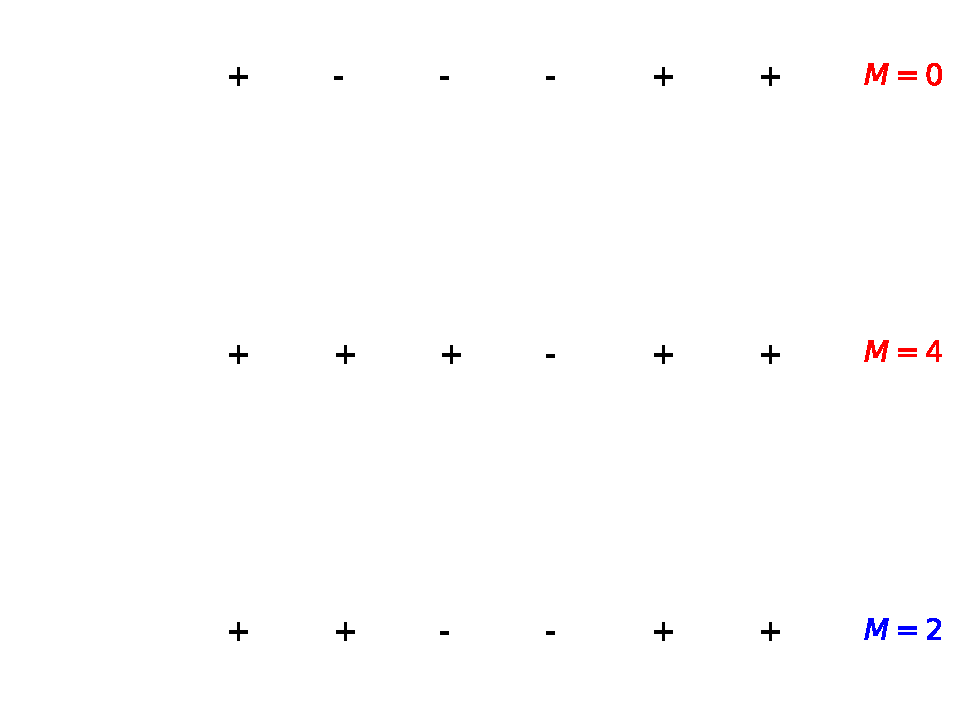
\includegraphics[scale=1]{isingtosos/figure-canonique.pdf}
	\caption{Dans un modèle d'Ising à 1D, afin d'avoir une magnétisation moyenne du système à $<M>=2$, tous les états sont acceptés tant qu'il y en a d'autres afin de respecter la moyenne. Dans l'ensemble canonique, on n'a plus $<M>=2$ mais $M=2$, interdisant les micro-états rouges.}
\end{figure}

Dans l'ensemble grand-canonique, le nombre de particules dans le système varie, dépendant du potentiel chimique vis-à-vis du réservoir dans lequel il est inséré, ce qui permet à l'interface de bouger librement. Lorsque l'on se place dans un système canonique, le nombre de particules (c'est-à-dire la magnétisation totale $M$) est fixe, ce qui introduit une contrainte dans la fonction de partition
\begin{align}
	 Z(M) = \sum_{h_1 h_2 ... h_L} e^{- \beta \sum_{i} H(h_i,h_{i+1})}  \delta(\sum_i h_i = M)
\end{align}
avec la relation vis-à-vis de l'ensemble grand-canonique en l'absence de potentiel chimique
\begin{align}
	 \Xi = \sum_{M} Z(M) 
\end{align}
La position moyenne de l'interface est maintenant définie et beaucoup d'états sont interdits, ce qui change énormément les propriétés thermodynamiques de la matrice de transfert comme la distribution des hauteurs de l'interface, même si la moyenne reste la même. Malheureusement, il est impossible de réécrire la contrainte dans le langage des matrices de transfert, empêchant ainsi de calculer analytiquement les différences entre les deux ensembles. Il est possible de construire la fonction de partition \textit{ab initio}, mais le grand nombre de sites et de hauteurs permises dans un système classique empêchent le calcul dans un temps raisonnable. 


	\section{Indiscernabilité des particules : Particle-Over-Particle}
	
Dans le modèle d'Ising, les particules sont discernables puisque labellisées par leur position $(i,j)$. Cette discernabilité pose problème lorsque l'on utilise le modèle pour un système de gaz sur réseaux ou de fluides binaires par exemple. À cet égard le modèle SOS est meilleur, puisque la discernabilité ne concerne plus que les sites $i$ contenant $h_i$ particules indiscernables. 
En prenant le point de vue atomiste présent dans le modèle d'Ising, nous pouvons suivre la position de chaque particule au sein de nos sites. Cela a plusieurs implications.
La première, c'est qu'en général, seules les couches proche de l'interface sont actives, tandis que les mouvements dans le \textit{bulk} sont bien plus lents. Ainsi, en prenant une particule au hasard dans nos simulations numériques, il est possible de donner une mobilité différente aux couches du modèle SOS. Nous n'explorons pas ces systèmes dans la présente thèse. 
Deuxièmement, lors des algorithmes de Monte Carlo définit au chapitre suivant, la probabilité de choisir un site au hasard n'est pas la même que celle de choisir une particule au hasard ! 
La fonction de partition d'un système où les particules sont discernables s'écrit maintenant
\begin{align}
	Z = \sum_{h_1 h_2 ... h_L} e^{- \beta \sum_{i} H(i,i+1)} \frac{N!}{\prod_i n_i!} = N! \sum_{h_1 h_2 ... h_L} e^{- \beta \sum_{i} H(i,i+1) -\sum_i \ln(n_i!)}
\end{align}

Ce nouveau système, que l'on appellera - par analogie avec Solid-On-Solid - le modèle Particle-Over-Particle sera étudié de manière détailĺée dans les derniers chapitres.

\begin{figure}[h]
	\centering
	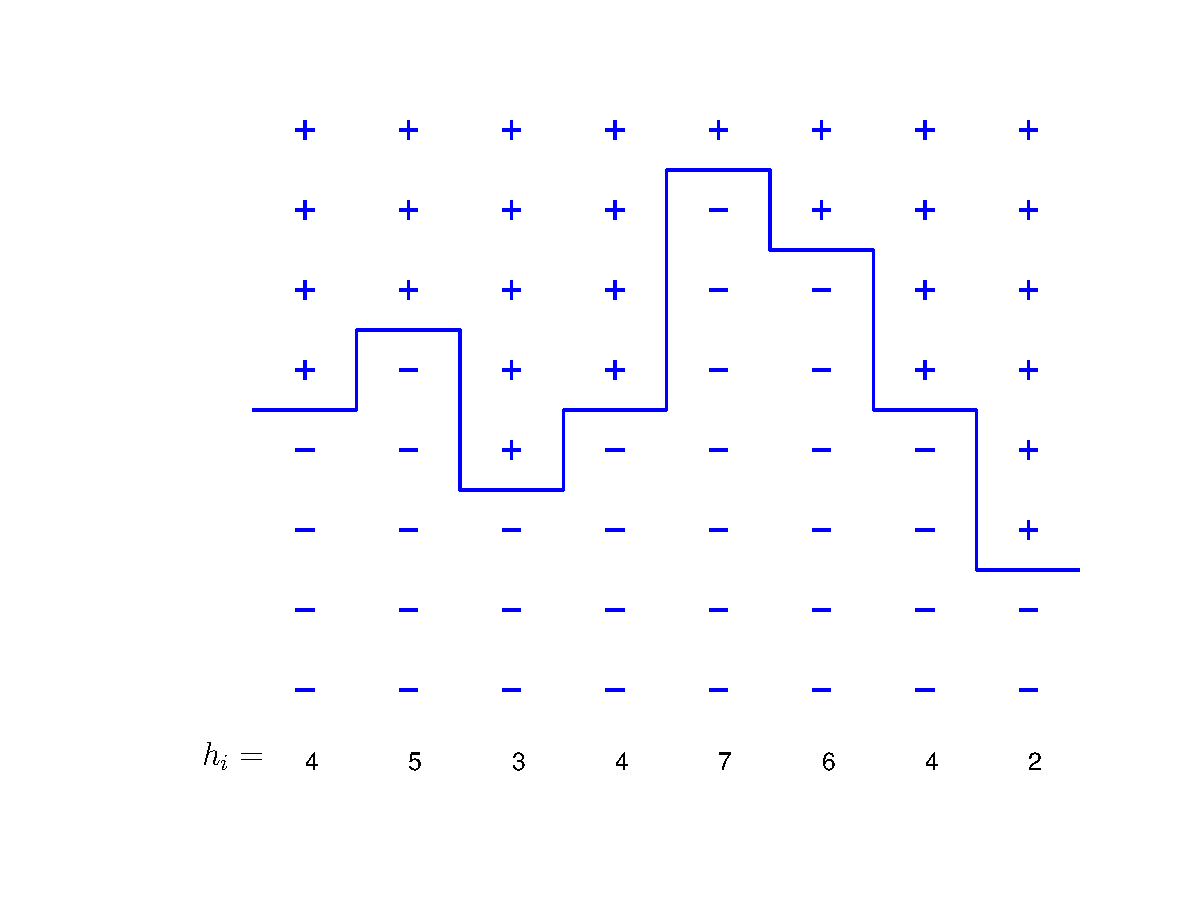
\includegraphics[width=0.7\linewidth]{isingtosos/figure-sos.pdf}
	\caption{Une configuration possible de modèle SOS lorsque les particules sont discernables. Cette représentation est la représentation classique dans la littérature.}
\end{figure}



\begin{comment}
		\section{SOS Hamiltonian}
		%%%%%%%%%%%%
		
		In the following, we present three Solid-On-Solid models with different magnetic fields. 
		The SOS interaction between nearest neighboors is of the form $f(i,j) = |h_i - h_j|$. 
		This kind of interaction prevents big fluctuations between two nearest neighboors and is directly related to the Ising model in the approximation where there are no overhangs between the two phases. \textcolor{blue}{see my notes for the derivation}
		
		In the absence of a magnetic field, the interface will fluctuate around its center. Shown below an typical SOS interface for an $L_X=50$ and a $L_Y=60$ after $10^5$ Monte Carlo steps.
		
		%\includegrapsics[width=10cm]{nomag.png}
		
		
		%%%%%%
		\subsection{Model $g(i) = h_i$ (model A)}
		%%%%%%
		
		This model replicates the effect of a homogeneous magnetic field. The bigger the magnetic field $B$ (which can be positive or negative), the further the interface is driven with a symetry breaking. 
		
		\begin{align}
		  H(i,j) = J |h_i-h_j| + B \frac{h_i + h_j}{2}
		\end{align}
		
		%\includegrapsics[width=10cm]{normal.png}
		
		For an infinite magnetic field, we clearly see that the interface gets flattened over on of the edge. The resulting single state avalaible in this limit is the flat interface, with all sites beeing over or under it, depending on the sign of $B$.
		
		In the limit $B \rightarrow \infty$, the interface will flatten to the bottom edge, resulting in a single state of energy 
		\begin{align}
		  F(B \rightarrow \infty) = - B L_Y
		\end{align}
		
		The free energy for at $B=0$ is thus given by align \ref{free_energy} as
		\begin{align}
		  F(0) = B L_X L_Y - \int_0^\infty m(B)dB
		  \label{energymodela}
		\end{align}
		with $m(B) = \langle\sum_i h_i> = L_Y$
		
		%%%%%%
		\subsection{Model $g(i) = |h_i|$ (model B)}
		%%%%%%
		
		This model uses a stagged magnetic field analoguous to the action of a laser on a binary mixture. The further we get from the mean position, the higher is the energy. In order to minimize the energy, the system will have a tendency to be pinned, leading to a very flat interface. 
		
		\begin{align}
		  H(i,j) = J |h_i-h_j| - B \frac{|h_i| + |h_j|}{2}
		\end{align}
		
		%\includegrapsics[width=10cm]{stagged.png}
		
		In the limit $B \rightarrow \infty$, the free energy $F$ will be equal to $0$, while the magnetisation $m(B \rightarrow \infty) = \langle\sum_i |h_i|> = 0$ also.
		
		%%%%%%
		\subsection{Model $g(i) = -|h_i|$ (model C)}
		%%%%%%
		
		This model is the same as the previous one, except with a switch of sign. In this case, the magnetic field will have a depinning effect leading to a scattering of the heights around both edges. \textcolor{red}{I don't really get yet the argument about the competition between entropy and energy.}
		
		\begin{align}
		  H(i,j) = J |h_i-h_j| - B \frac{|h_i| + |h_j|}{2}
		\end{align}
		
		%\includegrapsics[width=10cm]{negstagged.png}
		
		In the $B \rightarrow \infty$ limit, we have then a scattered system. How can we compute its free energy ? Sites will be at $h_i=\pm L_Y$ , leading to an easy $2\times 2$ transfer matrix.
		\begin{align}
		  Z = e^{\beta B L_Y L_X} Tr( (e^{-\beta J \frac{L_Y}{2} \sum_i |\sigma_i - \sigma_j| })^{L_X} )
		\end{align}
		where $\sigma_i = \pm 1$
		
		The transfer matrix is then given as
		
		\begin{align}
		T= e^{\beta B L_Y}
		  \begin{pmatrix}
		    1 & e^{-\beta 2 J L_Y} \\
		    e^{-\beta 2 J L_Y} & 1
		  \end{pmatrix}
		\end{align}
		Its eigenvalues are $\lambda_\pm = e^{\beta B L_Y}( 1 \pm e^{-\beta 2 J L_Y})$, giving a partion function 
		\begin{align}
		  Z = e^{\beta B L_Y L_X} \times ((1 - e^{-\beta 2 J L_Y})^{L_X} + (1 + e^{-\beta 2 J L_Y})^{L_X} )
		\end{align}
		
		The free energy from \ref{deffree_energy} is 
		\begin{align}
		  F(B\rightarrow \infty) = - L_Y B - \frac{1}{\beta} \ln \left( 1 + e^{-\beta 2 J L_Y} \right)
		  \label{energymodelc}
		\end{align}
		which, in the limit of $L_X \rightarrow \infty$ converges to \ref{energymodela}. This is easily explained as the energy to switch from a side to another increases so much that at some point the interface will be pinned to one of the edges, resulting in the same single state.
		
		\begin{figure}
		%  \includegrapsics[width=13cm]{comparison.pdf}
		  \caption{Computation of both terms in \ref{free_energy} in the limit $L_X \rightarrow \infty$ and $L_Y=30$ for the three different models. We see that models A and C have a very similar behaviour even for very small $B$. The linear fit does indeed give a relation $F(0) - F(B) = L_Y \times B$}
		\end{figure}
		
		%%%%%%%%%%%%
		\newpage
		\section{Numerical results}
		%%%%%%%%%%%%
		
		The diffusion of particles in a system can be mapped in an Ising model pretty easily if we assume the conservation of particles through time in our Monte Carlo dynamics. That means that $\sum h_i = K$, with $K$ a constant defined by the initial conditions. This condition can be enforced in the partition function if we only take the microstates satisfying our constraint. Sadly, this constraint is about the microstates and can not be transposed into our Hamiltonian, making the Transfer Matrix useless for such a case. 
		
		The question we want to adress is thus : how big is the difference between the constrained and the unconstrained dynamic in the computation of the free energy ? Is the limit $B^{\ast} \rightarrow \infty$ the same for the three models for both dynamics ? 
		Figure \ref{compGlau} conforts us in the conformity between the Glauber dynamic and the Transfer Matrix method. 
		
		\begin{figure}[h]
		%  \includegrapsics[width=13cm]{ModGlau.pdf}
		  \caption{Computation of the free energy (above) and the magnetisation (below) for the three models in a Glauber dynamics (unconstrained dynamics) through simulations (with error bars) and exact transfer matrix diagonalization.}
		  \label{compGlau}
		\end{figure}
		
		When comparing to the Kawasaki dynamic in Figure \ref{compKaw}, we start seeing some differences. First, in model A the magnetization of our system is always  equal to $0$, by construction of our Kawasaki dynamics, meaning that the computation of the free energy is a tricky one. Luckily, Model A is very similar to Model C with respect to the posible microstates, except some walls that do not add a significan free energy into the system. This means that the results we obtain in Model C are roughly the same as in Model A ! This allows us to drop Model A from the discussion from now on and get retrieve its general behaviour and properties from Model C.
		
		As expected, the constrained dynamics adds some variance with respect to the Transfer Matrix. 
		
		\begin{figure}
		%  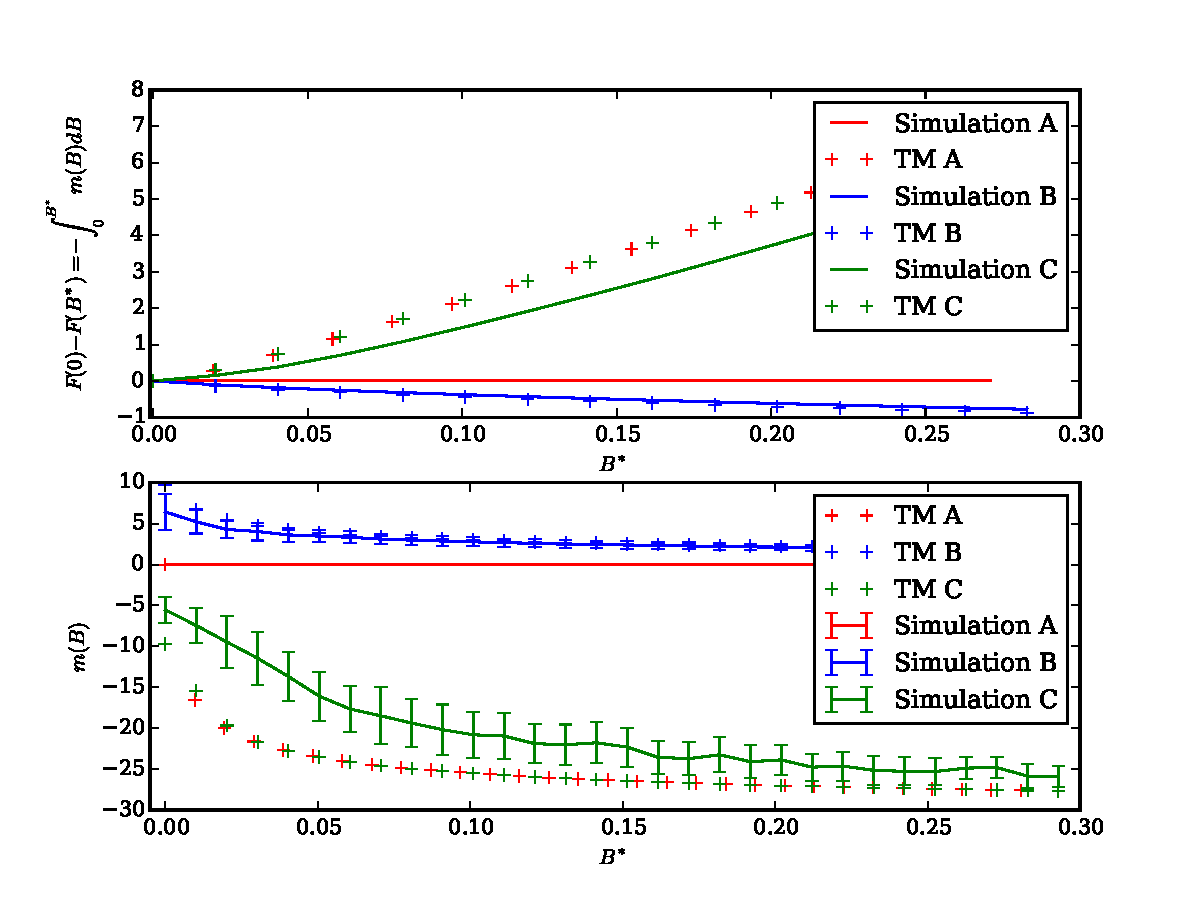
\includegraphics[width=13cm]{ModKaw.pdf}
		  \caption{Computation of the free energy (above) and the magnetisation (below) for the three models in a Kawasaki dynamics (constrained dynamics) through simulations (with error bars) and exact transfer matrix diagonalization. The error in magnetization of Model A is exactly equal to 0, by construction.}
		  \label{compKaw}  
		\end{figure}

  \section{Discretization of the system with respect to continuous models}
    \subsection{Correlation length and temperature}
\end{comment}
\chapter{Numerical methods}
\label{chap-sim}

In 1949, Metropolis \cite{metropolis_monte_1949} discovers a method to compute, through Monte Carlo simulations, the expectation value of statistical quantities. If $Q$ is an observable quantity of a statistical system, such as the total energy or density of particles per site, then the expectation value is computed by weighting its value over all configurations $C$ with respect to their statistical weight. If we consider the system to be at thermodynamic equilibrium, then every configuration $C$ follows the Gibbs-Boltzmann distribution, and the mean value $<Q>$ is
\begin{align}
    <Q> = \frac{\sum_{C} Q(C) \exp(-\beta E(C))}{\sum_{C} \exp(-\beta E(C))}
\end{align}
For example, in a SOS system of size $100\times100$ - which is small compared to the thermodynamic limit as discussed in figure \ref{fig-thermo-libre} - there exist $100^{100}$ different possible configurations. In comparison, numerical simulations can explore up to $10^9$ configurations in a reasonable amount of CPU time.

Nevertheless, lattice models are well fitted for Monte Carlo simulations, where the goal is to compute is to compute such quantities. In the SOS model, all observables (and even quantities not observable such as the free energy) can be directly computed thanks to the matrix transfer in the grand-canonical ensemble. Nevertheless, as stated prior, the canonical ensemble stays out of reach of that method.

In this chapter, we start by explaining how Monte Carlo Metropolis algorithm works based upon the statistical ensemble we're interested in, at or out of equilibrium.
At last, I will give some technical considerations about optimizing numerical simulations.

This work has been made possible thanks to the Mésocentre de Calcul Intensif Aquitain (MCIA)\cite{noauthor_mesocentre_nodate}, where I've made the vast majority of the numerical simulations.
All the code I've produced can be found on Github \cite{paul_gersberg_github_2020} under Creative Commons BY 3.0 licence\footnote{\url{https://creativecommons.org/licenses/by/3.0/fr/deed.en}}. Numerical simulations where made with C++, parallelization with MPI, data treatment with Python, and some minor scripts in Bash.

%%%%%%%%%%%%%%%%%%%%%%%%%
    \section{Estimator}
%%%%%%%%%%%%%%%%%%%%%%%%%

Monte Carlo simulations explore the configurations' space in a random fashion \cite{newman_monte_1999} with a probability $p(C)$ which we will define later one. By choosing $M$ states ${C_0,...,C_M}$, the estimator $Q_M$ of $Q$ is given by
\begin{align}
    Q_M = \frac{\sum_{i=0}^M Q(C_i) p(C_i)^{-1} \exp(-\beta E(C_i))}{\sum_{i=0}^M  p(C_i)^{-1} \exp(-\beta E(C_i))}
\end{align}
The bigger the $M$, the better estimate the estimator provides for $<Q>$, up to the limit $Q_{M\to \infty} = <Q>$. If we select the configurations over which we sample the system according to the Gibbs-Boltzmann distribution $p(\nu) = Z^{-1} e^{-\beta E(C)}$, the estimator of $<Q>$ is
\begin{align}
    Q_M = \frac{1}{M} \sum_{i=0}^M Q(C_i)
\end{align}
The error over this estimate is
\begin{align}
	E(Q) = \sqrt{\frac{2 \tau}{M} (<Q^2>-<Q>^2)} 
\end{align}
This error does depend from the correlation time $\tau$ since if two states are really close in time, they would be strongly correlated, adding little information to the estimator. In practice, we just need $\frac{\tau}{M} \less 10^{-4}$ to obtain an error under $1\%$. This correlation time $\tau$ is computed through the autocorrelation function
\begin{align}
    \mC(t) = <Q(t')Q(t+t')>- <Q>^2 = \frac{1}{t}\int_0^t Q(t')Q(t+t')-<Q>^2 dt' 
\end{align}
which behaves as an exponential at long time\cite{wansleben_monte_1991}. A first order estimate of $\tau$ is thus given for
\begin{align}
	\tau = \int_0^{\infty} \mC(t)/\mC(0) dt
	\label{tau_cor}
\end{align}
Similarly, the measurement of the correlation length $\xi$ is given at first order by integration the two-point correlation function
\begin{align}
\mC(j) = \frac{1}{L'} \sum_{i=0}^{L'} <h_i h_{i+j}>-<h>^2 
\end{align}

%%%%%%%%%%%%%%%%%%%%%%%%%%%%%%
    \section{Monte Carlo Metropolis algorithm}
%%%%%%%%%%%%%%%%%%%%%%%%%%%%%%

We know want to know how to choose configurations, so all of them has the good equilibrium probability.

A dynamic for systems with a discrete configuration state can be built using Markov chains. Let the dynamic evolve in a discrete time $n$, and $p_n(C)$ the probability that the system is in configuration $C$ at time $n$. On the time step, if the system is in state $C$, it can jump to another state $C'$ with a transition probability $\rho(C\to C')$. The system at time $n+1$ thus only depends of the state at time $n$ : that's a Markovian process. The probability $p_{n+1}(C)$ to be in state $C$ at time $n+1$ is equal to the probability that the system was already in state $C$ at time $n$ and stays put with a transition probability $\rho(C\to C)$ , plus the probability that it was in state $C'$ and jumps towards $C$ with a transition probability $\rho(C'\to C)$. The master equation of such a dynamic is
\begin{align}
p_{n+1}(C) = \rho(C\to C) p_n(C) + \sum_{C'\neq C} \rho(C'\to C) p_n(C')
\end{align}
Since $\rho(C' \to C)$ is a probability, it meets the requirements 
\begin{align}
\sum_{C'} \rho(C' \to C) = 1
\label{norm}
\end{align}
Now, if the dynamics describes a system in interaction with a heat bath, the equilibrium distribution is given by
\begin{align}
p_{eq}(C) = \frac{\exp(-\beta E(C))}{Z}
\end{align}
with $Z$ the partition function. Since the equilibrium distribution is also stationary, we have
\begin{align}
p_{eq}(C) = \rho(C\to C) p_{eq}(C) + \sum_{C'\neq C} \rho(C'\to C)p_{eq}(C')
\label{p-eq-mc}
\end{align}
Another condition that we need in order to generate Gibbs-Boltmanzz states, is that it complies with detailed balance. To comply with detailed balance, the transition rate from a state to another one is equal to the rate from the reciprocal transition, which gives
\begin{align}
\sum_{C'} p(C) \rho(C \to C') = \sum_{C'} p(C') \rho(C' \to C)
\end{align}
We can show that this relation is equivalent to \cite{newman_monte_1999} 
\begin{align}
\frac{\rho(C'\to C)}{\rho(C \to C')} = \frac{p(C)}{p(C')} = \frac{\exp(-\beta E(C))}{\exp(-\beta E(C'))}
\end{align} 
By adopting the detailed balance, we easily see that the equilibrium distribution computed by Eq \eqref{p-eq-mc} gives back the Gibbs-Boltzmann distribution. 
During a Metropolis step, the transition probability of $C\to C'$ depends of the probability $g(C\to C')$ that this transition would be chosen amongst all the other possible transitions, and the acceptance rate $A(C \to C')$, which gives
\begin{align}
\rho(C\to C') = g(C\to C') A(C \to C')
\end{align}
For a lattice model site $L'$ sites, we say that a Monte Carlo time step is done when we have proceeded to $L'$ transition tries.
%%%%%%%%%%%%%%
\subsection{Glauber dynamics}
%%%%%%%%%%%%%%

In the SOS model with $L'$ sites of height comprised in $[0,L]$, the Glauber algorithm \cite{glauber_timedependent_1963} makes us chose a site $i$ at random with a uniform probability $\frac{1}{L'}$ and an integer $\alpha = \pm 1$ with probability $\frac{1}{2}$. If the configuration $C$ has the Hamiltonian $H(h_0,h_1...,h_i,...h_{L'})$, then the new generated configuration will have the Hamiltonian $H(h_0,h_1...,h_i+\alpha,...h_{L'})$.
If $\alpha=+1$, then we add a particle at site $i$, otherwise we remove one. In the case that $h_i+\alpha \not\in [0,L]$ , the generated configuration is not valid and discarded.
If the generated configuration is valid, the probability of selecting this transition is
\begin{align}
g(C\to C') = \frac{1}{2L'}
\end{align}
We thus have
\begin{align}
\frac{\rho(C\to C')}{\rho(C' \to C)} = \frac{A(C\to C')}{A(C'\to C)} = \exp(-\beta (E(C')-E(C'))
\end{align}
Is it possible to choose any acceptance rate $A(C\to C')$ which satisfies detailed balance. A Metropolis algorithm is an algorithm which has the following acceptance rate
\begin{align}
A(C\to C') = \begin{cases} \exp(-\beta (E(C')-E(C)) &\text{ si } E(C')-E(C) \greater 0 \\
1 &\text{ sinon} \end{cases}
\label{taux-transition-metropolis}
\end{align}
In practice, if $\Delta E \greater 0$, we randomly choose an integer uniformly in $r\in[0,1]$. If $r\less A(C\to C') $ then the transition is accepted. Otherwise, the transition is rejected and the system stays in the configuration $C$.

Since $\sum_i h_i$ is not conserved over time, Glauber dynamics corresponds to model A.

\begin{figure}
\centering
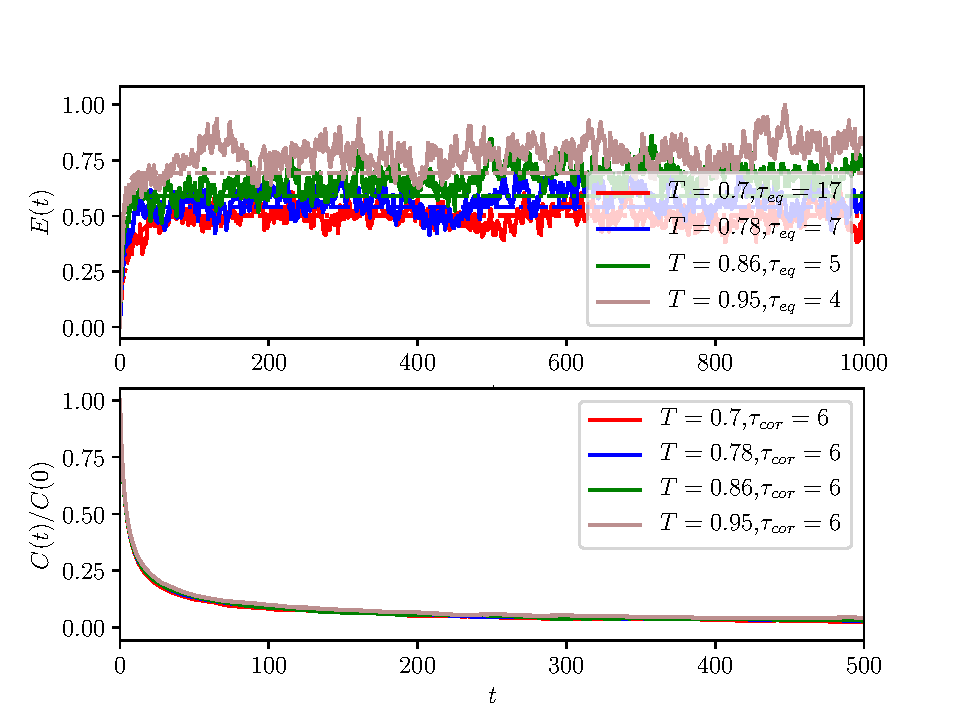
\includegraphics[scale=1]{numerical/sos-glau-eq-cor.pdf}
\caption{Plot of the energy per site (top) and the autocorrelation function (bottom) with Glauber dynamics from an initial state where $h_i=0$, for different temperatures.}
\label{eq-glau}
\includegraphics[scale=0.5]{example-image-a}
\caption{Mean height value per site with respect to $\mu$ different system size $L$ both by Glauber dynamics and diagonalization of the transfer matrix.}
\label{eq-glau} 
\end{figure}
The energy difference between two configurations is
\begin{align}
	\Delta E &= |h_{i-1}-(h_i + \alpha)| + |h_{i+1}-(h_i + \alpha)| - |h_{i-1}-h_i| - |h_{i+1}-h_i|  
\end{align}
It is not needed to compute the total height at each time step. We can stock $\sum_i h_i$ in a variable that is updated each time a transition is accepted by
\begin{align}
    <h>_{M+1} = <h>_M + \alpha
\end{align}
We can do the same for $\sum_i h_i^2$, which gives us the interface's width, or the total energy of the system with $\sum_i |h_i - h_{i+1}$.

In order to accelerate the equilibration process, we can directly start from the total height computed by the transfer matrix. We then get the equilibrium time by looking at $E(t)$. It is better practice to choose study the equilibration time by taking the total energy instead of the magnetization, since without external potential, the interface is delocalised and magnetization is only bounded by the boundary conditions. In Fig \ref{eq-glau}, we show the energy with respect to time and the autocorrelation function of the system in absence of chemical potential from a ground state $h_i=0$ for all $i$. The very small correlation and equilibration times means that numerical simulations reach the equilibrium distribution after $10^3$ MC steps, and that only $10^7$ MC steps will give accurate results.

In the SOS model, we expect to have the results from the Glauber dynamics to be exactly the same as the transfer matrix method, as shown in Fig \ref{tm-mc-equalt}, Since we can get exact results from the transfer matrix, the Glauber dynamics presents little interest for SOS models in the grand-canonical ensemble. Nevertheless, because there does not exist a transfer matrix formulation of the canonical ensemble, Monte Carlo simulations become interesting.

%%%%%%%%%%%%%%
\subsection{Kawasaki dynamics}
%%%%%%%%%%%%%%

Now we would like to have an algorithm for the canonical ensemble, where the total height stays constant. In the Kawasaki's algorithm \cite{kawasaki_diffusion_1966}, we randomly choose a site $i$ with probability $\frac{1}{L'}$, and one of its two neares neighboors $i-1$ or $i+1$ with probability $\frac{1}{2}$. For example, if we take the neighboor site $i-1$ (it holds the same for the site $i+1$), we generate a new configuration with Hamiltonian $H(h_0,...,h_{i-1}+1,h_i-1,...h_{L'})$, where we have taken a particle from site $i$ to diffuse it to the other site.
The selection probability is
\begin{align}
g(C\to C') = \frac{1}{2L'}
\end{align}
We also chose the same acceptance rate as in Glauber's dynamics \eqref{taux-transition-metropolis}.

Here, the total height is obviously conserved. In the case that we transfer a particle to site $i$ to site $i+1$, the energy difference is
\begin{align}
\Delta E &= |h_{i-1}-(h_i - 1)| + |h_{i+1} + 1 -(h_i- 1)| + |h_{i+1} + 1-(h_{i+2} )| \nn
& - \left( |h_{i-1}-h_i| + |h_{i+1} -h_i| + |h_{i+1}-h_{i+2}| \right)
\end{align}

\begin{figure}[t]
\centering
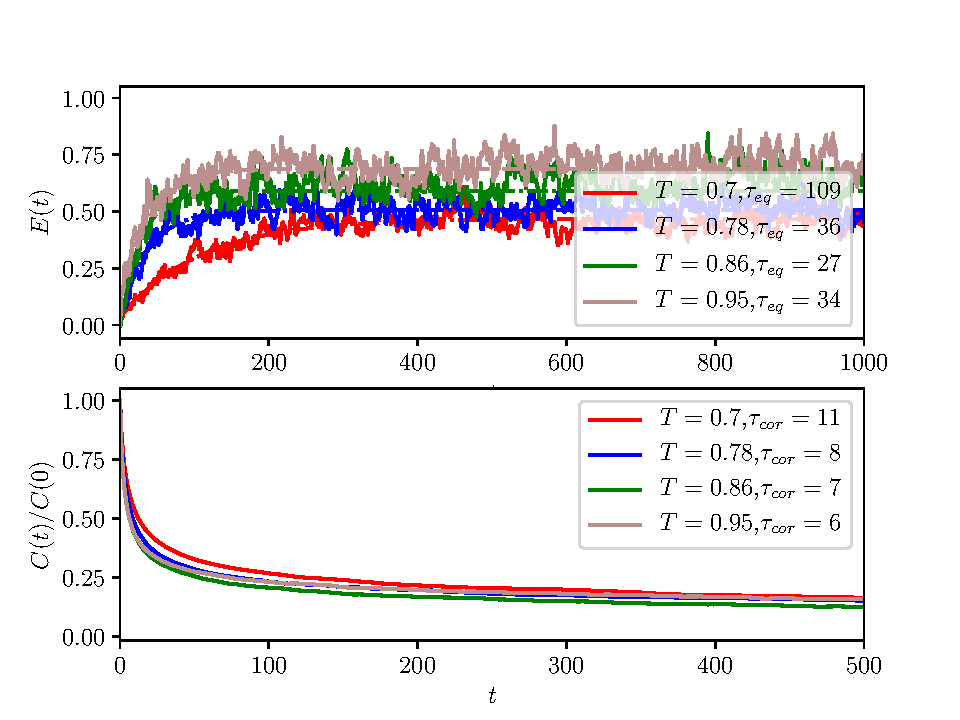
\includegraphics[scale=1]{numerical/sos-kaw-eq-cor.pdf}
\caption{Plot of the energy per site (top) and the autocorrelation function (bottom) with Kawasaki dynamics from an initial state where $h_i=0$, for different temperatures.}
\label{eq-kaw}
\end{figure}
In Fig \ref{eq-kaw}, we remark that both the equilibration and the correlation time are larger than for non-conserved dynamics, which is normal since the correlation length during coarsening goas as $t^\frac{1}{2}$ in model A and as $t^\frac{1}{3}$ in model B. Nevertheless they are of the same order of magnitude, which means that numerical simulations will take the same CPU time.

This dynamic describes the diffusion of particles at the interface. It is thus possible to add some hydrodynamic flow which breaks equilibrium. Since we have supposed that our configurations obeys the Gibbs-Boltzmann distribution, the Metropolis method stays pertinent if we assume that the dynamic is slow compared to the heat exchange with the reservoir.

%%%%%%%%%%%%%%%%%%% 
\section{Computing size dependent free energy}
%%%%%%%%%%%%%%%%%%% 

%%%%%%%%%%%%%%%%%%% 
\subsection{The Layer method}
%%%%%%%%%%%%%%%%%%%  

\begin{figure}
\begin{minipage}[t]{0.32\linewidth}
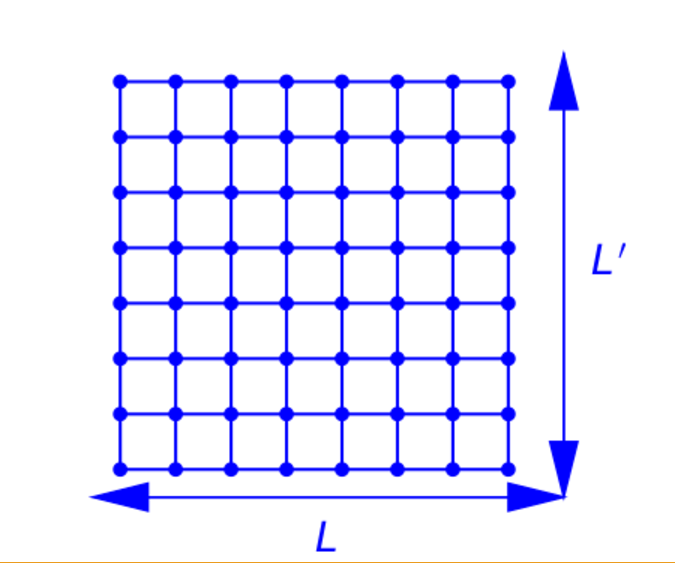
\includegraphics[width=\linewidth]{numerical/cross-h0.pdf}
\caption*{$H_0$}
\end{minipage}
\begin{minipage}[t]{0.32\linewidth}
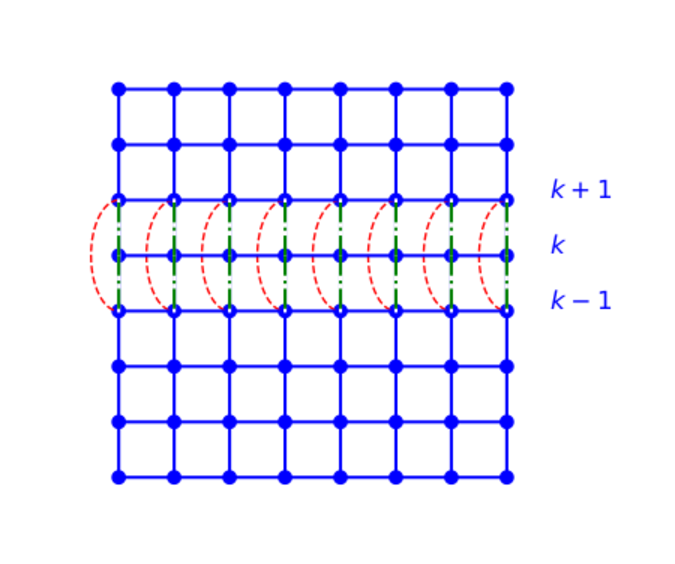
\includegraphics[width=\linewidth]{numerical/cross-hlambda.pdf}
\caption*{$H(\lambda)$} 
\end{minipage}
\centering
\begin{minipage}[t]{0.32\linewidth}
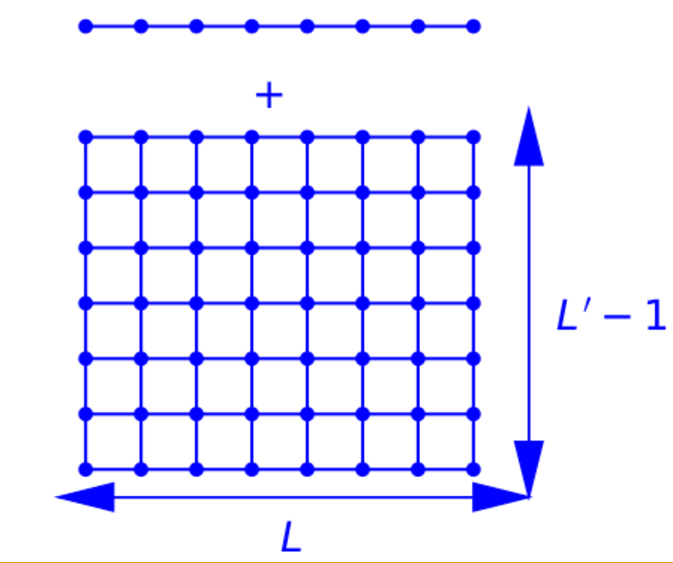
\includegraphics[width=\linewidth]{numerical/cross-h1.pdf}
\caption*{$H_1$}
\end{minipage}
\caption{Progessive decoupling of the $k$-th layer of the system in order to compute the freen energy through the Crossover Hamiltonian. Blue bonds have an energy of $\beta J$, red ones an energy of $\lambda \beta J $ and the green ones an energy of$ (1-\lambda) \beta J$. Reproduction 2D of \cite{ vasilyev_universal_2009}.}
\label{decouplage}
\end{figure}

It is not possible to compute from Monte Carlo simulations the free energy of a system, since it is not a derivative of the partition function. However, we can compute its derivative with respect to the system. This is useful to compute the Casimir force 
\begin{align}
F(t,h,L) = - \frac{\partial \Omega}{\partial L}
\label{casmir-mc}
\end{align}
To achieve that, Vasilyec \cite{vasilyev_universal_2009} developed a method to compute this derivative thanks to a dummy coupling parameter. Even though the system's size is discrete, it is possible to obtain a continuous-like size of the system thanks to the progressive decoupling the $k$-th layer of the system. If $H_0$ is the Hamiltonian of size $L$ and $H_1$ the Hamiltonian of size $L-1$ (see Fig \ref{decouplage}), then we define the crossover Hamiltonian as
\begin{align}
H_{cr}(\lambda) = (1-\lambda) H_0 + \lambda H_1
\label{hamil-trans}
\end{align}
with $\lambda \in [0,1]$, which interpolates from $H_0$ to $H_1$ when $\lambda$ goes from $0$ to $1$. As $\lambda$ goes on, we gradually decouple the $k$-th layer of the system, which means that the interaction energy of all vertical bonds between layer $k$ and layers $k-1$ and $k+1$ are now equal to $(1-\lambda)\beta J$, while we gradually couple the layers $k+1$ and $k-1$ with an energy $\lambda \beta J$.
The crossover Hamitlonian $H_{tr}(\lambda)$ also depends from the position of the decoupled layer $k \in {1,2,...,L}$ . The free energy associated to this system is
\begin{align}
\Omega_{cr}(\lambda) = -k_B T \ln \left( \sum_{h_1 ... h_L} \exp(-\beta H_{tr}(\lambda)) \right)
\end{align}
From the derivative of the free energy with respect to $\lambda$, we find
\begin{align}
\frac{\Omega_{cr}(\lambda)}{d\lambda} = < H_1 - H_0>_{H_{cr}(\lambda)}
\end{align}
where $< \cdot >_{H_{cr}(\lambda)}$ represents the statistical mean value in the crossover system, easily computable in numerical simulations. By integrating over the coupling constant, we have
\begin{align}
\Omega_1 - \Omega_0 = \int_0^1 d\lambda < H_1 - H_0>_{H_{cr}(\lambda)}
\end{align}
Finally, in the thick limit where $L\gg1$, we find
\begin{align}
- \frac{\partial \Omega(t,h,L)}{\partial L} \simeq \int_0^1 d\lambda < H_1 - H_0>_{H_{cr}(\lambda)}
\end{align}
Even though $H_{cr}(\lambda)$ depends of which layer we decided to decouple, and by transition $H_1-H_0$ and $< H_1 - H_0>_{H_{cr}(\lambda)}$, the integrand $\int_0^1 d\lambda < H_1 - H_0>_{H_{tr}(\lambda)}$ should be independent of this choice, as long as boundary conditions are not affect by the $k$-th layer.

For the SOS model, it is possible to exactly compute the energy variation produced by the decoupling. We find that
\begin{align}
&H_{cr,SOS}(\lambda) = H_{0,SOS} - \nn
&\frac{\lambda J}{2} \sum_x \left[ \sgn(k-1-h(x)) \sgn(k+1-h(x)) - \sgn(k-h(x)) \left( \sgn(k-1-h(x))+\sgn(k+1-h(x)) \right) \right]
\end{align}
where the prefactor $\frac{1}{2}$ take into account the prefactor between Ising and SOS models in Hamiltonian \eqref{energie-sos-ising}. By doing the ?? {\color{red} how do you translate "tableau de valeurs" ? } , we notice that every term in the sum is equal to $-1$ independently of $k$, since contrary to Ising models, SOS models do not possess any bulk energy. We 

%%%%%%%%%%%%%%%%%%% 
\subsection{The Lopes Cardozo method}
%%%%%%%%%%%%%%%%%%% 
Since the Layer method does not work for our models, we have to look to other ways. In the case of a chemical potential conjugated with the total height, we see that \cite{lopes_cardozo_critical_2014}
\begin{align}
<\sum_i h_i>(\mu,L) = - \frac{\delta \Omega(\mu,L)}{\delta \mu}
\end{align} 
If we integrate over the chemical potential, we have
\begin{align}
\Delta \Omega(\mu_1,\mu_2) = \Omega(\mu_1,L) - \Omega(\mu_2,L) = - \int_{\mu_1}^{\mu_2} <\sum_i h_i>(\mu,L) dh
\label{integration-cardozo}
\end{align}
In the case where we know the analytical forme of the free energy in the limits $\mu_2 \to \infty$ or $\mu_1 \to 0$, this method provides a way to directly measure the free energy of the system for any temperature or size by integrating over the chemical potential.

In the limit $\mu_2 \to \infty$, the correlation length at the reference state will be small so that the reference free energy will be essentially that of the bulk. As a consequence, it should contain all the information of the Casimir force \eqref{casmir-mc}. That derivative force can then be computed by 
\begin{align}
\delta L \frac{\partial \Omega(\mu_1,L)}{\partial L} = \Delta \Omega(\mu_1,\mu_2,L)-\Delta \Omega(\mu_1,\mu_2,L-\delta L)
\end{align}
where $\delta L$ is the difference thickness between two systems, and which is then independent of $\mu_2$ in the large chemical potential limit as the free energy $\Omega(\mu_2,L)$ converges to the bulk energy.

Since in Kawasaki dynamics the total height is constant, this method does work only for model A.

%%%%%%%%%%%%%%%%%%% 
\section{Tips and tricks}
%%%%%%%%%%%%%%%%%%% 

The simulation's speed of SOS models is so great compared to Ising ones that it is possible to study systems over a wider range of parameters. A SOS simulation of $10^7$ MC steps takes roughly 20 minutes to complete once fully optimized. We see that if we want to launch hundreds of those simulations, it can easily take days, which forces us to optimize the code.
In C++, if compiling with g++, the first thing to do is to compile the programme with the $-O3$ flag, which makes you gain an order of magnitude in CPU time.

The most important part of Monte Carlo simulations are the pseudo Random Number Generator (pRNG), which are called at least twice for each transition attempt. The C++ standard library proposes the function \textit{default\_random\_engine} as the default pRNG. A lot of CPU time can be saved by switching to \textit{sfc64} or \textit{xoroshiro} pRNGs. Furthemore, the generation of $\pm1$ numbers only require one bit, while the pRNG always generates a 64-bits number, thus wasting 63-bits at each boolean generation. A wasteless method which speeds considerably the simulation's speed can be found in \cite{martin_ankerl_fast_nodate}.

Lastly, the easiest way to gain real time is to make the code parallel. We can do that either by domain decomposition - which would allow us to simulate larger systems - or parallelise directly over the simulation's parameters (as the temperature or the chemical potential). While the first one is useless in SOS model because of the short correlation length of such systems, the latter can be done via two libraries : OpenMP and MPI. It took me some time to understand that the memory-shared OpenMP protocol has a lot of problems with pRNGs, making this library not suited for Monte Carlo simulations. On the contrary, the MPI library provides impermeability between threads, which makes it the better choice.

%%%%%%%%%%%%%%%%%%%%%%%%%%%%%%%%%%
\section{Conclusion}
%%%%%%%%%%%%%%%%%%%%%%%%%%%%%%%%%%

In this chapter, we have explained how to compute expectation values of observables in our system, thanks to the Monte Carlo Metropolis algorithm. For that, we need to suppose that the system is in thermal equilibrium with a heat bath, and that it respects detailed balance. We have two different possible algorithms : the Glauber dynamics allows to study the systems in the grand-canonical ensemble, while the Kawasaki dynamics is for canonical ones. Nevertheless, since the transfer matrix method gives exact results for the grand-canonical ensemble, only the Kawasaki dynamics is relevant for SOS models. 

In addition to that, measuring the free energy of the system is not an easy task, as we can only compute its derivative. The first method we have presented is about progressively decoupling a layer of the system, even though for SOS models, which do not possess a bulk energy, the method does not work. Another method is to integrate over the conjugate variable coupled to the total height, which is the chemical potential. This method does not work for Kawasaki algorithms. 
Since as we have discussed Glauber simulations are not relevant for our models, we find that we have no way to compute the free energy in Monte Carlo methods for the only relevant ensemble which is the canonical one. In a latter chapter, we will see how to fix this issue.
\chapter{Résultats pour le modèle SOS}
    \label{chap-sos}

On considère un système de longueur $L$ et de hauteur $N$. Pour $N$ très grand, si la position de l'interface est loin de $0$ ou de $N$, on s'attend à retrouver toutes les propriétés d'un modèle infini centré en 0. Si l'interface est proche de $0$, on pourra étudier les effets au bord, comme dans un système semi-infini\footnote{Dans les simulations numériques ainsi que pour la diagonalisation des matrices nous sommes obligés de choisir une taille finie de notre système. Cependant l'équivalence avec les calculs analytiques dans les sytèmes (semi)infinis mest vraie pour de grandes tailles de systèmes}.  On fixe la hauteur moyenne $<h_i> = H$ grâce au potentiel chimique $\mu$\footnote{Calculer la magnétisation moyenne via des librairies comme \hyperlink{http://eigen.tuxfamily.org/index.php?title=Main_Page}{\underline{Eigen en C++}} (contrairement à la librairie GSL plus difficile d'accès) permet d'accélérer grandement l'étape d'équilibrage du système pour le Monte Carlo.}.

\begin{figure}[h]
	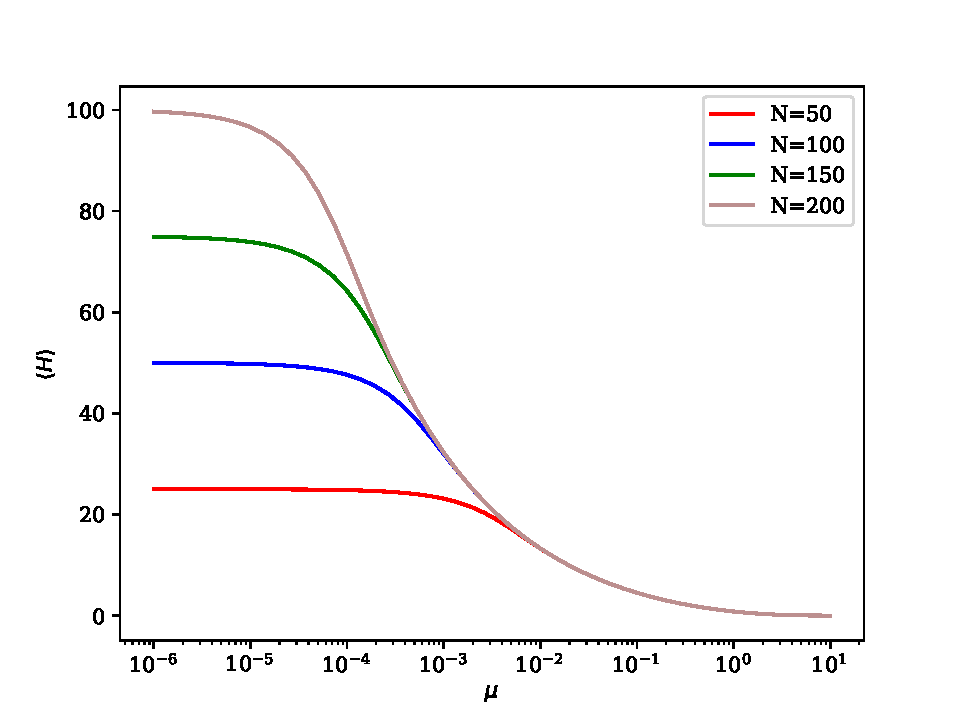
\includegraphics[width=\linewidth]{semiifgeom/hauteur-mu.pdf}
	\caption{Hauteur moyenne de l'hamiltonien $H = \sum_i |h_i-h_{i+1}| + \mu \frac{h_i+h_{i+1}}{2}$ en fonction de $\mu$ calculée grâce à la diagonalisation d'une matrice de transfert de taille $N$. Lorsque le potentiel chimique est trop faible, l'interface est délocalisée et se retrouve à la position $\frac{N}{2}$. }
	\label{hauteur-mu}
\end{figure}

	\section{Différences Glauber/Kawasaki}

figure énergie moyenne, sigma, distribution de probabilité via Airy	
	
	\section{Effet du cisaillement}

Dans les expériences, le système est soumis à un cisaillement au niveau de l'interface, ce qui modifie les observables par rapport à l'état d'équilibre. Nous optons ici pour un modèle de cisaillement uniforme dont le sens est défini par $\sgn(i-j)$, $i$ et $j$ étant des sites de hauteurs respectives $h_i$ et $h_j$. 
La différence d'énergie entre un micro-état et le suivant d'une étape de Monte Carlo sous une dynamique de diffusion (Kawasaki) est alors
\begin{align}
	\Delta E = J \sum_i \left[ |h'_i-h'_{i+1}|-|h_i-h_{i+1}| \right] \pm f 
\end{align}
où $h_i'(t) = h_i(t+1)$ - le temps étant discrétisé, $f$ le module de cisaillement et le signe du cisaillement étant pris de manière aléatoire à chaque étape, regardant ainsi si ce mouvement va dans ou contre le sens du flux. 

Pour rappel, à chaque étape on essaie de transférer une particule du site $i$ vers son voisin (gauche ou droit) $j$, ce qui se traduit par $h_i' = h_i-1$ et $h_j' = h_j+1$. 
Pour $f=0$, en remarquant que les valeurs absolues ont les propriétés suivantes
\begin{align}
	|a \pm 1| - |a| = \pm 1 \\
	|a \pm 2| - |a| = {0,\pm 2}
\end{align}
nous voyons facilement l'émergence d'une sélection des énergies possibles entre deux micro-états successifs dans ${-4,-2,0,2,4}$. Ainsi, toutes les transformations diminuant l'énergie totale du système seront toujours acceptées. En augmentant le cisaillement il devient alors possible de refuser des états réduisant l'énergie et d'accepter ceux qui l'augmente. 
Nous nous attendons alors à trois régimes différents :
\begin{itemize}
	\item $f  \less  2 J $ : à faible cisaillement, la symmétrie du système impose les observables à être paire vis-à-vis de $f$, comme le prouve le fit en carré des figures.
	\item $2 J \less f \less 4 J$ : à cisaillement moyen, certains mouvements augmentant la rugosité de l'interface sont toujours acceptés. 
	\item $f > 4 J$ : à haut cisaillement, tous les mouvements augmentant l'entropie du système sont acceptés. Une saturation du système se produit lorsque l'énergie de lien entre les sites devient négligeable face au cisaillement.
\end{itemize}


\begin{figure}[h]
	\includegraphics[width=\linewidth]{./semiifgeom/sosj1.pdf}
	\caption{Énergie $E= \langle \sum_i |h_i-h_i+1| \rangle$ (en pointillé sa dérivée), variance $\sigma = \langle (H - \langle H \rangle )^2  \rangle$ et asymétrie $\gamma = \langle (H - \langle H \rangle )^3  \rangle / \sigma^2$ pour $B^0.1$. La magnétisation est constante et égale à $\langle H \rangle = 4.51$. Le temps de corrélation du système est presque constant en fonction du cisaillement $f$, allant de  $\tau(f=0) = 5.04$ à $\tau(f=6) = 5.00$ étapes de Monte Carlo. On note une brisure à $f=2J$ et $f=4J$.
Les croix notent un fit en carré pour petit $f$, montrant la symétrie du système par inversion du signe de $f$. }
\end{figure}

\begin{figure}
	\includegraphics[width=\linewidth]{./semiifgeom/j13.pdf}
	\caption{Same as before, with $J=1.3$ We observe a net inflexion in the energy at $2 J$ for  $B=0.01$ which corresponds to $<H>=11$. Nvertheless there is not threshold at $4 J = 5.2$. My guess is that the system is too far away from the boundary in order to interact strongly with it. Interstingly enough, for $B=0.1$, $<H>=3$ and we are too close to the boundaries to see anything.}
\end{figure}

	\subsection{Différences avec le modèle d'Ising}

	Le modèle d'Ising repose sur la perméabilité entre les deux phases, avec des bulles d'une phase dans l'autre. Dans les travaux sur le rôle du cisaillement au niveau de l'interface dans un modèle d'Ising ( \cite{smith_driven_2010},\cite{smith_interfaces_2008}. ), le cisaillement s'applique à toutes les particules, ce qui a pour but d'étirer les bulles, les rendant plus fragiles au bain thermique. Cet effet participe à leur évaporation vers l'interface et à la dissipation de l'énergie injectée par le cisaillement.
	
	Au contraire, dans les modèles que nous utilisons ici, où l'interface peut fluctuer mais est imperméable, l'énergie injectée au niveau de l'interface ne peut être dissipée par évaporation, ce qui conduit à l'émergence d'une phénoménologie différente. Il est ainsi impossible de définir un cisaillement qui soit appliqué à l'intérieur des phases, puisqu'il n'existe aucune notion de particules. Plus loin nous développons un modèle qui s'abstrait de ces difficultés. 


\section{Cisaillement avec deux types de particules}

La construction naïve d'un modèle continu du cisaillement avec un seul type de particules ne donnera aucun résultat. En effet, pour que le cisaillement induise des effets hors équilibre, il faut que la dynamique des particules dans tout repère galilén soit le même. Si l'on considère une force de cisaillement uniforme qui induit la même vitesse moyenne sur toutes les particules du système, en nous plaçant dans un repère bougeant à la même vitesse que cette vitesse moyenne, nous retrouvons les mêmes propriétés à l'équilibre.
Afin de briser la symmétrie de translation, il faut soit induire un cisaillement non-uniforme, soit introduire des particules qui réagissent de manière différente vis-à-vis de cette force. Dans notre exemple sur les colloïdes, la gravité agit bien sur les polymères mais bien moins sur le solvant, ce qui brise en effet l'invariance galiléenne. 
Plusieurs études récentes portent sur le mouvement de systèmes avec plusieurs particules browniennes\cite{netz2003,dzub2002,chak2003,chak2004,lowe2009,glan2012, klym2016}, incluant le problème des électrolytes étudié par Onsager \cite{onsager} il y a longtemps.

	\subsection{Discussion about the Gaussian model}
	
The Gaussian model has a stronger interaction, been as
\begin{align}
	\Delta E = J \sum (h'_i-h'_{i+1})^2 -(h_i-h_{i+1})^2+ f (i-j)
\end{align}
In this model the bond energy between two microstates can take any integer, as 
\begin{equation*}
	(h_i-h_j+2)^2 - (h_i-h_j)^2 = 4 (h_i-h_j+1)
\end{equation*}

The gaussian interaction is very strong, so we could expect a very smooth interface. The mean difference between two sites should be about $h_i-h_{i+1} \simeq 1$. In that case, the energy difference is discretized as ${-8,-4,0,4,8}$. 
Nonetheless we cannot predict exactly the same behaviour as in the SOS model because this approximation has to be verified everytime, which is false. 1

\begin{figure}
	\includegraphics[width=\linewidth]{./semiifgeom/gauss0.pdf}
	\caption{Bond energy, thickness (variance) and skewness of the interface for two different magnetic pressures. The magnetisation is constant and is equal to $<H>=2$ for $B=0.1$. As we are very close to the boundary, we see no threshold with the drive force. Simulations take longer with this model because the interaction is stronger}
\end{figure}

	\section{Interpretation}
	
	
\chapter{Champ magnétique $|h_i|$}
\label{sec_laser}

Certains systèmes qui favorisent une espèce de particules d'un côté de l'interface et une autre espèce de l'autre côté se retrouvent dans plusieurs expériences, par exemple une croissance de cristaux contrôlée par un champ optique\cite{} ou le forçage d'une phase dans une autre dans des expériences d'optofluidique\cite{delville}. Ces systèmes ont la particularité d'avoir une singularité dans le champ magnétique au niveau de l'interface, du genre 
\begin{align}
	B(y) = B \sgn(y)
\end{align}
 où l'interface est placée convenablement en $0$ et $B$ est l'intensité du champ magnétique. Dans le formalisme SOS, ce champ magnétique se traduit par 
\begin{align}
	B(h_i) = B |h_i|
\end{align}
Pour $B>0$, le potentiel a un minimum absolu en $0$, confinant ainsi l'interface. On s'attend à ce que plus le champ magnétique devienne élevé, plus l'interface devienne confinée. 

Nous discuterons brièvement à la fin du chapitre le cas où $B$ est négatif.


	\section{Modèle gaussien}

Un potentiel aussi complexe présente de nombreuses difficultés pour la diagonalisation. Une des difficultés provient du grand nombre de degrés de liberté du système. Afin de diminuer la complexité du calcul, supposons que l'interface soit continue, c'est-à-dire que l'interface au point $x$ soit notée $h(x)$. Cette interface n'est plus définie uniquement aux sites discrets $i$, puisque l'on s'intéresse aux propriétés mésoscopiques du système.

L'énergie du modèle SOS est directement dictée par $E = \sigma \mathcal{L}$, où $\sigma$ est la tension superficielle de notre interface et $\mathcal{L}$ la longueur totale de notre interface. Cette longueur correspond à la distance parcourue par un marcheur brownien le long de l'interface dans des conditions en $x$ périodiques. D'un point de vue continu, la distance effectuée pour de petits déplacements est $d\mathcal(L) = \sqrt{1+\frac{dh^2}{dx^2}} \simeq h'^2 $.
L'Hamiltonien discret correspondant devient gaussien
\begin{align}
    H = J \sum_i (h_i-h_{i+1})^2
\end{align}
tandis qu'une version continue du problème est 
\begin{align}
	H = \frac{\sigma}{2} \int_0^L h'^2(x) dx - B \int_0^L |h(x)|dx
\end{align}
Cet hamiltonien gaussien est très similaire à celui que l'on peut retrouver pour les ondes capillaires\cite{} et facilite grandement les calculs. 

    \section{Distribution de l'interface}

Pour une interface avec des conditions aux bords fixe $h(0) = h$ et $h(L) = h^\ast$, la fonction de partition est donnée par
\begin{align}
	\mZ(h,h^\ast,L) = \int_{h(0)=h} d[h] \delta(h(L)-h^\ast)e^{-\frac{\sigma}{2} \int_0^L h'^2(x) dx + B \int_0^L |h(x)|dx}
\end{align}
La configuration de l'interface à un instant $t$ est similaire à celle de la trajectoire temporelle d'un marcheur brownien commençant à $h(0)$ et finissant à $h(L)$\cite{}.
La fonction de partition $\mZ$ obéit alors à l'équation de Schrödinger temporelle
\begin{align}
	\frac{\partial \mZ}{\partial L} = \frac{1}{2 \beta \sigma} \frac{\partial^2 \mZ}{\partial h^2}  - B \beta |h| \mZ
\end{align}
avec la condition initiale $\mZ(h,h',0) = \delta(h-h')$.  En absence d'un potentiel externe on retrouve les solutions en sinus et cosinus décrivant une interface délocalisée à travers tout le système. En décomposant la fonction de partition dans la base des solutions stationnaires $\psi_E$ correspondant aux énergies propres $E$ 
\begin{align}
	Z(h,h',L) = \sum_E e^{-EL}\psi_E(h)\psi_E(h')
	\label{schro_temp}
\end{align}
À nouveau, dans la limite thermodynamique, seul l'état fondamental $E_0$ contribue à la distribution des hauteurs $p(h) = \psi_{E_0}^2(h)$.
Chaque fonction propre obéit alors à l'équation de Schrödinger 
\begin{align}
	\epsilon \psi_\epsilon = - \frac{1}{2} \frac{\partial^2 \psi_\epsilon}{\partial h^2} + \lambda |h| \psi_\epsilon
\end{align}
où l'équation a été admiensionalisée par $\epsilon = E\beta\sigma$ et $\lambda=\beta^2 \sigma B$.
Les solutions sont données par les fonctions d'ondes paires
\begin{align}
	\psi_\epsilon (h) = Ai \left( (2\lambda)^\frac{1}{3}|h|-\frac{\epsilon}{\lambda} \right)
\end{align}


où $Ai(x)$ est la fonction de Airy. Par analogie avec l'oscillateur harmonique quantique, nous cherchons des solutions avec des conditions aux limites $\psi'_\epsilon(0) = 0$ pour les états pairs et $\psi_\epsilon(0) = 0$ pour les états impairs. Cela nous donne $\epsilon_n = 2^{-\frac{1}{3}} \lambda^\frac{2}{3}\alpha_n$ où $-\alpha_{2n} \greater 0$ est le 2n-ième zéro de la dérivée de la fonction d'Airy Ai' et $-\alpha_{2n+1} \greater 0$ est le (2n+1)-ième zéro de la fonction d'Airy Ai. L'état fondamental est donné par le plus petit zéro de la fonction $\alpha_0 = 1.0187..$ et a une énergie de 
\begin{align}
	E_0 = 2^{-\frac{1}{3}} \alpha_0 \beta^\frac{1}{3}\sigma^{\frac{1}{3}}B^\frac{2}{3}
\end{align}
L'état fondamental s'écrit alors
\begin{align}
	\psi_0(h) = \frac{ Ai ( (2\lambda)^\frac{1}{3} |h|-\alpha_0 )}{ \sqrt{2 \int_0^\infty dh Ai^2 ( (2\lambda)^\frac{1}{3} |h|-\alpha_0 ) }}
\end{align}
où le terme d'en bas est une constante de normalisation utilisant la symétrie $p(h)=p(-h)$.  
On peut calculer les états excités suivants suivant leur parité, les états pairs s'écrivant
\begin{align}
	\psi_{2n}(h) = \frac{ Ai ( (2\lambda)^\frac{1}{3} |h|-\alpha_{2n} )}{ \sqrt{2 \int_0^\infty dh Ai^2 ( (2\lambda)^\frac{1}{3} h-\alpha_{2n} ) }}
\end{align}
et les états impairs
\begin{align}
	\psi_{2n+1}(h) = \frac{ \sgn(h) Ai ( (2\lambda)^\frac{1}{3} |h|-\alpha_{2n+1} )}{ \sqrt{2 \int_0^\infty dh Ai^2 ( (2\lambda)^\frac{1}{3} h-\alpha_{2n+1} ) }}
\end{align}
d'énergie $E_{n} = E_0 \frac{\alpha_{n}}{\alpha_0}$. 

\begin{figure}[h]
	\begin{minipage}[t]{0.5\linewidth}
        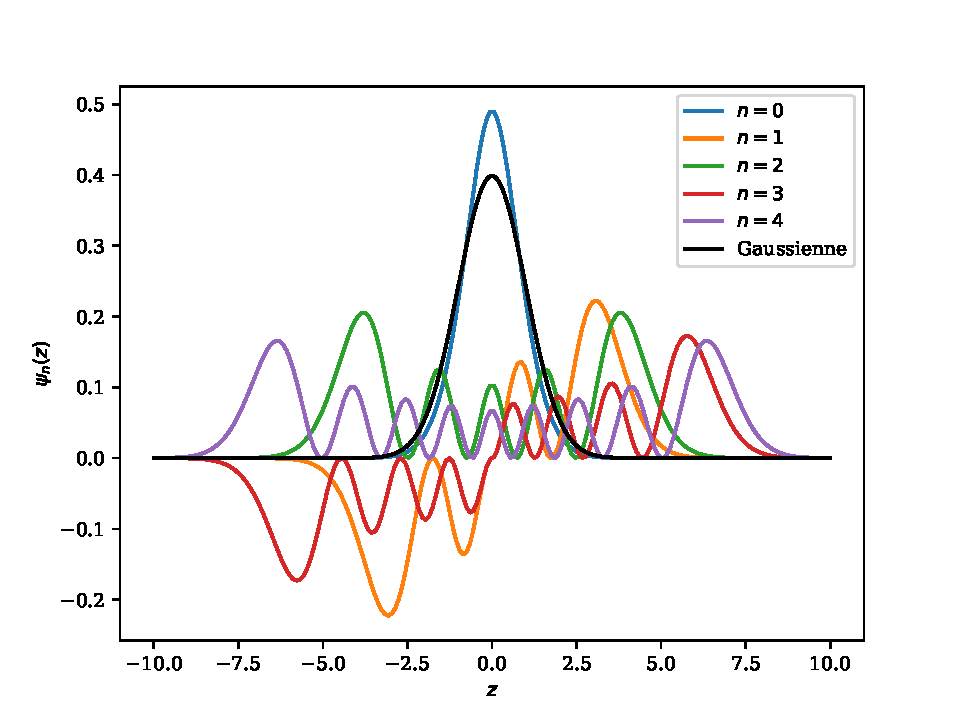
\includegraphics[width=\linewidth]{sosequi-laser/etats-laser.pdf}
	\end{minipage}%
	\begin{minipage}[t]{0.5\linewidth}
    	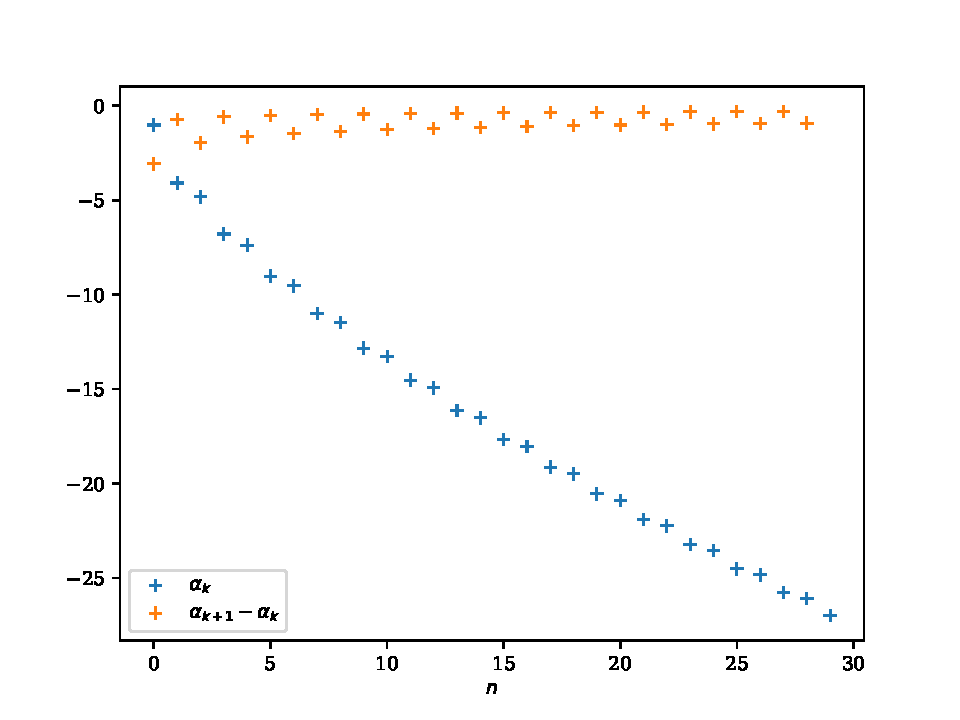
\includegraphics[width=\linewidth]{sosequi-laser/energies-laser.pdf}
	\end{minipage}
    \caption{À gauche, états propres $\psi_n$ avec en noir, une référence par rapport à la distribution gaussienne. À droite, la série $\alpha_n$.}
\end{figure}



On peut adimensionner la distribution des hauteurs par $z = (2\lambda)^\frac{1}{3}h$, et on peut définir une largeur caractéristique de l'interface 
\begin{align}
	\xi_\perp = \frac{1}{(2\beta^2 \sigma B)^\frac{1}{3}}
	\label{xi_perp}
\end{align}


La distribution des hauteurs dans un système infini devient 
\begin{align}
	p(z) = \psi_0^2(z) = \frac{ Ai^2 ( |z|-\alpha_0 )}{ 2 \int_0^\infty dz Ai^2 ( z-\alpha_0 ) }
	\label{airy}
\end{align}
	
\begin{figure}[h]
	\begin{minipage}[t]{0.5\linewidth}
		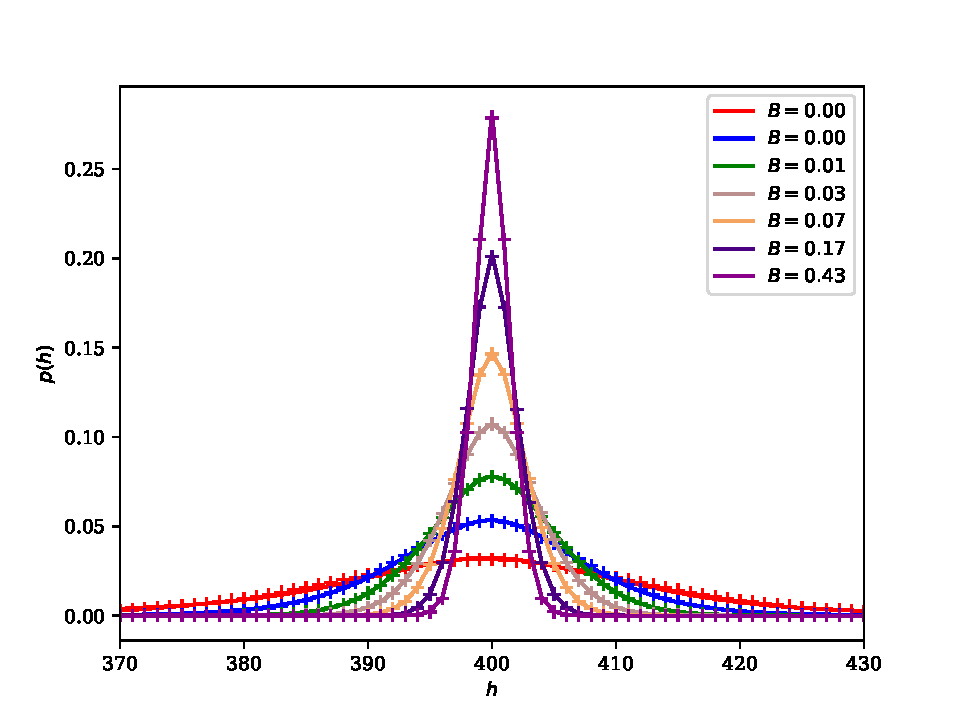
\includegraphics[width=\linewidth]{sosequi-laser/histo.pdf}
	\end{minipage}%
	\begin{minipage}[t]{0.5\linewidth}
		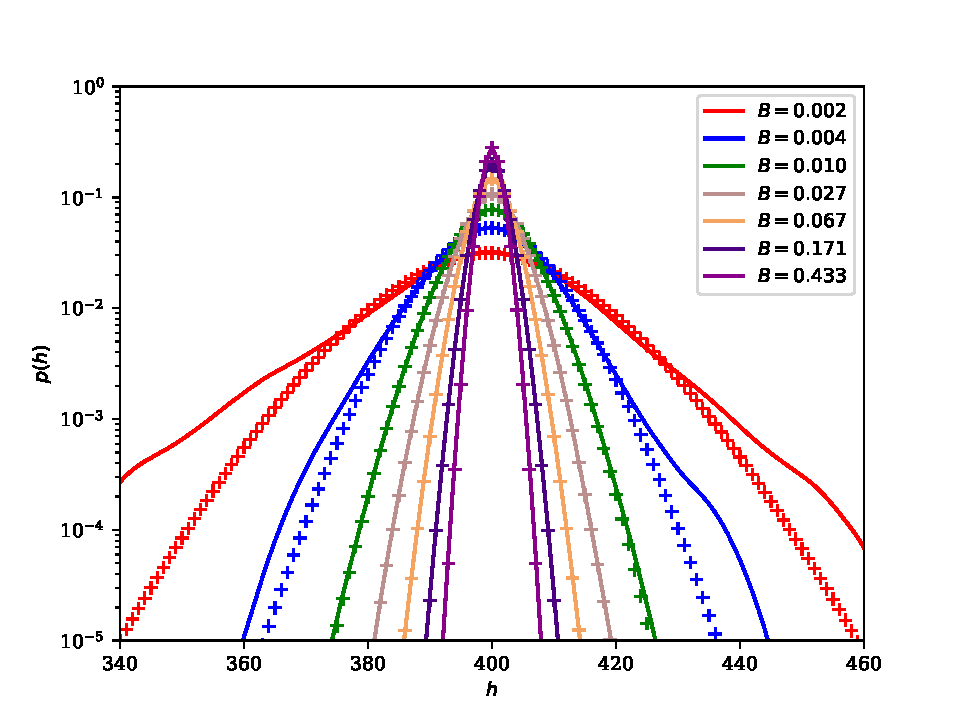
\includegraphics[width=\linewidth]{sosequi-laser/loghisto.pdf}
	\end{minipage}
	\caption{ Distribution de l'interface à $\beta = \beta_C$ autour d'un système centré à $L_Y=400$ en ligne et un fit selon la distribution de Airy \ref{airy}\protect\footnotemark en croix en échelle normale (à gauche) et en échelle log (à droite). Les écarts aux grandes fluctuations sont dues à un temps d’échantillonnage trop faible ($10^8$ MC steps) par rapport au temps de corrélation ($T_{cor} \simeq 100$), ce qui ne donne qu'environ $10^6$ états décorrélés. Par comparaison, à haut champ magnétique, le temps de corrélation est $T_{cor} \simeq 2$.  }
	\label{histo_airy}
\end{figure}

\footnotetext{En C++, les tableaux commençant par l'indice $0$, il est donc plus simple de centrer le système loin de $0$ afin de ne pas avoir à translater les variables à chaque fois. Par ailleurs, le fit est très sensible aux conditions initiales.}

\begin{figure}[h]
	\begin{minipage}[t]{0.5\linewidth}
		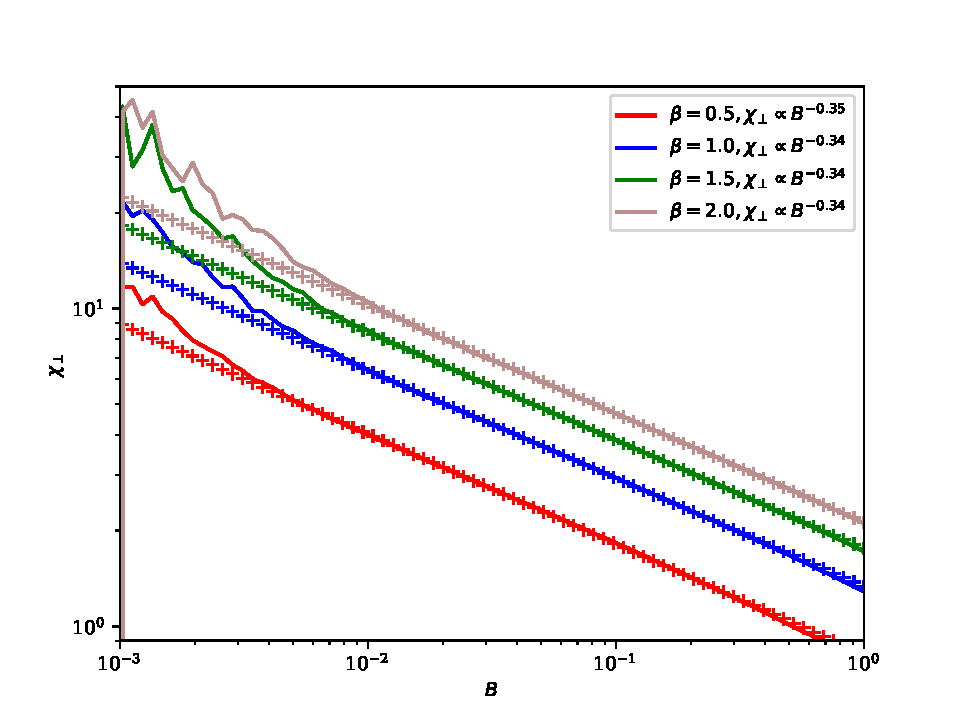
\includegraphics[width=\linewidth]{sosequi-laser/glau-chi.pdf}
	\end{minipage}%
	\begin{minipage}[t]{0.5\linewidth}
		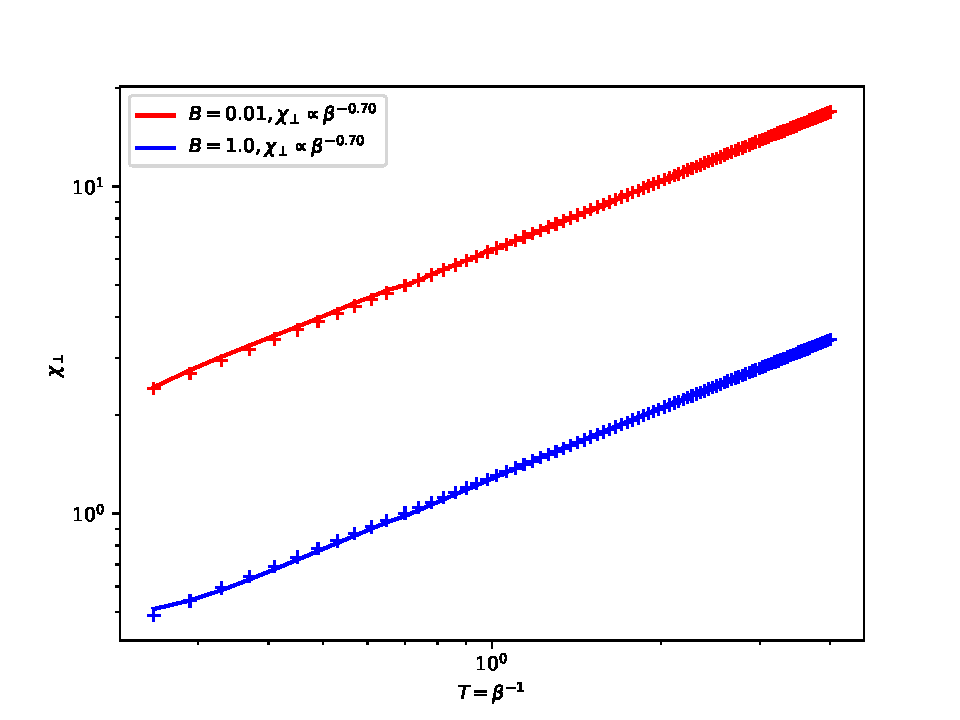
\includegraphics[width=\linewidth]{sosequi-laser/glau-chi-temp.pdf}
	\end{minipage}
	\caption{$\xi_\perp$ calculé via un fit de la distribution numérique par la distribution de Airy après $10^8$ MC steps (\ref{airy}) en fonction du champ magnétique et à température constante (gauche) ou en fonction de la température et à champ magnétique constant (droite). Les fluctuations pour $B$ petit s'expliquent par la difficulté d'équilibrage du système. On retrouve une loi en puissance comme dans l'équation \ref{xi_perp}.}
	\label{expo_airy}
\end{figure}

Comme montré précédemment, le calcul numérique de la distribution de l'interface nous permet d'avoir accès à  la tension de surface de notre modèle via la mesure de la longueur caractéristique $\xi_\perp$. Dans la figure \ref{histo_airy}, le fit de la distribution des hauteurs via l'équation \ref{airy} nous permet d'obtenir $\xi_\perp(\beta,B)$ de la figure \ref{expo_airy}. Ainsi, on obtient que 
\begin{align}
	\xi_\perp(\beta,B) \propto \beta^{-0.34} B^{-0.70} 
\end{align}

\textbf{Est-ce utile de faire une étude plus poussée sur plus de B et $\beta$ afin d'avoir une barre d'erreur sur les exposants ?}

Grâce aux calculs, il est possible d'inverser \ref{xi_perp} afin de trouver numériquement la tension superficielle du système. Dans le tableau \ref{tab_sigma}, en supposant un exposant en $\beta$ de $-0.70$, un tableau à titre informatif sur la tension de surface calculée en fonction de différents paramètres $T = \frac{1}{\beta}$ et $B$ grâce à l'équation \ref{xi_perp}. Les grandes fluctuations de $\sigma$ proviennent d'un échantillonage trop faible du calcul de l'exposant de $\beta$ et de $B$. De plus, d'après la figure \ref{expo_airy}, il semblerait que la loi en puissance ne soit pas valable dans tous les régimes, ce qui ajoute de l'incertitude à nos calculs.
Au final on constate que $\sigma \simeq 4.5$ dans notre modèle pour $J=1$. Des études plus approfondies utilisant la fonction de corrélation et $\xi_\parallel$ permettraient calculer précisément la tension superficielle dans le modèle SOS.

\begin{table}[h]
    \centering
$\begin{array}{|c|c|c|c|c|}
\hline
    T & B & \xi_\perp & \text{Exposant de B} &  \sigma \\
\hline
0.5 & 0.01 & 3.94 & -0.347 & 4.55 \\
0.5 & 1.0 & 0.78 & -0.347 & 4.01 \\
1.0 & 0.01 & 6.29 & -0.340 & 4.80 \\
1.0 & 1.0 & 1.28 & -0.340 & 4.23 \\
1.5 & 0.01 & 8.36 & -0.340 & 4.75 \\
1.5 & 1.0 & 1.72 & -0.340 & 4.36 \\
2.0 & 0.01 & 10.26 & -0.342 & 4.71 \\
2.0 & 1.0 & 2.11 & -0.342 & 4.37 \\
\hline
\end{array}$
    \caption{Meilleure estimation possible de la tension superficielle d'après les simulations numériques pour quelques valeurs de $T$ et de $B$.  }
    \label{tab_sigma}
\end{table}

    \section{Fonction de corrélation }

On peut également calculer la fonction de corrélation à deux-points. 
D'après l'éq \ref{schro_temp}, l'énergie de chaque état est une longueur caractéristique de chaque mode, $E_0$ étant la plus importante contribution au système. La longueur de corrélation parallèle à l'interface étant de l'ordre de grandeur de $E_0^{-1}$, on a 
\begin{align}
	\xi_\parallel = \frac{1}{E_0} =  2^\frac{1}{3}  \beta^{-\frac{1}{3}} \sigma^{-\frac{1}{3}}B^{-\frac{2}{3}}
\end{align}


Dans la limite thermodynamique $L$ grand, la fonction de corrélation  à l'interface est
\begin{align}
	C_f(r) &= \langle f(h(0))f(h(r))\rangle - <f(h(0))><f(h(r))>
\end{align}
Puisque nous sommes dans la limite thermodynamique, la fonction de partition devient $\mZ \simeq e^{-E_0 L}$ et $<f(h(0))> = <f(h(r))> = \int_{-\infty}^\infty dh f(h) \psi_0(h)^2 $.
On obtient alors que
\begin{align}
	C_f(r) =  \sum_{n\neq 0}\left[\int_{-\infty} ^\infty dh\  f(h)\psi_n(h)\psi_0(h)\right]^2\exp(-[\alpha_n-\alpha_0] \frac{r}{\xi_{||}})
\end{align}
En particulier, si
\begin{align}
	f(h) = {\rm sign}(h-y)
\end{align}
alors $C_f(r)=C(y,r)$ est la fonction de corrélation spin-spin mesurée parallèlement à l'interface à la hauteur $y$. On peut décomposer l'intégrale en deux parties, et grâce à un changement de variable obtenir
\begin{align}
	\int_{-\infty} ^\infty dh\  f(h)\psi_n(h)\psi_0(h)=  2\int_y ^\infty dh\  \psi_n(h)\psi_0(h)
\end{align}
Puisque les $\psi_n$ sont des fonctions d'onde orthogonales répondant à l'équation de Schrödinger, l'intégrale pour $n\neq 0$ est
\begin{align}
	I(n,y)&= \int_y^\infty dh\psi_n(h)\psi_0(h)  \nn
	&= \frac{1}{2}\frac{\psi_0(x)\psi'_n(y) - \psi_n(x)\psi_0'(y)}{\epsilon_n-\epsilon_0}
\end{align} 
Comme précédement, on notant $z= \frac{y}{\xi_\perp}$, on simplifie la fonction de corrélation en
\begin{align}
	C(z ,r) = \sum_{n\neq 0} \frac{\left[ Ai(|z|-\alpha_0)Ai'(|z|-\alpha_n) -Ai(|z|-\alpha_n)Ai'(|z|-\alpha_0) \right]^2}
{ \int_0^\infty dz Ai^2 ( z-\alpha_0 )2 \int_0^\infty dz Ai^2 ( z-\alpha_n ) (\alpha_n-\alpha_0)^2}e^{-[\alpha_n-\alpha_0] \frac{r}{\xi_{||}}}
\end{align}

La constante de normalisation peut être encore simplifiée. L'intégration par partie donne
\begin{align}
	N_n = \int_0^\infty dz Ai^2 (z -\alpha_n) = [z Ai^2 (z -\alpha_n)]_0^\infty - 2\int_0^\infty dz  z Ai(z -\alpha_n)Ai'(z -\alpha_n)
\end{align}
Le terme aux limites est nul, et en utilisant l'équation d'Airy 
\begin{align}
	Ai''(z) -z{\rm Ai}(z)=0 \implies z Ai(z-\alpha_n) = Ai''(z-\alpha_n) + \alpha_n Ai(z-\alpha_n)
\end{align}
on obtient
\begin{align}
	N_n &= -2\int_0^\infty dz [Ai''(z -\alpha_n)+\alpha_n Ai(z -\alpha_n)] Ai'(z -\alpha_n)  \nn
	&= Ai'^2(-\alpha_n) + \alpha_n Ai^2(-\alpha_n).
\end{align}

Cela nous donne au final
\begin{align}
	C(z,r) = \frac{1}{6.7 \times 10^{-3}}\sum_{n\neq 0} \frac{\left[ Ai(|z|-\alpha_0)Ai'(|z|-\alpha_n) -Ai(|z|-\alpha_n)Ai'(|z|-\alpha_0) \right]^2}
{(Ai'^2(-\alpha_n) + \alpha_n Ai^2(-\alpha_n))  (\alpha_n-\alpha_0)^2}e^{-[\alpha_n-\alpha_0] \frac{r}{\xi_{||}}}
\end{align}

À grande distance, seul le terme premier état excité $n=1$ contribue à la fonction de corrélation, ce qui nous donne
\begin{align}
C(x,r) \approx \frac{[{\rm Ai}\left(\frac{|x|}{\xi_{\perp}} -\alpha_{0}\right){\rm Ai}'\left( \frac{|x|}{\xi_{\perp}}-\alpha_{1}\right)-{\rm Ai}\left(\frac{|x|}{\xi_{\perp}} -\alpha_{1}\right){\rm Ai}'\left(\frac{|x|}{\xi_{\perp}} -\alpha_{0}\right)]^2}{\left[ {\rm Ai}'^2(-\alpha_{1}) \alpha_0 {\rm Ai}^2(-\alpha_0)\right](\alpha_1-\alpha_0)^2}\exp(-[\alpha_1-\alpha_0] \frac{r}{\xi_{||}}).
\end{align}

This is still quite complicated but if we restrict attention to $x=0$ we find
\begin{align}
C(0,r) \approx \frac{1}{(\alpha_1-\alpha_0)^2\alpha_0}\exp(-[\alpha_1-\alpha_0] \frac{r}{\xi_{||}}).
\end{align}
However at $x=0$ we can actually do better using the boundary conditions
that ${\rm Ai}(-\alpha_{2n+1}) =0$ and ${\rm Ai}'(-\alpha_{2n}) =0$ to give
\begin{align}
C(0,r) = \sum_{n=0}^\infty \frac{1}{(\alpha_{2n+1}-\alpha_0)^2\alpha_0}\exp(-[\alpha_{2n+1}-\alpha_0] \frac{r}{\xi_{||}}).%
\end{align}
We know that $C(0,0)=1$ and so (unless there is a mistake in the calculations) we have the remarkable identity
\begin{align}
\sum_{n=0}^\infty \frac{1}{(\alpha_{2n+1}-\alpha_0)^2\alpha_0} = 1.
\end{align}

The above calculation has some strange consequences, we see that for all $x$ the correlation function for large $r$ 
decays as 
\begin{align}
A(\frac{x}{\xi_\perp})\exp(-[\alpha_1-\alpha_0] \frac{r}{\xi_{||}}),
\end{align}
where $A(x)$ is the $x$ dependent amplitude, so the correlation length at large $r$ is independent of the position
$x$, now going into the bulk this predicts that $\xi_{||} = \xi_b$ where $\xi_b$ is the bulk correlation length (but in the presence of the magnetic field). 


\begin{figure}[h]
	\includegraphics[width=\linewidth]{./sosequi-laser/sosj1.pdf}
	\caption{Énergie $E= \langle \sum_i |h_i-h_i+1| \rangle$ (en pointillé sa dérivée), variance $\sigma = \langle (H - \langle H \rangle )^2  \rangle$ et asymétrie $\gamma = \langle (H - \langle H \rangle )^3  \rangle / \sigma^2$ pour $B^0.1$. La magnétisation est constante et égale à $\langle H \rangle = 4.51$. Le temps de corrélation du système est presque constant en fonction du cisaillement $f$, allant de  $\tau(f=0) = 5.04$ à $\tau(f=6) = 5.00$ étapes de Monte Carlo. On note une brisure à $f=2J$ et $f=4J$.
Les croix notent un fit en carré pour petit $f$, montrant la symétrie du système par inversion du signe de $f$. }
\end{figure}

\begin{figure}
	\includegraphics[width=\linewidth]{./sosequi-laser/j13.pdf}
	\caption{Same as before, with $J=1.3$ We observe a net inflexion in the energy at $2 J$ for  $B=0.01$ which corresponds to $<H>=11$. Nvertheless there is not threshold at $4 J = 5.2$. My guess is that the system is too far away from the boundary in order to interact strongly with it. Interstingly enough, for $B=0.1$, $<H>=3$ and we are too close to the boundaries to see anything.}
\end{figure}


\section{Cisaillement avec deux types de particules}

La construction naïve d'un modèle continu du cisaillement avec un seul type de particules ne donnera aucun résultat. En effet, pour que le cisaillement induise des effets hors équilibre, il faut que la dynamique des particules dans tout repère galilén soit le même. Si l'on considère une force de cisaillement uniforme qui induit la même vitesse moyenne sur toutes les particules du système, en nous plaçant dans un repère bougeant à la même vitesse que cette vitesse moyenne, nous retrouvons les mêmes propriétés à l'équilibre.
Afin de briser la symmétrie de translation, il faut soit induire un cisaillement non-uniforme, soit introduire des particules qui réagissent de manière différente vis-à-vis de cette force. Dans notre exemple sur les colloïdes, la gravité agit bien sur les polymères mais bien moins sur le solvant, ce qui brise en effet l'invariance galiléenne. 
Plusieurs études récentes portent sur le mouvement de systèmes avec plusieurs particules browniennes, incluant le problème des électrolytes étudié par Onsager \cite{onsager} il y a longtemps.

	\subsection{Discussion about the Gaussian model}
	
The Gaussian model has a stronger interaction, been as
\begin{align}
	\Delta E = J \sum (h'_i-h'_{i+1})^2 -(h_i-h_{i+1})^2+ f (i-j)
\end{align}
In this model the bond energy between two microstates can take any integer, as 
\begin{equation*}
	(h_i-h_j+2)^2 - (h_i-h_j)^2 = 4 (h_i-h_j+1)
\end{equation*}

The gaussian interaction is very strong, so we could expect a very smooth interface. The mean difference between two sites should be about $h_i-h_{i+1} \simeq 1$. In that case, the energy difference is discretized as ${-8,-4,0,4,8}$. 
Nonetheless we cannot predict exactly the same behaviour as in the SOS model because this approximation has to be verified everytime, which is false. 1

\begin{figure}
	\includegraphics[width=\linewidth]{./sosequi-laser/gauss0.pdf}
	\caption{Bond energy, thickness (variance) and skewness of the interface for two different magnetic pressures. The magnetisation is constant and is equal to $<H>=2$ for $B=0.1$. As we are very close to the boundary, we see no threshold with the drive force. Simulations take longer with this model because the interaction is stronger}
\end{figure}


    \section{Conclusion}

Peu d'études permettent de relier les propriétés macroscopiques d'un système à sa dynamique moléculaire. Dans ce chapitre, nous avons réussi à calculer, via différentes méthodes, l'adéquation entre la théorie et un système discret que l'on a pu simuler. Un fit de nos données a permis de relever une valeur pour la tension superficielle pour le modèle SOS avec un hamiltonien gaussien et un champ magnétique agissant comme un laser. 
\chapter{Modèle Particle-Over-Particle }



	\section{Particules indiscernables}
	Différence dans la fonction de partition en général


	\section{Avec le SOS}
	Le modèle Solid-On-Solid est l'approximation standard du modèle d'Ising car elle est étudiable analytiquement via sa matrice de transfert. 	Tout comme lorsque l'on déforme un flan seules les particules à l'interface flan-air peuvent bouger, dans le modèle SOS les particules loin de l'interface entre les deux phases ne peuvent bouger via l'agitation thermique. 
	Nous proposons alors un modèle un peu plus physique, dans lequel chaque particule a le droit de bouger. Au lieu de ne considérer que la hauteur $h_i$ au site $i$, nous considérons qu'il existe $h_i$ particules empilées les unes sur les autres. Lors d'un déplacement, nous prenons une particule au hasard pour la déplacer vers le haut de la pile, puis vers un autre site $j$. 
	Ainsi la fonction de partition devient
	
\begin{equation}
	Z = \sum_{h_1 h_2 ... h_L} e^{- \beta \sum_{i} H(i,i+1)} \frac{N!}{\prod_i n_i!} = N! \sum_{h_1 h_2 ... h_L} e^{- \beta \sum_{i} H(i,i+1) -\sum_i \ln(n_i!)}
\end{equation}

La matrice de transfert symétrisée devient donc
\begin{equation}
	T(h,h') = e^{-J |h-h'| - \frac{1}{2}(\ln(h!)-\ln(h'!)}
\end{equation}
où les termes $\ln(h)$ proviennent de l'entropie générée par la présence des particules au sein même des sites. À notre connaissance, ce modèle n'a pas été aussi étudié que le modèle SOS bien qu'il soit physiquement plus proche du modèle d'Ising initial. Le fait que la matrice de transfert ne soit pas résolvable analytiquement en est peut-être la cause. 
		\subsection{Modifications de l'algorithme Metropolis}
		au lieu de choisir un site, on choisit une particule, càd un site avec une proba pondérée.



	\section{Résultats modèle A}
	comment implémenter modèle A sur POP ? Différences avec SOS ?
	\section{Résultats modèle B}
	différences pour même hauteur moyenne, donner la distribution de hauteurs 
	on en déduit quoi ? 
	Mettre courbes de l'effet casimir, c'est pas mal
	\section{Résultats modèle A+B}
		certaines particules soumises à A, certaines à B. 
\chapter{A+B POP model : la totale}
\label{chap-article-dean}

Précédement, nous avons vu que l'écoulement injectée de l'énergie dans l'interface ne peut y être dissipée par des mécanismes d'évaporation, augmentant ainsi la largeur moyenne de l'interface. Nous avons également utilisé la présence de plusieurs types de particules afin de briser l'invariance par translation dans un repère galiléen par rapport à la vitesse moyenne induite par l'écoulement uniforme afin d'étudier les statistiques hors-équilibre.

Grâce à l'approche par la fonctionnelle de densité stochastique (SDFT) \cite{dean1996}, nous étudions dans ce chapitre la possibilité de dispersion de l'énergie injectée par l'écoulement, et nous expliquons analytiquement pourquoi l'interface devient plus rigide.
Afin de simplifier un peu les équations, nous allons supposer deux champs suivant le modèle C (selon la classification de Hohenberg et Halperin\cite{hohenberg_theory_1977}). D'un côté nous avons les colloïdes, représentés par un champs possèdant une dynamique conservée et se déplaçant à vitesse constante. De l'autre côté nous avons un couplage avec un réservoir d'un solvant. 

    \section{Le modèle C=A+B}
    
Soient deux champs scalaires $\psi$ et $\phi$ représentant les valeurs moyennes mésoscopiques de deux types de particules différentes. On suppose que le système possède deux phases stables avec une concentration moyenne du champ $\phi(\vec{x})$ données par $\psi_1$ et  $\psi_2$, la différence du paramètre d'ordre entre les deux phases étant $\Delta\psi= \psi_2 -\psi_1\greater 0$. On suppose également que $\phi(\vec{x},z\rightarrow -\infty)=\psi_2$ et $\phi(\vec{x},z\rightarrow \infty)=\psi_1$. On décompose l'hamiltonien deux parties, 
\begin{align}
    H[\psi,\phi] = H_1[\psi] +H_2[\psi,\phi]
\end{align}
Le premier Hamiltonien $H_1$, de la forme Landau-Ginzburg, correspond à l'énergie total du système
\begin{align}
    H_1[\psi]=\int d\vec{x}\left[\frac{\kappa}{2}[\nabla\psi(\vec{x})]^2 + V(\psi(\vec{x}))- gz \psi(\vec{x})\right].
\end{align}
où le premier terme représente la tension de surface et le troisième terme représente l'énergie due à la gravité. Ce même terme permet d'introduire une longueur de corrélation finie entre les deux phases. 

\begin{figure}
    \centering
    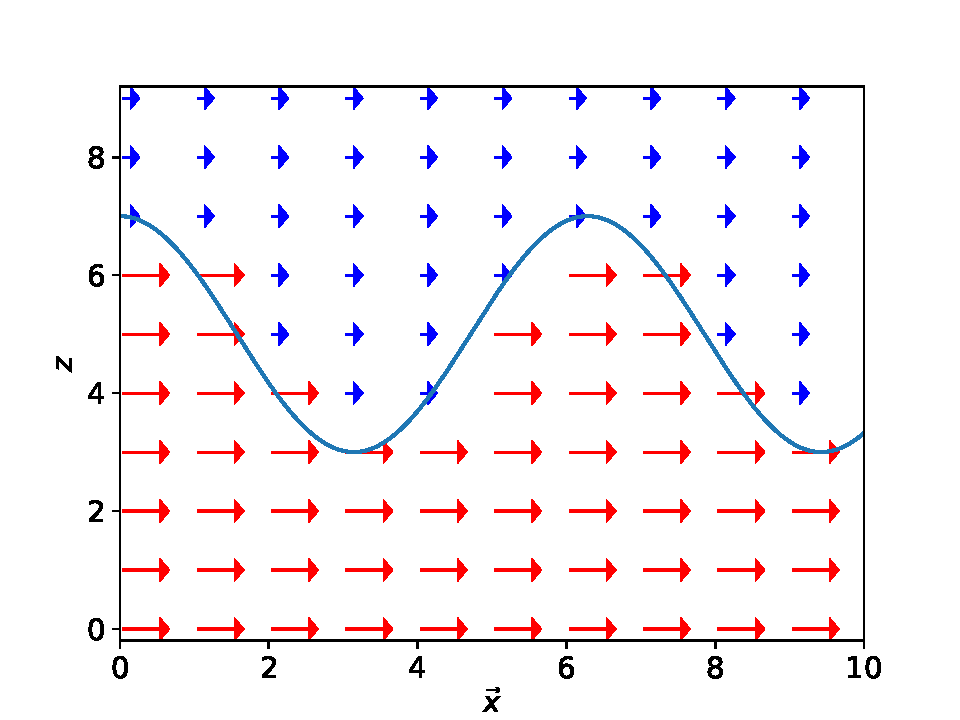
\includegraphics[width=0.5\linewidth]{pop/ab-phi.pdf}
    \caption{Schéma d'un écoulement uniforme parallèle à l'interface dépendant de la phase. Ici, on prend un modèle d'interface \ref{ab-interface} avec $\psi(\vec{x})=\psi_2$ en dessous de linterface et $\phi(\vec{x})=\psi_1$ au dessus. }
\end{figure}

Le second Hamitlonien $H_2$ est pris pour un couplage quadratique entre les deux champs
\begin{equation}
H_2 =\int d\vec{x} \frac{\lambda}{2}(1-\psi(\vec{x})-\phi(\vec{x}))^2,
\end{equation}
où l'on considère la conservation du volume totale des fractions des phases. Le champ $\phi$ peut se comprendre comme la fraction volumique locale d'un solvant d'un système de colloïdes. L'objectif de ce champ est de proposer des particules qui ne sont pas concernées par l'écoulement, peut-être parce qu'elles bougent à une échelle de temps bien plus longue. La présence de ce champ ne change cependant rien aux propriétés à l'équilibre du champ de colloïdes $\psi$. 
L'ajout de ce champ couplé permet de supprimer l'invariance galiléenne par rapport à la vitesse moyenne provoquée par l'écoulement. 

La fonction de partition s'écrit 
\begin{equation}
Z = \int d[\phi]d[\psi]\exp(-\beta H_1[\psi]- \beta H_2[\psi,\phi]) = CZ_{eff},
\end{equation}
{\color{red} expliciter l'étape d'intégration}
où $Z_{eff}$ est une fonction de partition effective ne dépendant que du champ $\psi$.
is the effective partition function for the field $\psi$, after we have integrated out the degrees of freedom corresponding to the field $\phi$,
and $C$ is a constant term resulting from this integration. The effective partition function is thus simply given by

La nouvelle fonction de partition est alors 
\begin{equation}
    Z_{eff} = \int d[\psi]\exp(-\beta H_1[\psi]),
\end{equation}
Comme expliqué plus haut, on voit que le champ $\phi$ n'a plus aucun effet sur les propriétés statistiques à l'équilibre du champ $\psi$.


On considère maintenant la dynamique de schamps. On prend la modèle de diffusivité local (modèle B selon la classification d'Hohenberg et Halpering) pour le champ $\psi$ tandis que l'on prend un modèle non conservé (modèle A) pour le solvant $\phi$.
\begin{align}
    \frac{\partial \psi(\vec{x},t)}{\partial t} +\vec{v}\cdot \vec{ \nabla}\psi(\vec{x},t)&= D\nabla^2\frac{\delta H}{\delta \psi(\vec{x})}+ \sqrt{2D T}\nabla \cdot {\bm \eta}_1(\vec{x},t) \\
    \frac{\partial \phi(\vec{x},t)}{\partial t} &= -\alpha\frac{\delta H}{\delta \phi(\vec{x})}+ \sqrt{2\alpha T}{ \eta}_2(\vec{x},t).
\end{align}
La première équation correspond à une diffusivitié locale $D$ et un terme d'advection par une champ de vitesse contstant $\vec{v}$ . La seconde équation correspond juste à l'équation du modèle A, avec un coefficient cinétique $\alpha$ correspondant au temps de relaxation du système vers l'équilibre. 


The second equation has no advection term and is simple model A dynamics. In principle we can also treat the case where the dynamics of the field $\phi$ is also diffusive and thus of model $B$ type, the analysis given here can be extended to this case but the analysis of the resulting equations is considerably more complicated. The use of model A dynamics for the solvent is justified by assuming that its dynamics is faster than that of the colloids and that the volume fraction can vary due to local conformational changes rather than  diffusive transport.

The noise terms above 
are uncorrelated and Gaussian with zero mean, their correlation functions are given by
\begin{eqnarray}
\langle \eta_{1i}(\vec{x},t) \eta_{1j}(\vec{x}',t)\rangle&=& \delta_{ij}\delta(t-t') \delta(\vec{x}-\vec{x}') \\
\langle \eta_{2}(\vec{x},t) \eta_{2}(\vec{x}',t)\rangle&=& \delta(t-t') \delta(\vec{x}-\vec{x}') ,
\end{eqnarray}
and $T$ is the temperature in units where $k_B=1$.
These dynamical equations  are thus explicitly given by
\begin{equation}
\frac{\partial \psi(\vec{x},t)}{\partial t} +\vec{v}\cdot { \nabla}\psi(\vec{x},t)= D\nabla^2[\frac{\delta H_1}{\delta \psi(\vec{x})}+\lambda(\phi(\vec{x},t) + \psi(\vec{x},t))]+ \sqrt{2D T}\nabla \cdot {\boldsymbol \eta}_1(\vec{x},t)
\end{equation}
and
\begin{equation}
\frac{\partial \phi(\vec{x},t)}{\partial t} = -\alpha\lambda[\phi(\vec{x},t) + \psi(\vec{x},t)]+ \sqrt{2\alpha T}{ \eta}_2(\vec{x},t).
\end{equation}
Taking the temporal Fourier transform, defined with the convention
\begin{equation}
\tilde F(\vec{x}, \omega) = \int_{-\infty}^\infty dt \exp(-i\omega t)F(\vec{x}, t),
\end{equation}
we can eliminate the field $\tilde \phi$ which is given by
\begin{equation}
\tilde \phi(\vec{x},\omega) = \frac{-\alpha\lambda \tilde \psi(\vec{x},\omega)+\sqrt{2\alpha T}\tilde \eta_2(\vec{x},\omega)}{i\omega +\alpha \lambda},
\end{equation}
this then gives the closed equation for $\tilde \psi$:
\begin{equation}
\left[1-\frac{\lambda D \nabla^2}{i\omega+\alpha\lambda}\right]i\omega \tilde\psi(\vec{x}, \omega) +\vec{v}\cdot\nabla\tilde\psi(\vec{x}, \omega)
= D\nabla^2 \tilde \mu(\vec{x},\omega) +  \tilde \zeta(\vec{x},\omega),
\end{equation}
where 
\begin{equation}
\mu(\vec{x},t)=\frac{\delta H_1}{\delta \psi(\vec{x},t)}
\end{equation}
is the effective chemical potential associated with the field $\psi$ and the noise term is given by
\begin{equation}
\tilde \zeta(\vec{x},\omega) = \frac{\sqrt{2\alpha T}D\lambda}{i\omega + \alpha\lambda}\nabla^2\tilde \eta_2(\vec{x},\omega) +
\sqrt{2DT}\nabla\cdot\tilde {\bm \eta}_1(\vec{x},\omega).
\end{equation}
Inverting the temporal Fourier transform then gives the effective evolution equation
\begin{equation}
\frac{\partial \psi(\vec{x},t)}{\partial t} -\lambda D\nabla^2\int_{-\infty}^t dt'
\exp(-\alpha\lambda(t-t')) \frac{\partial \psi(\vec{x},t')}{\partial t}+\vec{v}\cdot\nabla\psi(\vec{x}, t)=D\nabla^2  \mu(\vec{x},t') +  \zeta(\vec{x},t).\label{dyn1}
\end{equation}
\section{Effective interface dynamics}
We now follow the method of \cite{bray2001,bray2002} to derive the dynamical equation  for the interface between the two phases. It is assumed that the driving is in the ${\bf r}=(x,y)$ plane and that the system varies from phase $1$ to phase $2$ in the $z$ direction. The dynamical evolution for the field $\psi$ in Eq. (\ref{dyn1}) is first written as
\begin{equation}
\nabla^{-2}\left[\frac{\partial \psi(\vec{x},t)}{\partial t}+\vec{v}\cdot\nabla\psi(\vec{x}, t)\right] -\lambda D\int_{-\infty}^t dt'
\exp(-\alpha\lambda(t-t')) \frac{\partial \psi(\vec{x},t')}{\partial t'}=D  \mu(\vec{x},t') + \nabla^{-2} \zeta(\vec{x},t).\label{eqpsi}
\end{equation}
We now assume that the field $\psi$ can be written in the form
\begin{equation}
\psi(\vec{x},t) = f(z-h({\bf r},t)),
\end{equation}
and $f(z)\to \psi_2$ as $z\to -\infty$ and $f(z)\to \psi_2$ as  $z\to \infty$.
We now note the following results
\begin{eqnarray}
\frac{\partial f(z-h({\bf r},t))}{\partial t} &=& -f'(z-h({\bf r},t))\frac{h({\bf r},t)}{\partial t}\\
\nabla f(z-h({\bf r},t) )&=& [{\bf e}_z -\nabla h({\bf r},t)]f'(z-h({\bf r},t))]\\
\nabla^2 f(z-h({\bf r},t)) &=& f''(z-h({\bf r},t)[1 + [\nabla h({\bf r},t)]^2] -\nabla^2 h({\bf r},t)f'(z-h({\bf r},t)),
\end{eqnarray}
and thus we find
\begin{equation}
\mu(\vec{x},t)= -\kappa\left(f''(z-h({\bf r},t)[1 + \nabla^2 h({\bf r},t)] -\nabla^2 h({\bf r},t)f'(z-h({\bf r},t))\right) + V'(f(z-h({\bf r},t)) - gz .
\end{equation}
Multiplying both sides of the above by $f'(z-h({\bf r},t))$ yields
\begin{eqnarray}
&&f'(z-h({\bf r},t))\mu(\vec{x},t)=\nonumber \\
 &&-\kappa\left(f'(z-h({\bf r},t)f''(z-h({\bf r},t)[1 + \nabla^2 h({\bf r},t)] -\nabla^2 h({\bf r},t)f'(z-h({\bf r},t))^2\right) + V'(f(z-h({\bf r},t))f'(z-h({\bf r},t))\nonumber \\
 &&- gz f'(z-h({\bf r},t)) \nonumber
\end{eqnarray}
and then integrating over $z$ we obtain
\begin{eqnarray}
\int_{-\infty}^\infty dz f'(z-h({\bf r},t)\mu(\vec{x},t)&=& \kappa \nabla^2 h({\bf r},t)\int_{-\infty}^\infty dz\ f'(z-h({\bf r},t))^2 - \int_{-\infty}^\infty dz gz f'(z-h({\bf r},t))\nonumber \\&=&
\kappa\nabla^2 h({\bf r},t)\int_{-\infty}^\infty dz'\ f'(z')^2 - \int_{-\infty}^\infty dz' g(z' +h({\bf r},t)) f'(z')\nonumber \\
&=& \kappa\nabla^2 h({\bf r},t)\int_{-\infty}^\infty dz' \ f'(z')^2 -\Delta\psi g h({\bf r},t).
\end{eqnarray}
In the above we have assumed that $\int_{-\infty}^\infty dz' z'f'(z')=0$ by symmetry (this is also consistent with the approximation made later on in Eq. (\ref{eqdelta})). Furthermore one can show that \cite{bray2001,bray2002}
\begin{equation}
\kappa\int_{-\infty}^\infty dz' \ f'(z')^2 = \sigma,\label{mfsig}
\end{equation}
where $\sigma$ is the mean-field equilibrium Cahn-Hilliard estimate of the surface tension, obtained by  assuming that $f(z)=\psi_{MF}(z)$ is the equilibrium mean field profile of the field 
$\psi$. We thus find
\begin{equation}
\int_{-\infty}^\infty dz f'(z-h({\bf r},t)\mu(\vec{x},t) = \sigma[\nabla^2 h({\bf r},t)-m^2 h({\bf r},t)]
\end{equation}
where $m^2 = \Delta\psi g /\sigma$. We now carry out the same operation on the left hand side of Eq. (\ref{eqpsi}). First we have
\begin{eqnarray}
\nabla^{-2}\frac{\partial \psi(\vec{x},t)}{\partial t}&+&\vec{v}\cdot\nabla \psi(\vec{x},t) +\lambda D\int_{-\infty}^t dt'
\exp(-\alpha\lambda(t-t')) \frac{\partial \psi(\vec{x},t')}{\partial t'} = \nonumber \\ 
&-&\nabla^{-2}f'(z-h({\bf r},t))[\frac{\partial h({\bf r},t)}{\partial t} +\vec{v}\cdot\nabla h({\bf r},t)]  +\lambda D\int_{-\infty}^t dt'
\exp(-\alpha\lambda(t-t')) f'(z-h({\bf r},t'))\frac{\partial h({\bf r},t')}{\partial t'}\nonumber \\
&\approx& -\nabla^{-2}f'(z) [\frac{\partial h({\bf r},t)}{\partial t} +\vec{v}\cdot\nabla h({\bf r},t)] +\lambda D\int_{-\infty}^t dt'
\exp(-\alpha\lambda(t-t')) f'(z)\frac{\partial h({\bf r},t')}{\partial t'},\end{eqnarray}
where in the last line above we have neglected terms quadratic in $h$. 
Note that the neglecting of these additional terms is not strictly justified, they could potentially induce non-perturbative effects which render the surface fluctuations non-Gaussian. However we see here that the first order computation we carry out tends to reduce fluctuations with respect to equilibrium or non-driven interfaces and so if the equilibrium theory can be described by an equation which is linear in height fluctuations, it seems physically reasonable to assume that the the approximation also holds for the driven interface. 
Again, we multiply the above by $f'(z)$ and integrate over $z$. In the first term we make use of the approximation
\begin{equation}
f'(z)=\Delta\psi \delta(z)\label{eqdelta}
\end{equation}
and in the second we use the relation in Eq. (\ref{mfsig}). Putting this all together we obtain
\begin{equation}
\Delta\psi^2 \int d{\bf r} G(0,{\bf r}-{\bf r}') [\frac{\partial h({\bf r},t)}{\partial t} +\vec{v}\cdot\nabla h({\bf r},t)] +\frac{\sigma\lambda D}{\kappa}\int_{-\infty}^t dt'
\exp(-\alpha\lambda(t-t'))\frac{\partial h({\bf r},t')}{\partial t'}
= \sigma[\nabla^2 h({\bf r},t)-m^2 h({\bf r},t)] + \xi({\bf r},t),\label{em}
\end{equation}
where $G= -\nabla^{-2}$, or more explicitly
\begin{equation}
\nabla^2 G(z-z',{\bf r}-{\bf r}') = -\delta(z-z') \delta({\bf r}-{\bf r'}).
\end{equation}
The noise term $\xi$ is given by
\begin{equation}
\xi({\bf r},t) = \int_{-\infty}^{\infty} dz f'(z-h({\bf r},t)) \nabla^{-2} \zeta(\vec{x},t).
\end{equation}
Now, as the equations of motion have been derived to first order in $h$ and we wish to recover the correct equilibrium statistics for the non-driven system, we ignore the $h$ dependence in the noise and make the approximation
\begin{equation}
\xi({\bf r},t) \approx \int_{-\infty}^{\infty} dz f'(z) \nabla^{-2} \zeta(\vec{x},t).
\end{equation}
The correlation function of this noise is most easily evaluated in terms of its Fourier transform with respect to  space and time  defined by
\begin{equation}
\hat F({\bf q},\omega)=\int dt d{\bf r}\exp(-i\omega t -i{\bf q}\cdot{\bf r}) F({\bf r},t).
\end{equation}
Using the relations Eqs. (\ref{mfsig}) and (\ref{eqdelta}) one  can show that
\begin{equation}
\langle \hat \xi({\bf q},\omega)\hat \xi({\bf q}',\omega')\rangle 
=2T(2\pi)^d \delta(\omega +\omega') \delta({\bf q}+{\bf q}') \left[
\frac{\sigma}{\kappa}\frac{\alpha D^2\lambda^2}{\omega^2 +\alpha^2\lambda^2} + \frac{D\Delta\psi^2}{2q}\right].
\end{equation}
In full Fourier space the equation of motion for the field $\psi$ then reads
\begin{equation}
\left[i(\omega+{\bf q}\cdot\vec{v})\frac{\Delta\psi^2}{2q} + \frac{D\sigma\lambda}{\kappa} \frac{i\omega}{\alpha\lambda+i\omega}\right] \hat h({\bf q},\omega)= -D\sigma(q^2+m^2)\hat h({\bf q},\omega)+ \hat\xi({\bf q},\omega).\label{dyn}
\end{equation}

From this, the full Fourier transform of the correlation function of the interface height is given by
\begin{equation}
\hat C({\bf q},\omega)  = 2TD \frac{\left[ \frac{\Delta\psi^2}{2q}(\omega^2+\alpha^2 \lambda^2) + \frac{\sigma\alpha D\lambda^2}{\kappa}\right]}{\left|i[\frac{\alpha\lambda\Delta\psi^2}{2 q}(\omega + {\bf q}\cdot\vec{v}) + \frac{\lambda \sigma D}{\kappa}\omega + D\sigma(q^2+m^2)\omega]
+[\alpha\lambda D\sigma(q^2+m^2) -\frac{\Delta\psi^2}{2q}\omega(\omega+{\bf q}\cdot\vec{v})]\right|^2}.
\end{equation}
Using the above we can extract the equal time height-height correlation function in the steady states. Its spatial Fourier transform can shown to be given by
\begin{eqnarray}
\tilde C_s({\bf q}) &=& \frac{1}{2\pi} \int d\omega \hat C({\bf q}, \omega)\nonumber\\
&=&T \frac{\left(2 D\sigma q(\kappa[q^2+m^2]+\lambda)+\alpha\kappa\lambda\Delta\psi^2\right)^2 +\kappa^2 \Delta\psi^4 ({\bf q}\cdot\vec{v})^2}{\sigma[q^2+m^2]\left(2D q\sigma (\kappa[q^2+m^2]+\lambda)+\alpha \kappa\lambda \Delta\psi^2\right)^2 + \kappa\left(\kappa\sigma[q^2+m^2] + \lambda\sigma\right)\Delta\psi^4({\bf q}\cdot\vec{v})^2}.\label{eqmaind}
\end{eqnarray}
An outline of the derivation of this result is given in the Appendix to the paper.
In the absence of driving, {\em i.e.} when $\vec{v}={\bf 0}$ we recover the equilibrium correlation function
\begin{equation}
\tilde C_s({\bf q})= \tilde C_{eq}({\bf q})= \frac{T}{\sigma[q^2+m^2]},
\end{equation} 
here we see that  $1/m= \xi_{eq}$ is the so called capillary length, which is the equilibrium correlation length of the height fluctuations. We also notice that the correlation function for wave vectors perpendicular to the driving direction is simply the equilibrium one.

If we write $C_s({\bf q})= T/H_s({\bf q})$ we can interpret $H_s({\bf q})$ as an effective quadratic Hamiltonian for the height fluctuations, it is thus given by
\begin{equation}
H_s({\bf q}) = \sigma[q^2+m^2] + \frac{\kappa\lambda\sigma \Delta\psi^4 ({\bf q}\cdot\vec{v})^2}{\left(2 D\sigma q(\kappa[q^2+m^2]+\lambda)+\alpha\kappa\lambda\Delta\psi^2\right)^2 +\kappa^2 \Delta\psi^4 ({\bf q}\cdot\vec{v})^2}
\end{equation}
For small $q$ we find 
\begin{equation}
H_s({\bf q}) = \sigma m^2 + \sigma q^2(1+ \frac{v^2\cos^2(\theta)}{\alpha^2\lambda\kappa}),
\end{equation}
where $\theta$ is the angle between the wave vector ${\bf q}$ and the direction of the driving. 
This thus gives a direction dependent surface tension 
\begin{equation}
\sigma_s(\theta) = \sigma(1+ \frac{v^2\cos^2(\theta)}{v^2_0}),
\end{equation}
where we have introduced the intrinsic velocity $v_0 = \sqrt{\alpha^2\lambda\kappa}$ which depends on the microscopic {\em dynamical} quantity $\alpha$ associated with the model A dynamics of the field $\phi$, as well as the microscopic static quantities $\kappa$ (which generates the surface tension) and $\lambda$ the coupling between the field $\psi$ and $\phi$. This appearance of dynamical and static quantities that are otherwise hidden in equal time correlation functions in equilibrium is already implicit in the works of Onsager \cite{hem1996} where it is used to compute the conductivity of Brownian electrolytes and the explicit expressions were derived using stochastic density functional theory in \cite{dem2016}. We also note that the universal thermal Casimir effect between model Brownian electrolyte systems  driven by an electric field 
exhibits similar features, developing a dependency on both additional static and dynamical variables with respect to the equilibrium case \cite{dean2016}


However for this small $q$ expansion we see that the microscopic 
quantities $D$, the diffusion constant of the field $\phi$, and the order parameter jump
$\Delta\psi$ do not appear. 

From the above, we see that  in the direction of the driving the surface tension increases and the fluctuations of the surface are thus suppressed. We may also write 
\begin{equation}
H_s({\bf q}) = \sigma_s(\theta) [q^2 + m^2_e(\theta)],
\end{equation}
with 
\begin{equation}
m^2_s(\theta) =\frac{ m^2}{1+ \frac{v^2\cos^2(\theta)}{v_0^2}},
\end{equation}
this corresponds to a correlation length 
\begin{equation}
\xi_s = \xi_{eq}\sqrt{1+ \frac{v^2\cos^2(\theta)}{v_0^2}},
\end{equation}
and we see that it is increased in the direction of the driving. 

As we have just remarked  that the above results appear to be independent of the order parameter jump $\Delta \psi$ and the diffusion constant $D$, however the next order correction to $H_s$ for small $q$ is given by
\begin{equation}
H_s({\bf q}) = \sigma_s(\theta) [q^2 + m^2_e(\theta)] - \frac{4Dq \sigma^2(\lambda+\kappa m^2)( {\bf q}\cdot\vec{v})^2 }{\alpha^3 \kappa^2 \lambda^2 \Delta\psi^2},
\end{equation}
and so the small ${\bf q}$ expansion  breaks down at $\Delta\psi=0$, indeed one can see that the system has exactly the equilibrium correlation function when  $\Delta\psi=0$. 

In the limit of large $q$ we see that the effective Hamiltonian is given, to leading order, by the original equilibrium Hamiltonian and so the out of equilibrium driving has no effect on the most energetic modes of the system.

The results here predict that for unconfined surfaces the long range height fluctuations are described by an isotropic form of capillary wave theory with 
an anisotropic surface tension which is largest in the direction of driving. Numerical simulations of driven lattice gases in two dimensions \cite{leun1993} show a more drastic change upon driving and find $C_s(q)\sim  1/q^{.66}$ and thus a strong deviation from capillary wave theory.  
\section{A model of active interfaces}
We can apply the results derived in the previous section to analyse a simple model for
surfaces formed between two phases of active colloids. Activity is modelled by assuming that the colloidal field $\psi$ has a temperature different to that of  the solvent field $\phi$. This models the effect that activity leads to enhanced colloidal diffusivity over and
above the Brownian motion of particles due to thermal fluctuations \cite{gros2015}.

In the absence of any driving the dynamical equations for the field $\psi$ and $\phi$ become 
\begin{eqnarray}
\frac{\partial \psi(\vec{x},t)}{\partial t} &=& D\nabla^2\frac{\delta H}{\delta \psi(\vec{x})}+ \sqrt{2D T_1}\nabla \cdot {\bm \eta}_1(\vec{x},t) \\
\frac{\partial \phi(\vec{x},t)}{\partial t} &=& -\alpha\frac{\delta H}{\delta \phi(\vec{x})}+ \sqrt{2\alpha T_2}{ \eta}_2(\vec{x},t).
\end{eqnarray}
Following the same arguments as above we find that
\begin{equation}
\hat C({\bf q},\omega)  = 2D \frac{\left[ T_1\frac{\Delta\psi^2}{2q}(\omega^2+\alpha^2 \lambda^2) + T_2\frac{\sigma\alpha D\lambda^2}{\kappa}\right]}{\left|i\omega[\frac{\alpha\lambda\Delta\psi^2}{2 q} +  \frac{\lambda \sigma D}{\kappa} + D\sigma(q^2+m^2)]
+[\alpha\lambda D\sigma(q^2+m^2) -\frac{\Delta\psi^2}{2q}\omega^2]\right|^2}.
\end{equation}
The equal time steady state height fluctuations thus have correlation function
\begin{equation}
\tilde C_s(q) = \frac{T_1}{\sigma (q^2 + m^2)}\left[ 1 -(1-\frac{T_2}{T_1})\frac{\lambda\sigma } {\kappa }\frac{1}{\frac{\alpha\lambda \Delta \psi^2}{2Dq}+ \frac{\lambda\sigma }{\kappa} + \sigma(q^2+m^2)}\right].
\end{equation}
We see, again, that the inclusion of a non-equilibrium driving changes the statistics of height fluctuations and leads to a steady state that depends on both dynamical variables
$D$ and $\alpha$ as well as static ones $\Delta\psi,\ \lambda$ and $\kappa$ that remain hidden in the equilibrium case. This phenomenon is again seen in the behavior of the universal thermal  Casimir force between Brownian conductors held at different temperatures \cite{lu2015}.

If we assume strong activity we can take the limit $T_1\gg T_2$, in this case we find
\begin{equation}
\tilde C_s(q) = \frac{T_1}{\sigma (q^2 + m^2)}\frac{\frac{\alpha\lambda \Delta \psi^2}{2Dq}+
\sigma(q^2+m^2)}{\frac{\alpha\lambda \Delta \psi^2}{2Dq}+ \frac{\lambda\sigma }{\kappa} + \sigma(q^2+m^2)}.
\end{equation}
Interpreted in terms of an effective Hamiltonian for an equilibrium system at the temperature $T_1$ the above gives
\begin{equation}
H_s(q) = \sigma (q^2 + m^2)\left[1+\frac{\lambda\sigma }{\kappa}\frac{q}{\frac{\alpha\lambda \Delta \psi^2}{2D}+
q\sigma(q^2+m^2)}\right].
\end{equation}
In the case of an unconfined interface (where there is no gravitational effect
on the surface fluctuations) {\em i.e.} $m=0$ we see that for small $q$
\begin{equation}
H_s(q) \approx \sigma q^2 +\frac{2D\sigma^2 }{\kappa\alpha \Delta\psi^2}q^3 .
\end{equation}
We see that the effective surface tension is not modified but a reduction of fluctuations due to the presence of the term in $q^3$ arises.  As in the case of a driven system, we see that the large $q$ behavior of the effective Hamiltonian is given by the equilibrium case where $T=T_1=T_2$. 

In the case where the interface is confined, we see that for small $q$ one obtains
\begin{equation}
H_s(q) \approx \sigma m^2 \left[ 1+ \frac{2D\sigma }{\kappa\alpha \Delta\psi^2}q\right],
\end{equation}
and thus at the largest length scales of the problem there is a qualitative departure from capillary wave behavior, and the correlation length of height fluctuations at the largest length scales is given by
\begin{equation}
\xi_s = \frac{2D\sigma }{\kappa\alpha \Delta\psi^2}.
\end{equation}
The above result should be compared with that obtained in \cite{zia1991} for 
systems with anisotropic thermal white noise, which breaks detailed balance and mimics random driving of the system parallel to the interface; for free interfaces it was found that $C_s(q)\sim 1/q$.
\section{Conclusions}
We have presented a model to analyse the effect of uniform driving on the dynamics of the interface in a two phase system. In order to generate a non-equilibrium state a second {\em hidden} order parameter was introduced. This models the behaviour of a local or solvent degree of freedom which is not influenced by the driving field. In this way, we obtain out of equilibrium interface fluctuations which are described by Gaussian statistics as found in the experimental study of \cite{derks2006}. The agreement with this experimental study also extends to qualitative agreement with the increase of the effective surface tension in the direction of driving and also an increase in the correlation length of the height fluctuations with respect to a non-driven equilibrium interface. However, we  note that numerical simulations of a sheared Ising interface \cite{smith2008,smith2010} also reveal a reduction of interface fluctuations but the lateral correlation length is found to be reduced.

The basic idea underlying this study would be interesting to apply to a number of possible variants of this model, for instance both the dynamics
of the main field $\phi$ and the solvent field $\phi$ could be varied. To make a direct link with driven colloidal interfaces one should study model H type dynamics for the main field $\phi$ and other variants for the dynamics of the 
solvent field $\phi$ could also be considered. 

As mentioned above, in lattice based models driving induces non-equilibrium states even in the simple Ising lattice gas. A model analogous to that studied here can be formulated in a lattice based systems using the Hamiltonian 
\begin{equation}
H = -J\sum_{(ij)}S_i S_j (1+ \sigma_{(ij)}),
\end{equation}
where $S_i=\pm1$ are Ising spins at the lattice sites $i$, and $\sigma_{(ij)}=\pm 1$ are Ising like dynamical solvent variables associated with the lattice links $(ij)$. The static partition function is given by
\begin{equation}
Z = {\rm Tr}_{\sigma_{ij},S_i} \exp\left[\beta J\sum_{(ij)}S_i S_j (1+ \sigma_{(ij)})\right],
\end{equation}
and the trace over the solvent variables can be trivially carried out to give
\begin{equation}
Z = {\rm Tr}_{S_i}\left( \exp\left[\beta J\sum_{(ij)}S_i S_j \right]\prod_{(ij)}2\cosh(\beta JS_iS_j)\right )= [2\cosh(\beta J)]^L{\rm Tr}_{S_i}\exp(\beta J\sum_{(ij)}S_i S_j ),
\end{equation}
where $L$ is the number of links on the lattice of the model. We thus see that the underlying effective static model is precisely the zero field Ising model. 

This model can then be driven in a number of ways, for instance using conserved Kawasaki dynamics for the Ising spins to model diffusive dynamics in the presence of a uniform driving field parallel to the surface between the two phases at a temperature below the ferromagnetic ordering temperature $T_c$. The dynamics of the Ising spins on the lattice links can  be given by non-conservative single spin flip, for instance Glauber, dynamics to keep the analogy with the continuum model discussed in the paper but diffusive dynamics or indeed a mixture of diffusive and non-conserved dynamics 
could be implemented. It would be interesting to see to what extent this modification of the driven lattice gas model affects the non-equilibrium driven states that arise. 

It is also clear that this lattice model can be used to simulate the effect of activity where the Ising spins $S_1$ corresponding to the colloid field undergo  Kawasaki dynamics at the temperature $T_1$ where as the link variables $\sigma_{(ij)}$ undergo single spin flip non-conserved dynamics
at the temperature $T_2$.

\section{Acknowledgements}
The authors acknowledge support from the ANR (France) Grant FISICS \\
\appendix
\section{Evaluating Fourier integrals}
Here we outline how the Fourier integration leading to Eq. (\ref{eqmaind}) is carried out. Defining
\begin{equation}
I(f(\omega)) = \int \frac{d\omega}{2\pi} \frac{f(\omega)}{\left|i(A\omega + B) + (C-D\omega-E \omega^2)\right|}
\end{equation}
we see that the integral we need to evaluate can be written in the form
\begin{equation}
I = a I(\omega^2) + b I(1).
\end{equation}
The calculation leading to Eq. (\ref{dyn}) can be carried out in the presence of a forcing term on the height profile in order to compute the response function for the surface which has a denominator of the form
\begin{equation}
{\rm Den} = i(A\omega + B) + (C-D\omega-E \omega^2),
\end{equation}
and due to causality the above only has poles in the upper complex plane (due to the convention of Fourier transforms used here). Consequently we find that
\begin{equation}
\int \frac{d\omega}{2\pi} \frac{1}{i(A\omega + B) + (C-D\omega-E \omega^2)} = 0,\label{key}
\end{equation}
as one may close the integration contour in the lower half of the complex plane. Taking the real and imaginary part of Eq. (\ref{key}) leads to
\begin{eqnarray}
C I(1) -D I(\omega) - E I(\omega^2) = 0 \\
AI(\omega) + B I(1) = 0.
\end{eqnarray}
Using this we can express $I(\omega^2)$ as a function of $I(1)$, and explicitly we have 
\begin{equation}
I(\omega^2) = \frac{I(1)}{E}[C+ \frac{DB}{A}].
\end{equation}

To evaluate $I(1)$ we now use
\begin{equation}
I(1) = -{\rm Im} \int \frac{d\omega}{2\pi}\frac{1}{A\omega +B} \frac{1}{i(A\omega + B) + (C-D\omega-E \omega^2)}.
\end{equation}
The integrand above has no poles in the lower half of the complex plane but has a {\em half pole} at $\omega=-B/A$ on the real axis, thus using standard complex analysis we find
\begin{equation}
I(1) = \frac{1}{2(CA + BD - \frac{EB^2}{A})}.
\end{equation}
Then after some laborious, but straightforward algebra, the results Eq. (\ref{eqmaind}) is obtained.




The dynamics of discrete particle systems is however affected by uniform driving of identical particles. The study of driven lattice gases has revealed a wide range of intriguing physical phenomena and indeed shown how driving can even lead to phase separation \cite{katz1984,zia1991,leun1993,schm1995,schm1998}. The discrete nature of the dynamics of these systems, both in space and time, means that no Galilean transformation to an equilibrium state exists. Analytical studies of these systems require a phase ordering kinetics description in terms of a continuum order parameter. In order to break Galilean invariance the local mobility of the particles can be taken to be dependent on the local order parameter, this is then sufficient to induce non-trivial steady states under driving \cite{katz1984,leun1993,schm1995,schm1998}. Interfaces between the separated phases in uniformly driven systems have non capillary behaviors which are, even today, not fully understood \cite{leun1993}.
Taking random driving in a given direction also leads to non-equilibrium steady states, if the noise is Gaussian and white, the fluctuation dissipation theorem is violated and novel interface fluctuations are induced which, again, are  not of  the capillary type \cite{zia1991}. 



\chapter*{Conclusion et perspectives}
\addcontentsline{toc}{chapter}{Conclusion et perspectives}


\bibliography{biblio.bib}
\end{document}